\documentclass[11pt]{article}
\usepackage{fullpage}
\usepackage{setspace}
\usepackage{amsmath}
\usepackage{fancyvrb}
\usepackage{enumerate}
\usepackage{listings}
\usepackage{pgfplots}
\usepackage{graphicx}
\usepackage{float}
\usepackage{multirow}
\usepackage[format=hang,labelsep=quad]{caption}
\usepackage{subfig}
\usepackage{array}
\usepackage{multirow}

\renewcommand\thesubfigure{\roman{subfigure}}


\begin{document}
\noindent\large{Math 5364}\\
\large{Data Mining 2}\\
\large{Homework 21}\\
\large{Mary Barker}
\doublespace

\begin{enumerate}
\item Remove all categorical variables from the Auto MPG data set from the 
UCI Machine learning Repository, and then examine this data set for anomalies, 
using the following methods for computing outlier scores: 

\begin{itemize}
\item Distance for k-nearest neighbor, where k = 5

\item Density

\item Local Outlier Factor method.
\end{itemize}
 For each of these methods, plot the density of the outlier score, and 
produce scatterplots with a heat map of the outlier scores.  

 Do you have any comments on this data set after performing the outlier analysis? 


\begin{itemize}
\item Using distance, there were two likely looking places for determining 
cutoff for clusters as can be seen from the plot below. The first was at 1.5, and 
the second at 1.25.

\begin{center}
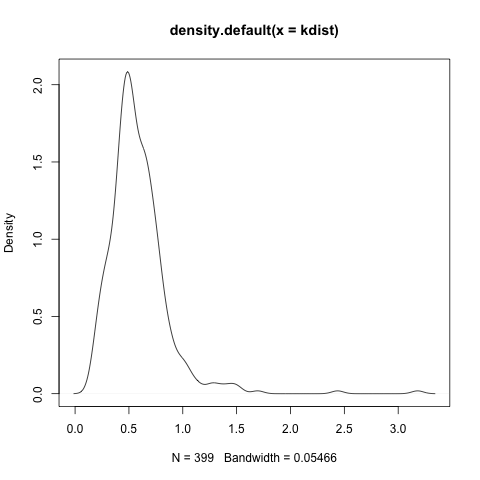
\includegraphics[scale=0.35]{density_kdist}
\end{center}

%    # knn: 
%    kdist = my.kdist(deleted_auto[,cols],5)
%    plot(density(kdist))
%	(1:nrow(deleted_auto))[kdist> 1.5]
%   1  30 113 389
%	(1:nrow(deleted_auto))[kdist>= 1.25]
%   1  30  73 113 211 245 329 335 336 359 366 389

The plot of values for each point using distance as a metric is shown below. 

\begin{figure}[H]
\begin{center}
\subfloat[]{\begin{centering}
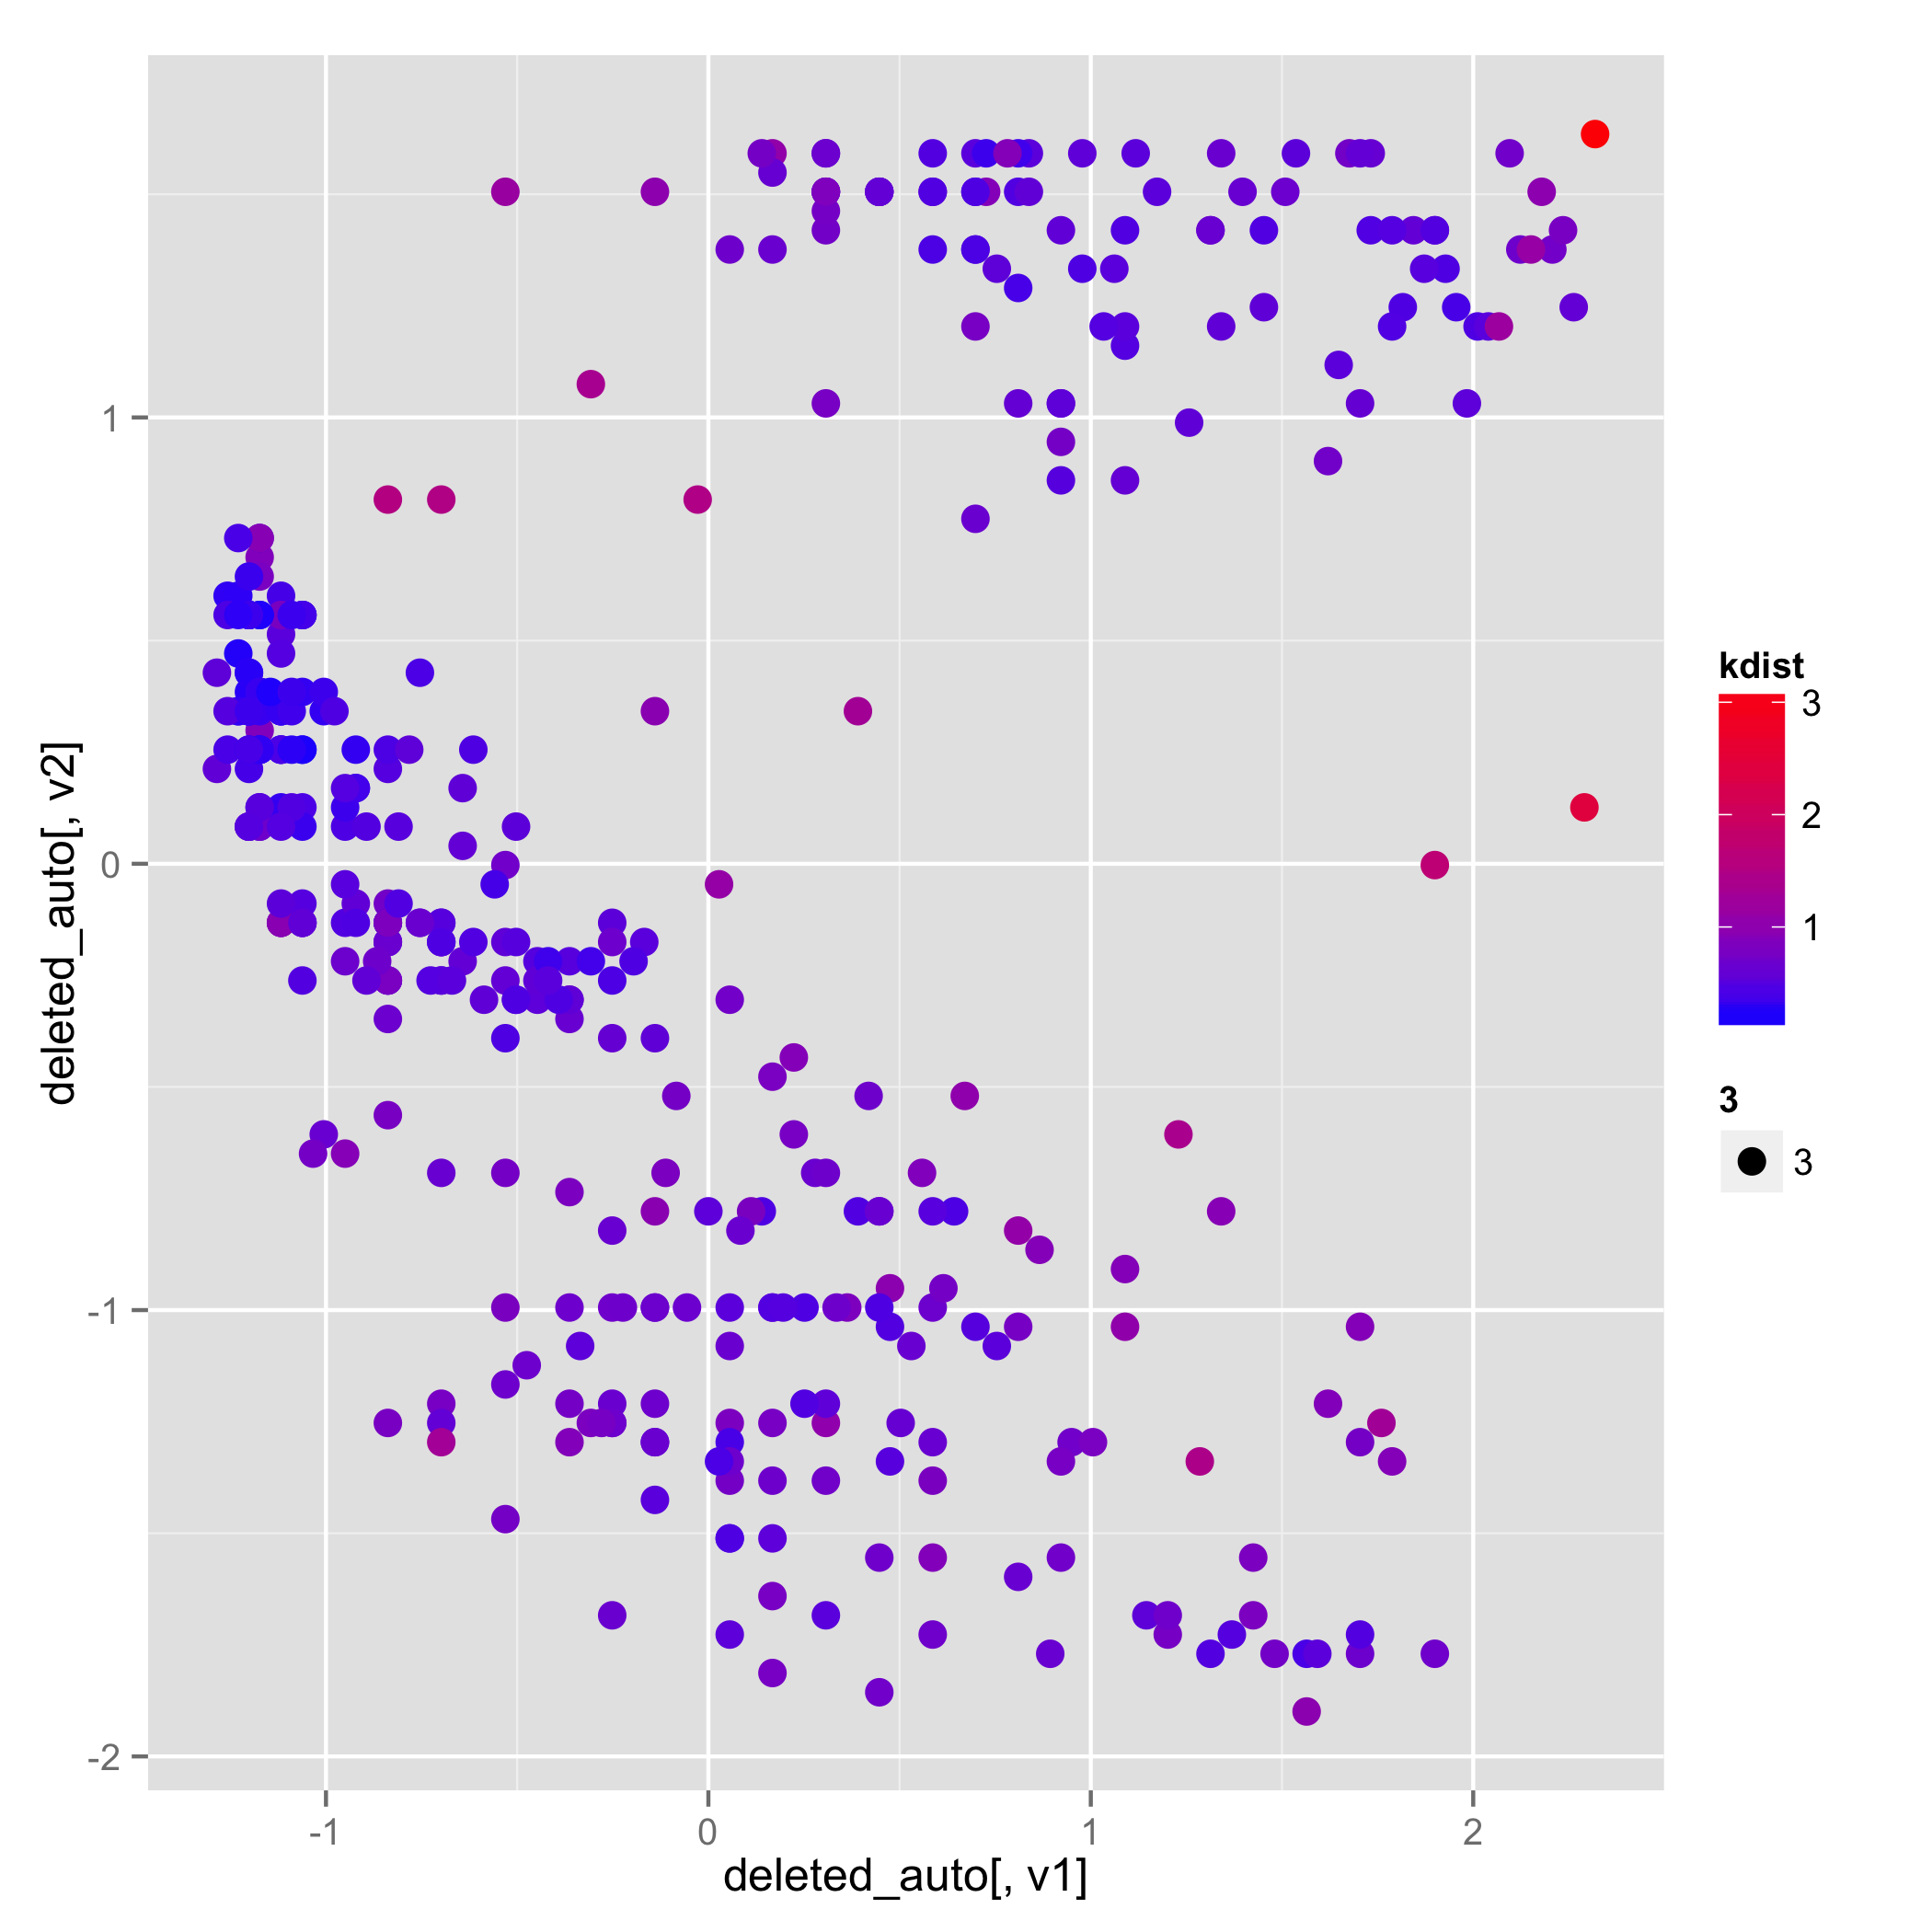
\includegraphics[scale=0.05]{using_kdist1_3.png}
\par\end{centering}}
\quad{}
\subfloat[]{\begin{centering}
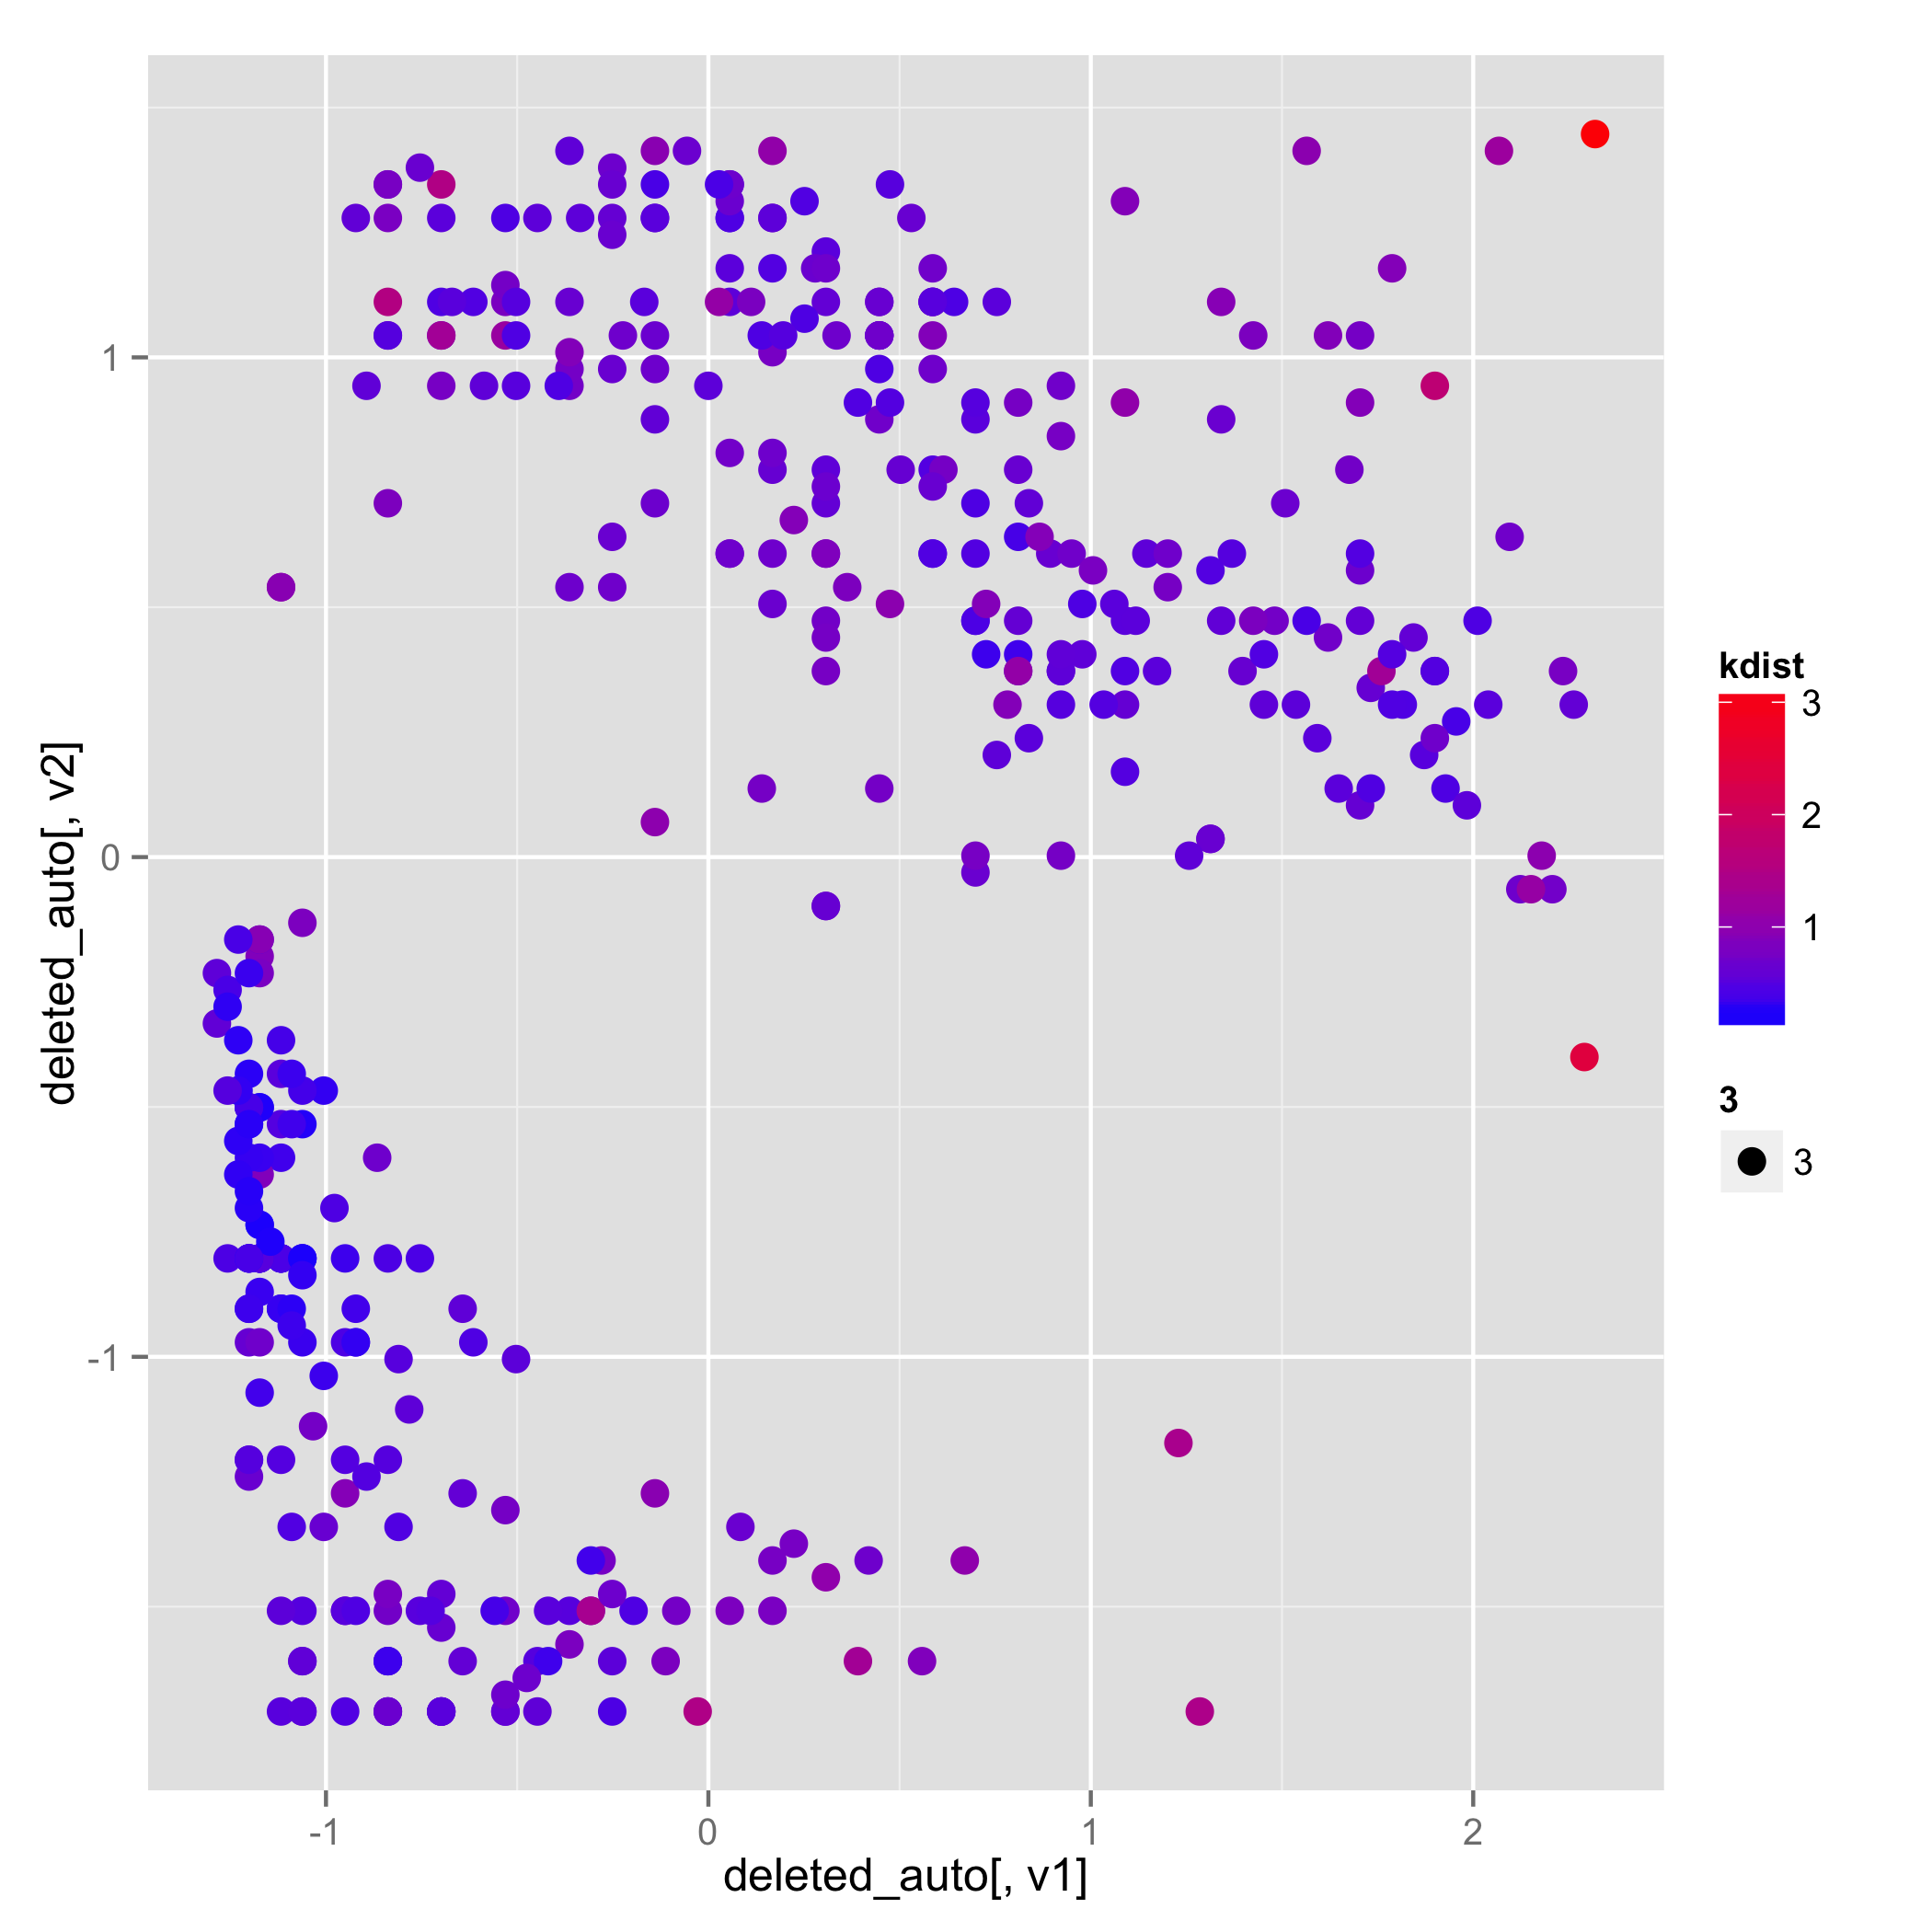
\includegraphics[scale=0.05]{using_kdist1_4.png}
\par\end{centering}}
\quad{}
\subfloat[]{\begin{centering}
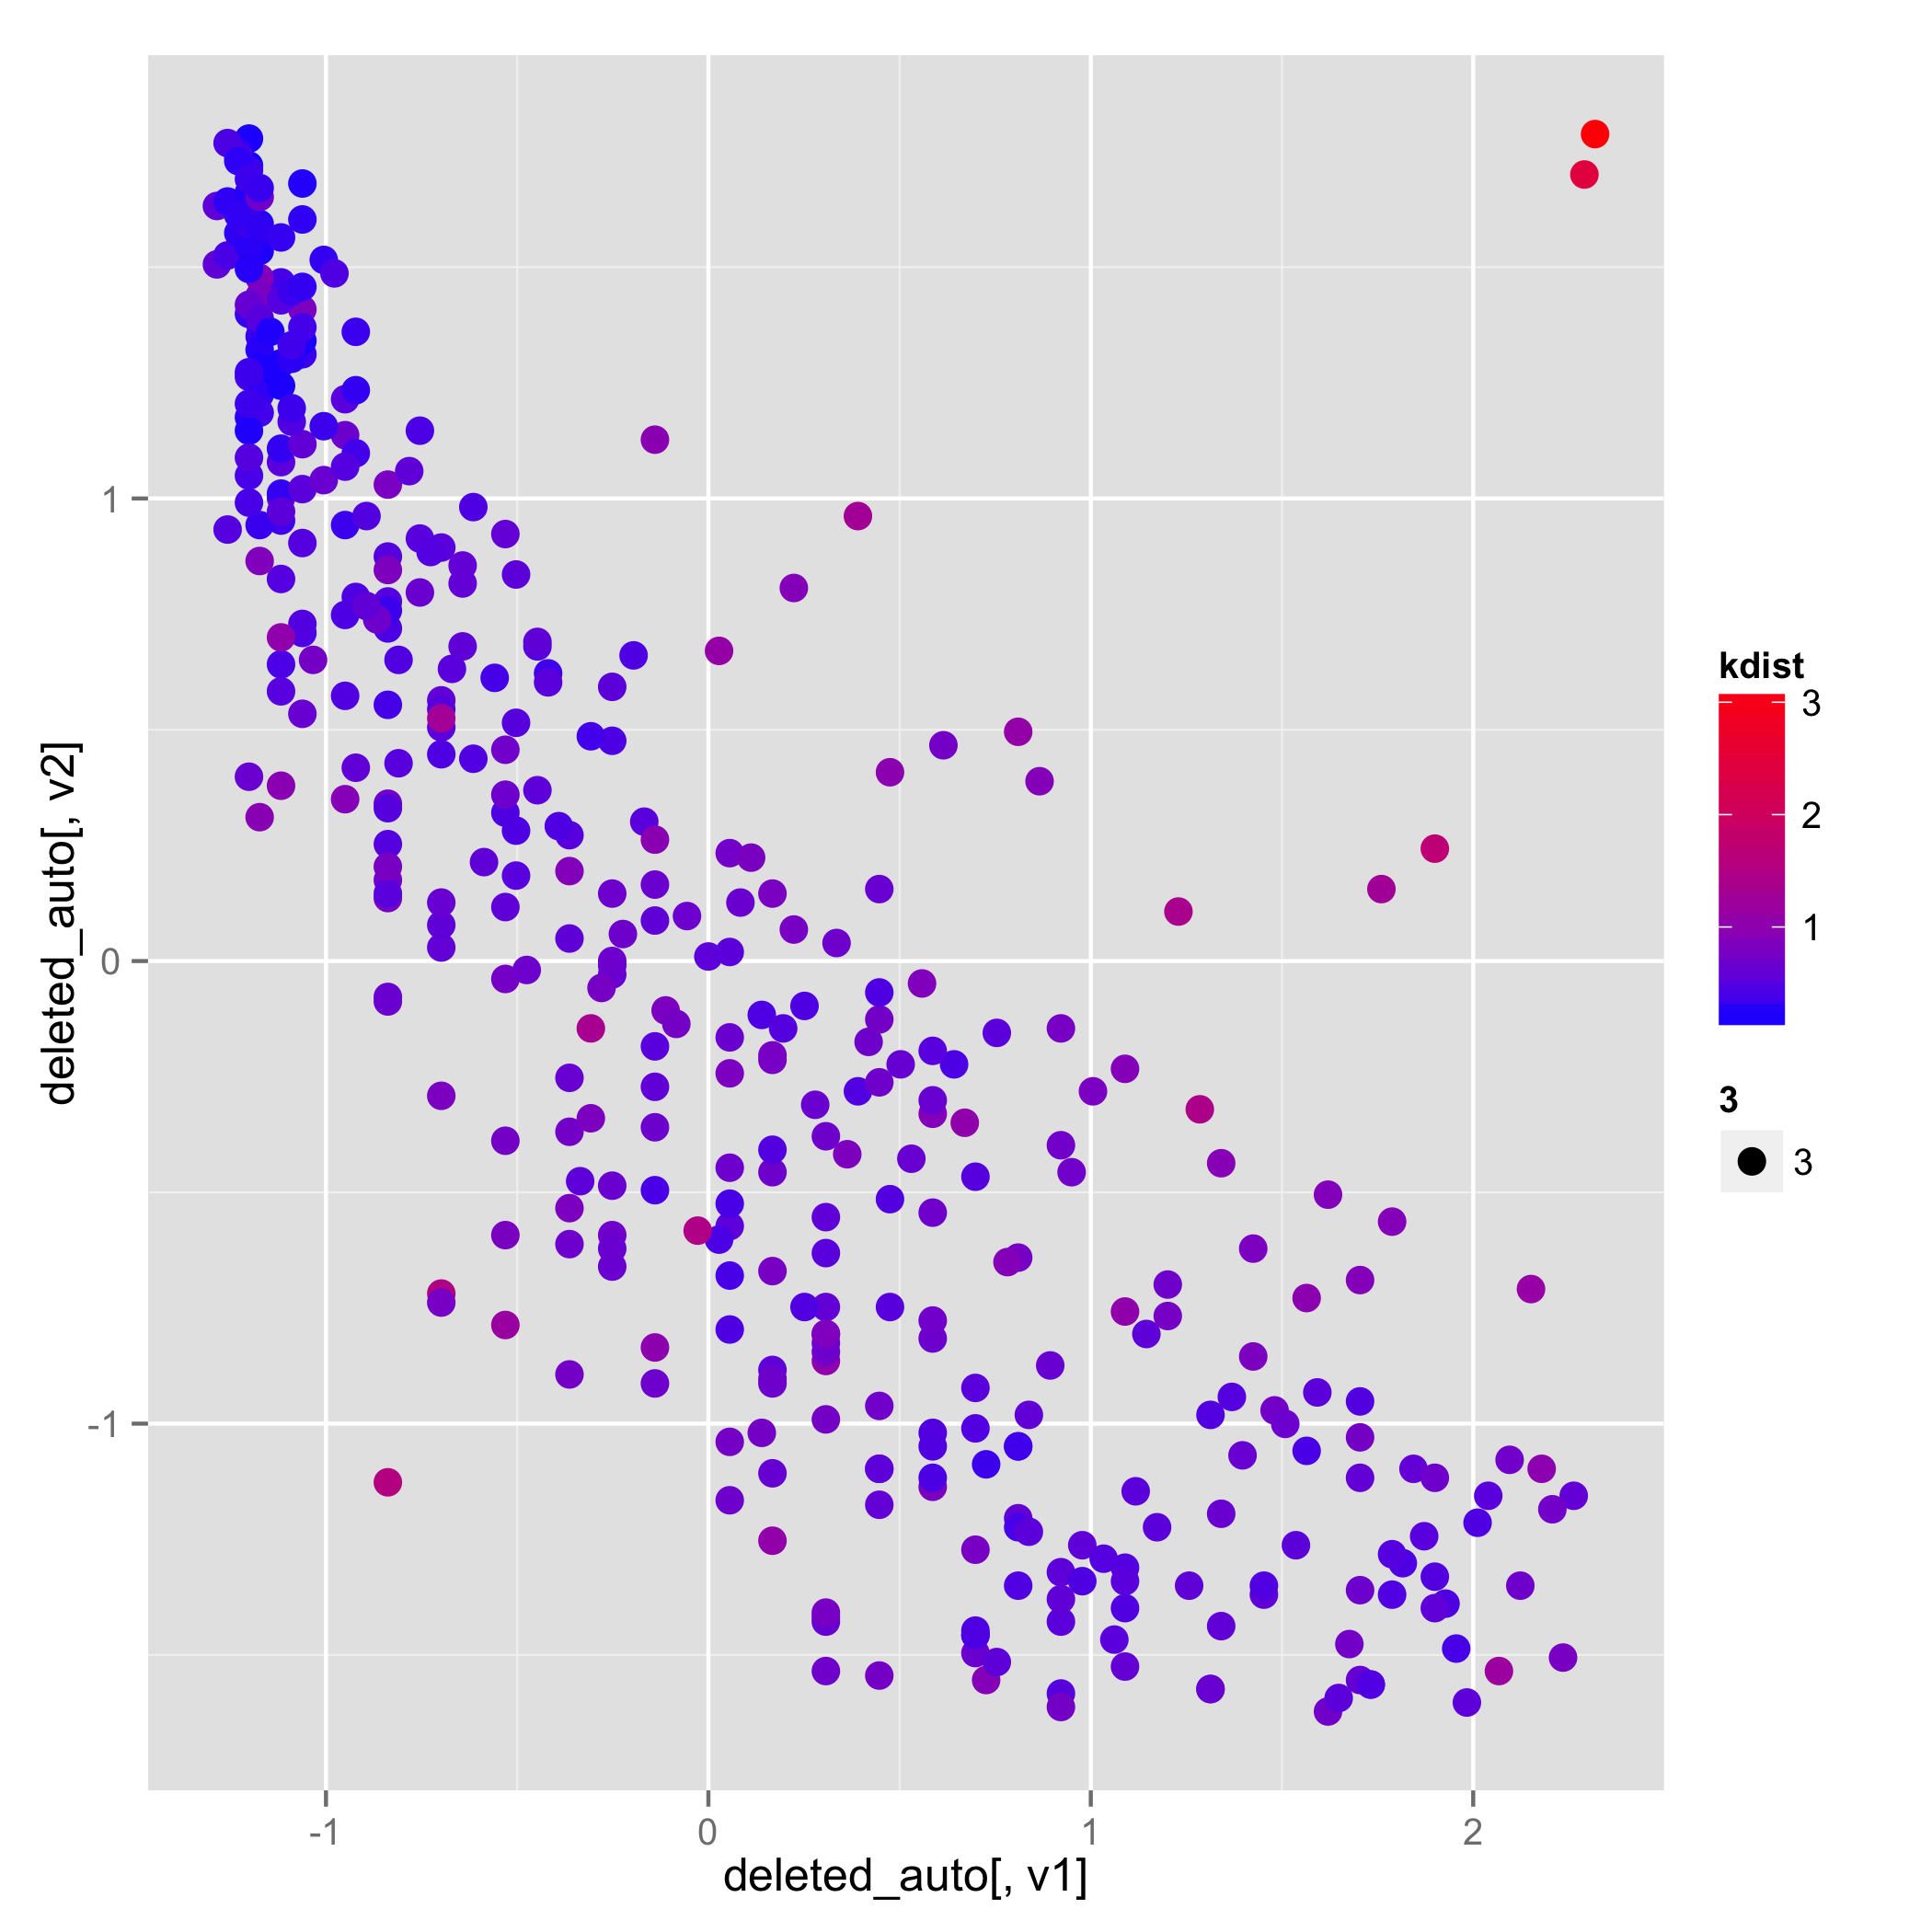
\includegraphics[scale=0.05]{using_kdist1_5.png}
\par\end{centering}}
\quad{}
\subfloat[]{\begin{centering}
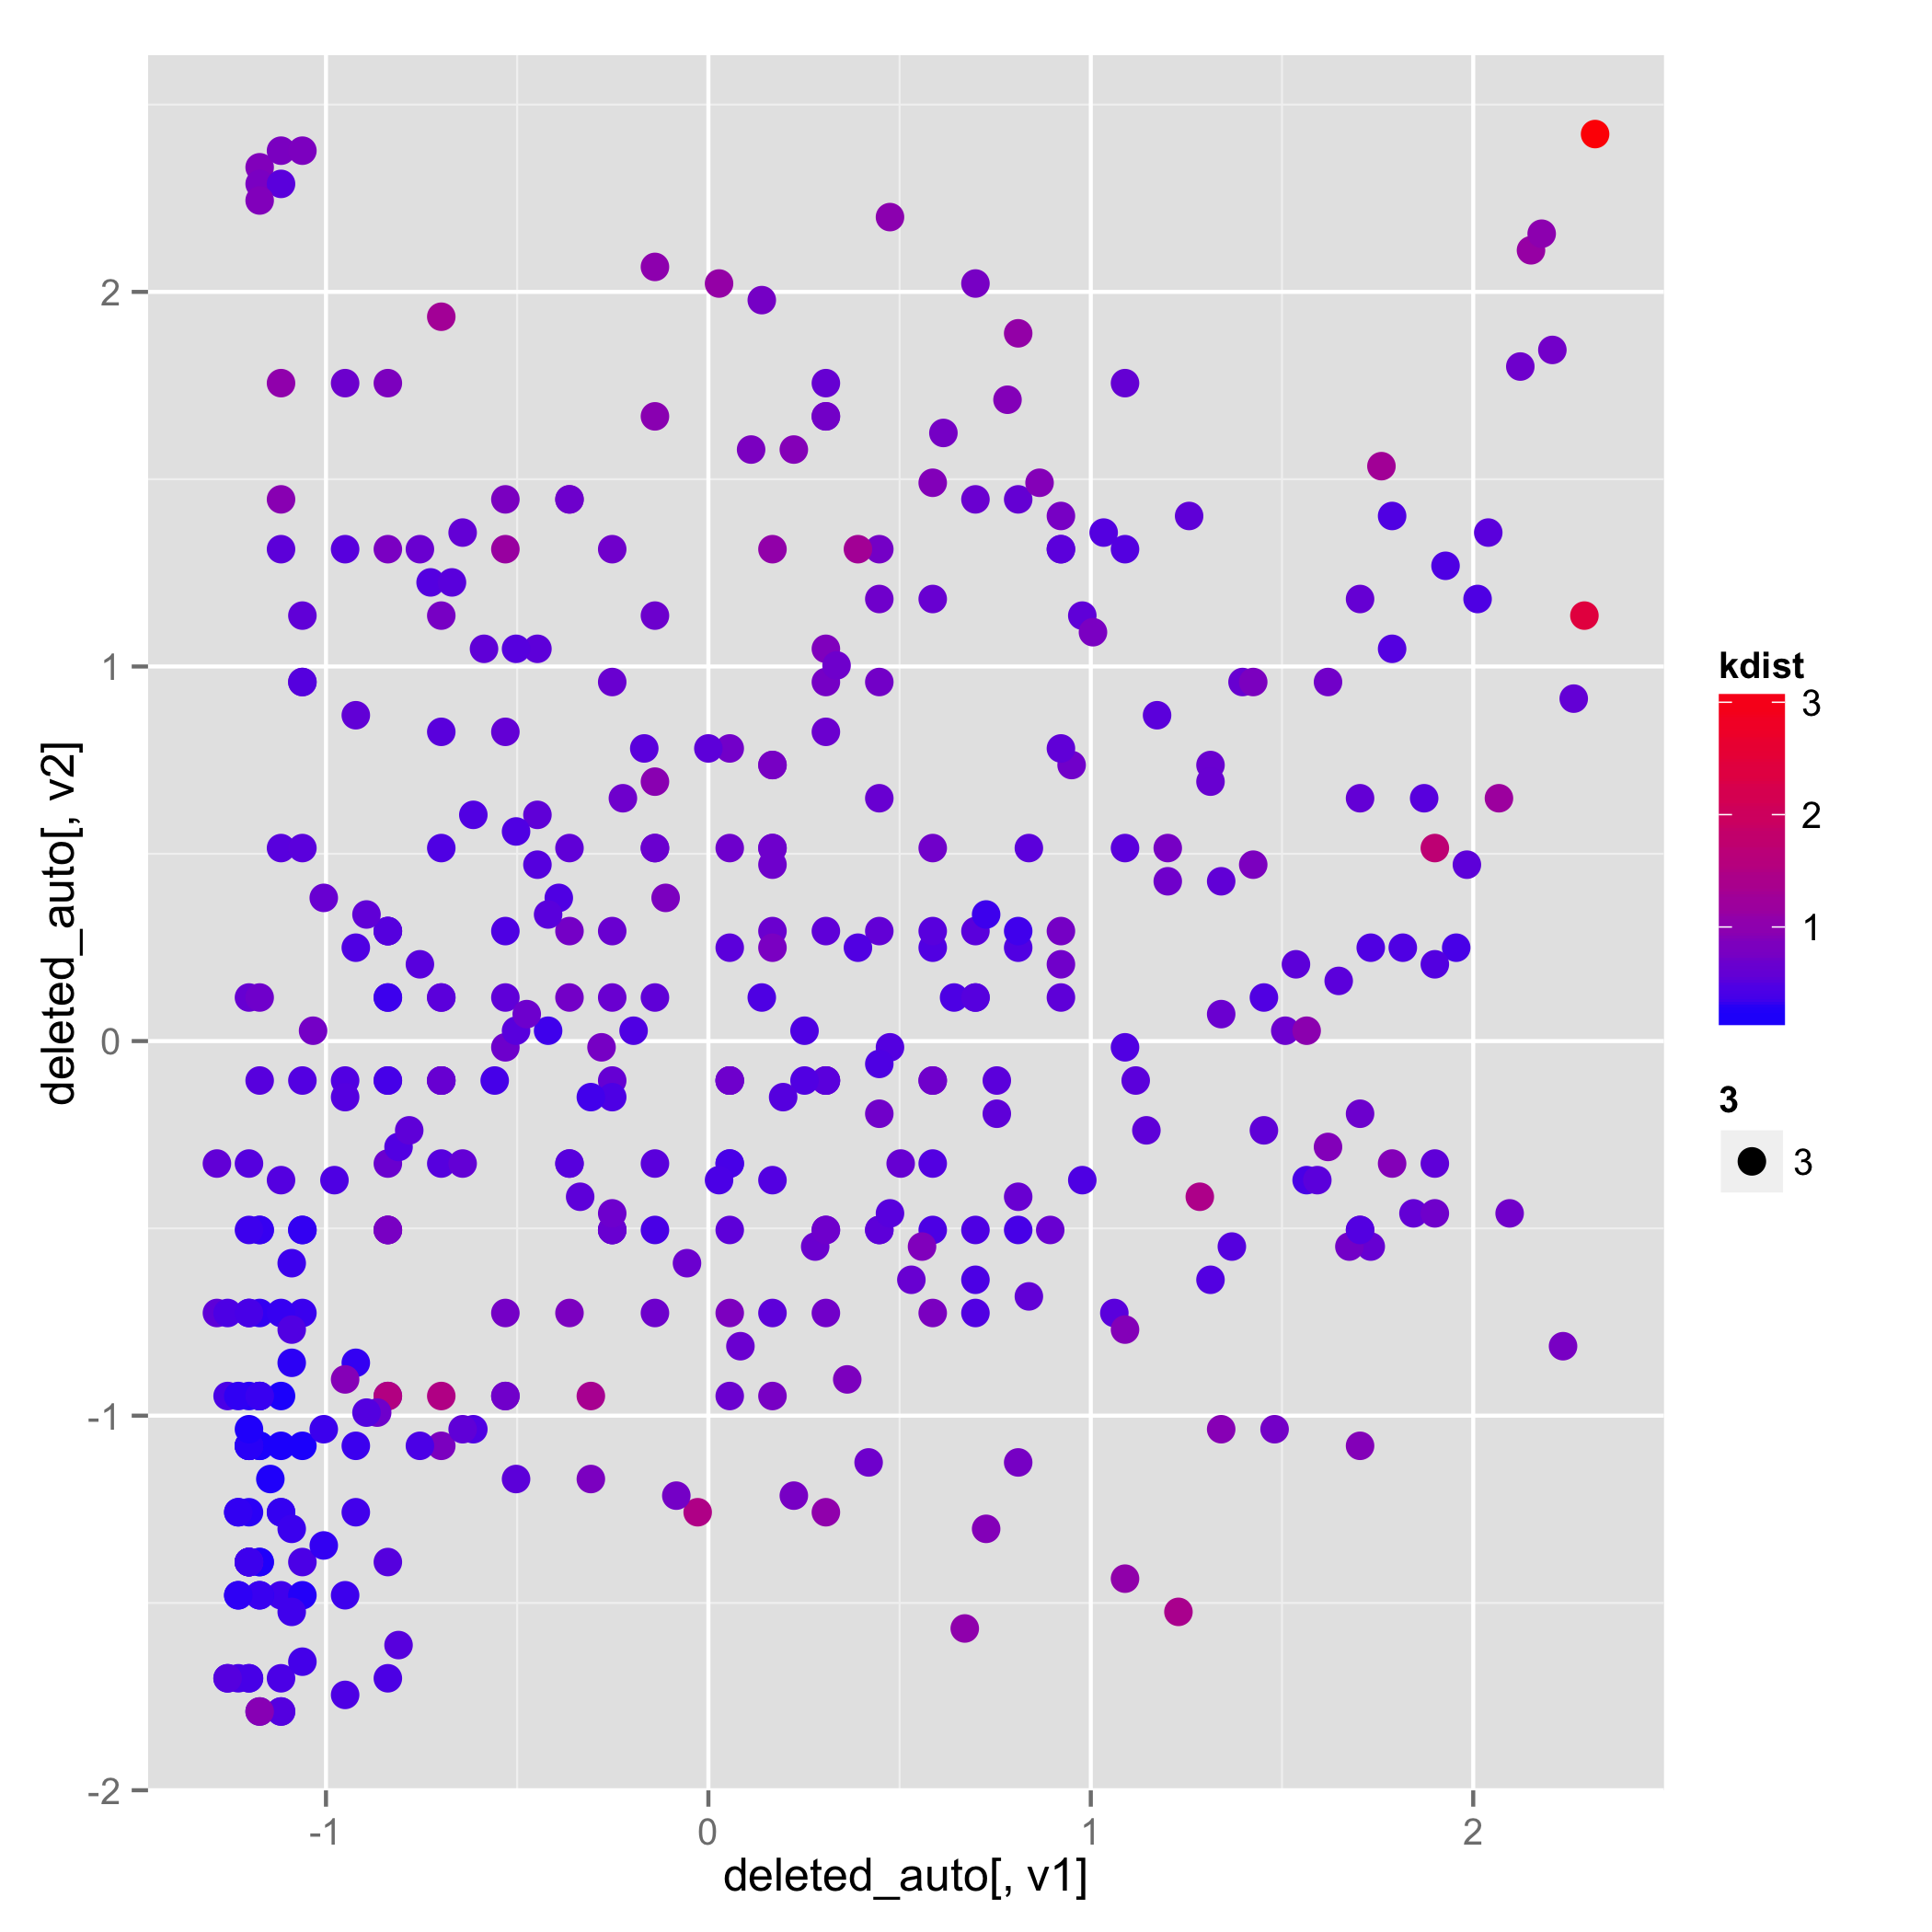
\includegraphics[scale=0.05]{using_kdist1_6.png}
\par\end{centering}}
\quad{}
\subfloat[]{\begin{centering}
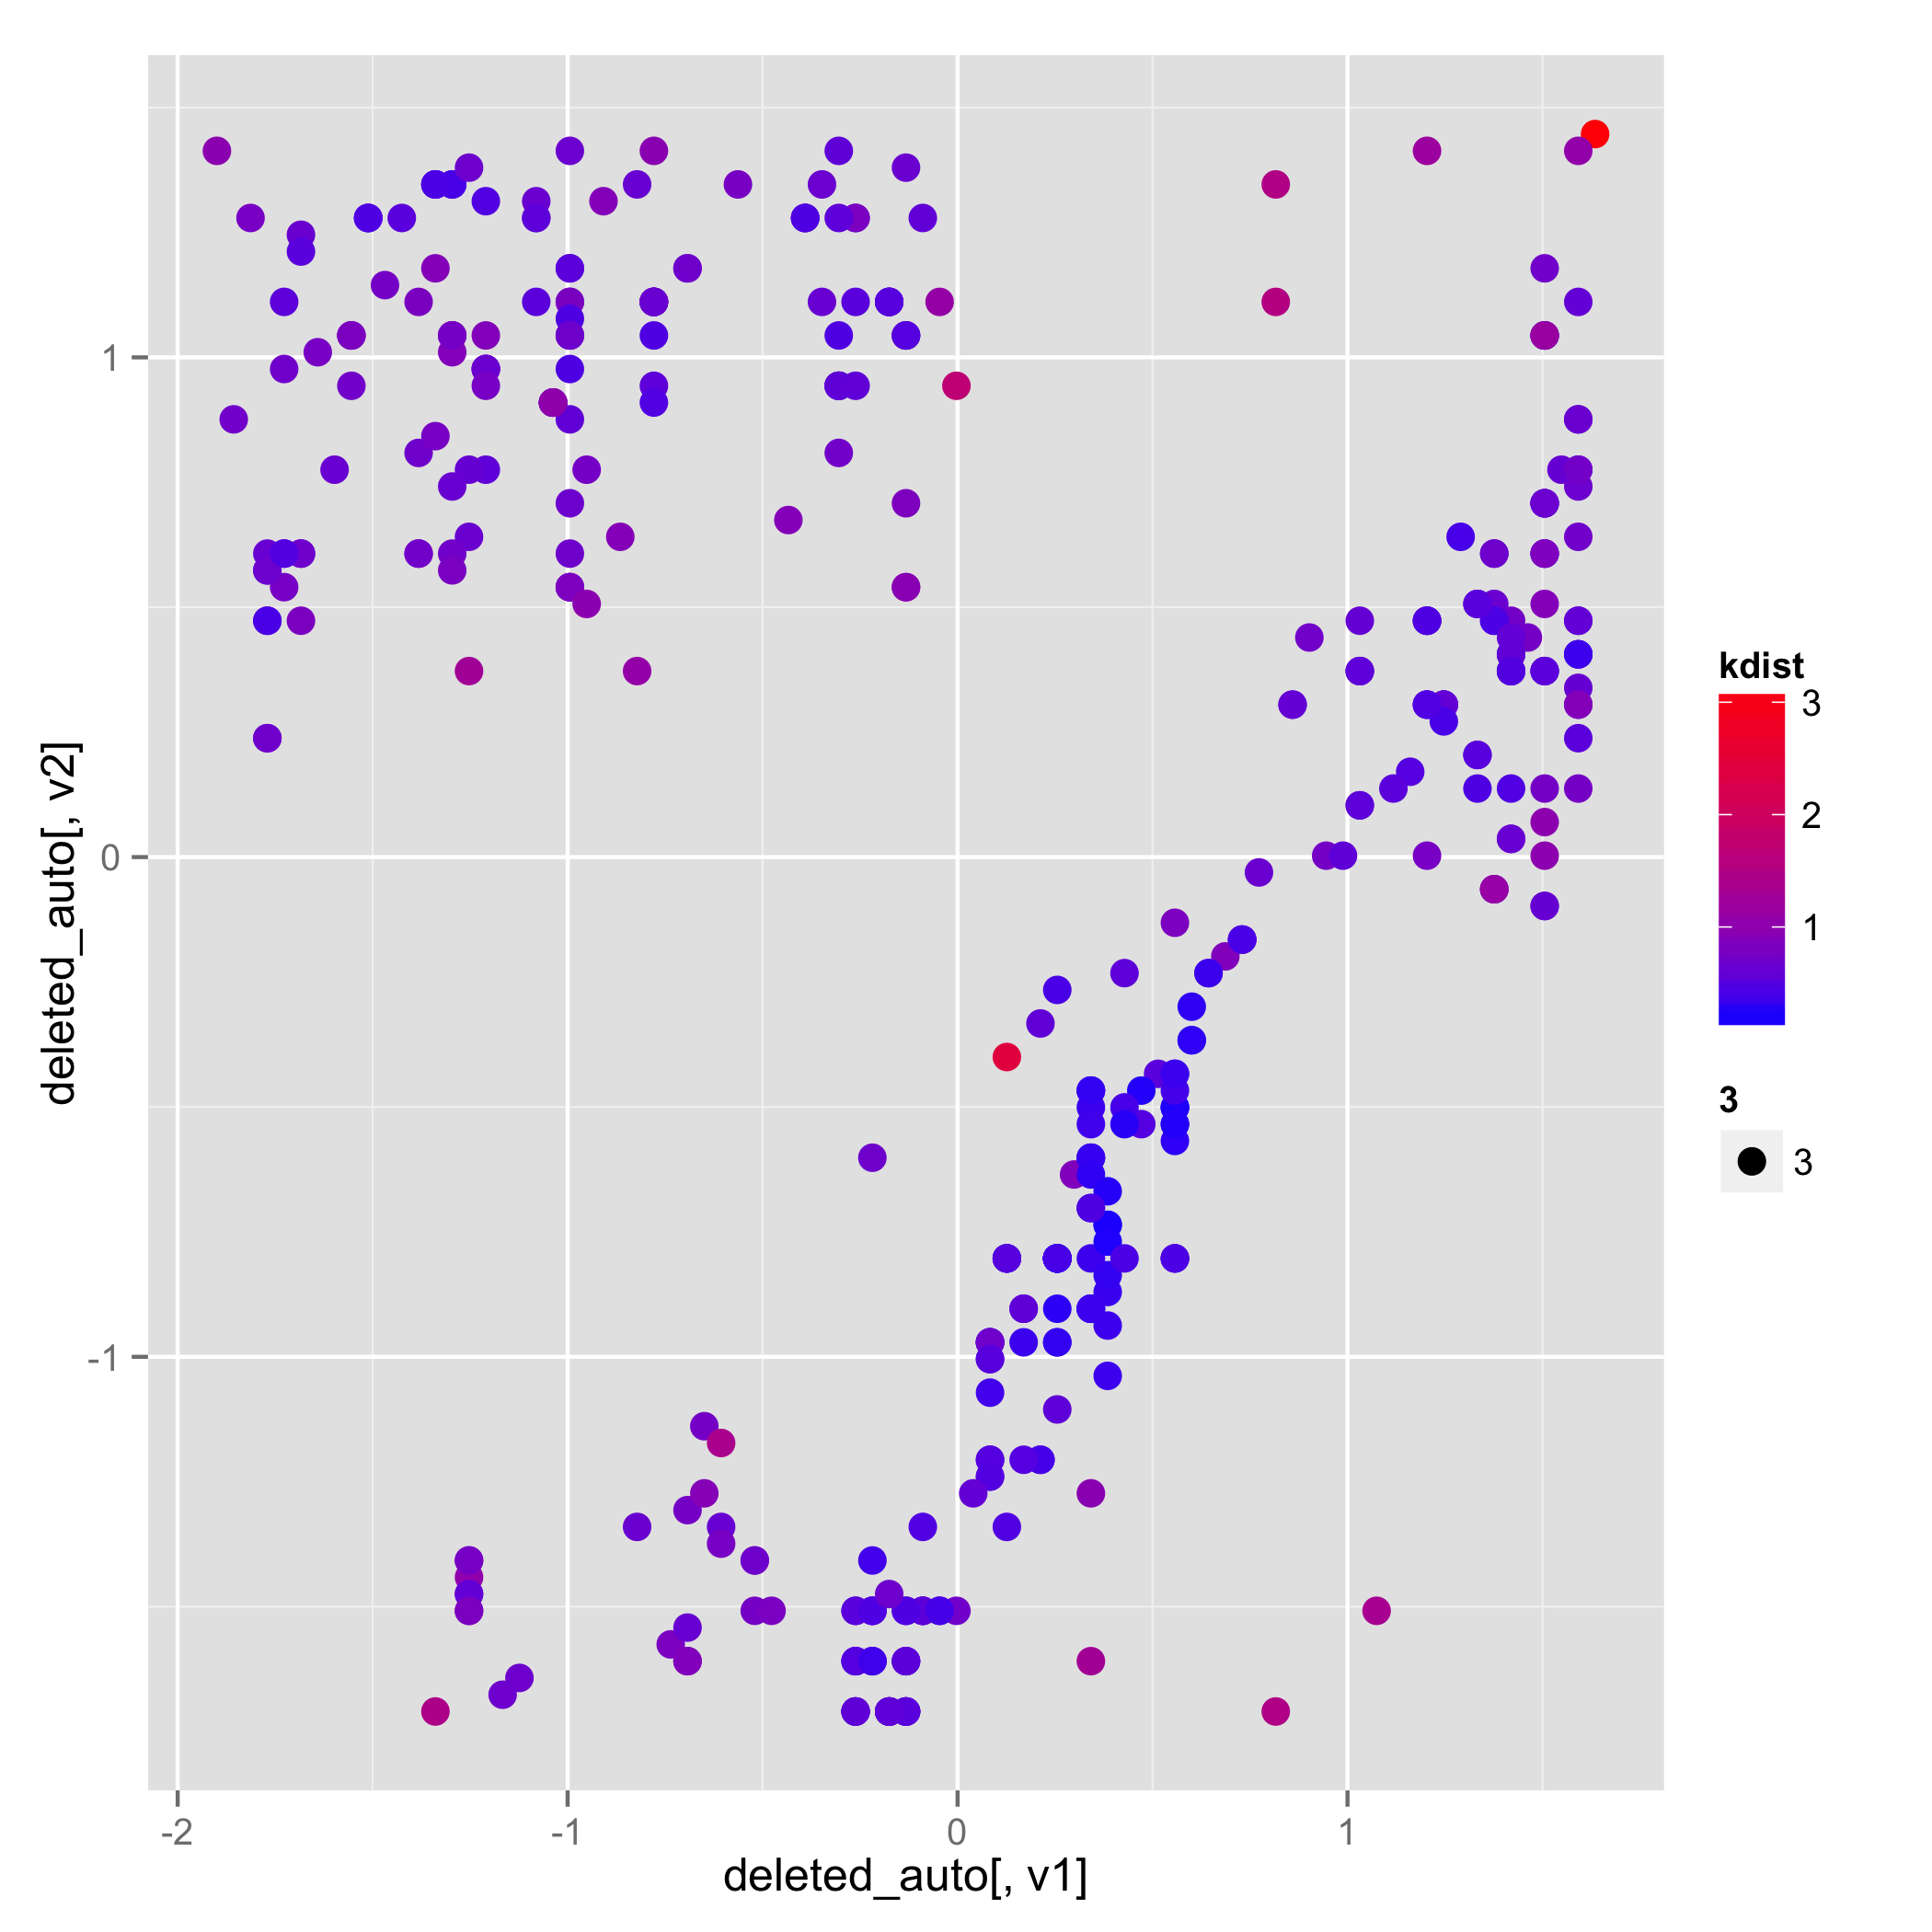
\includegraphics[scale=0.05]{using_kdist3_4.png}
\par\end{centering}}
\quad{}
\subfloat[]{\begin{centering}
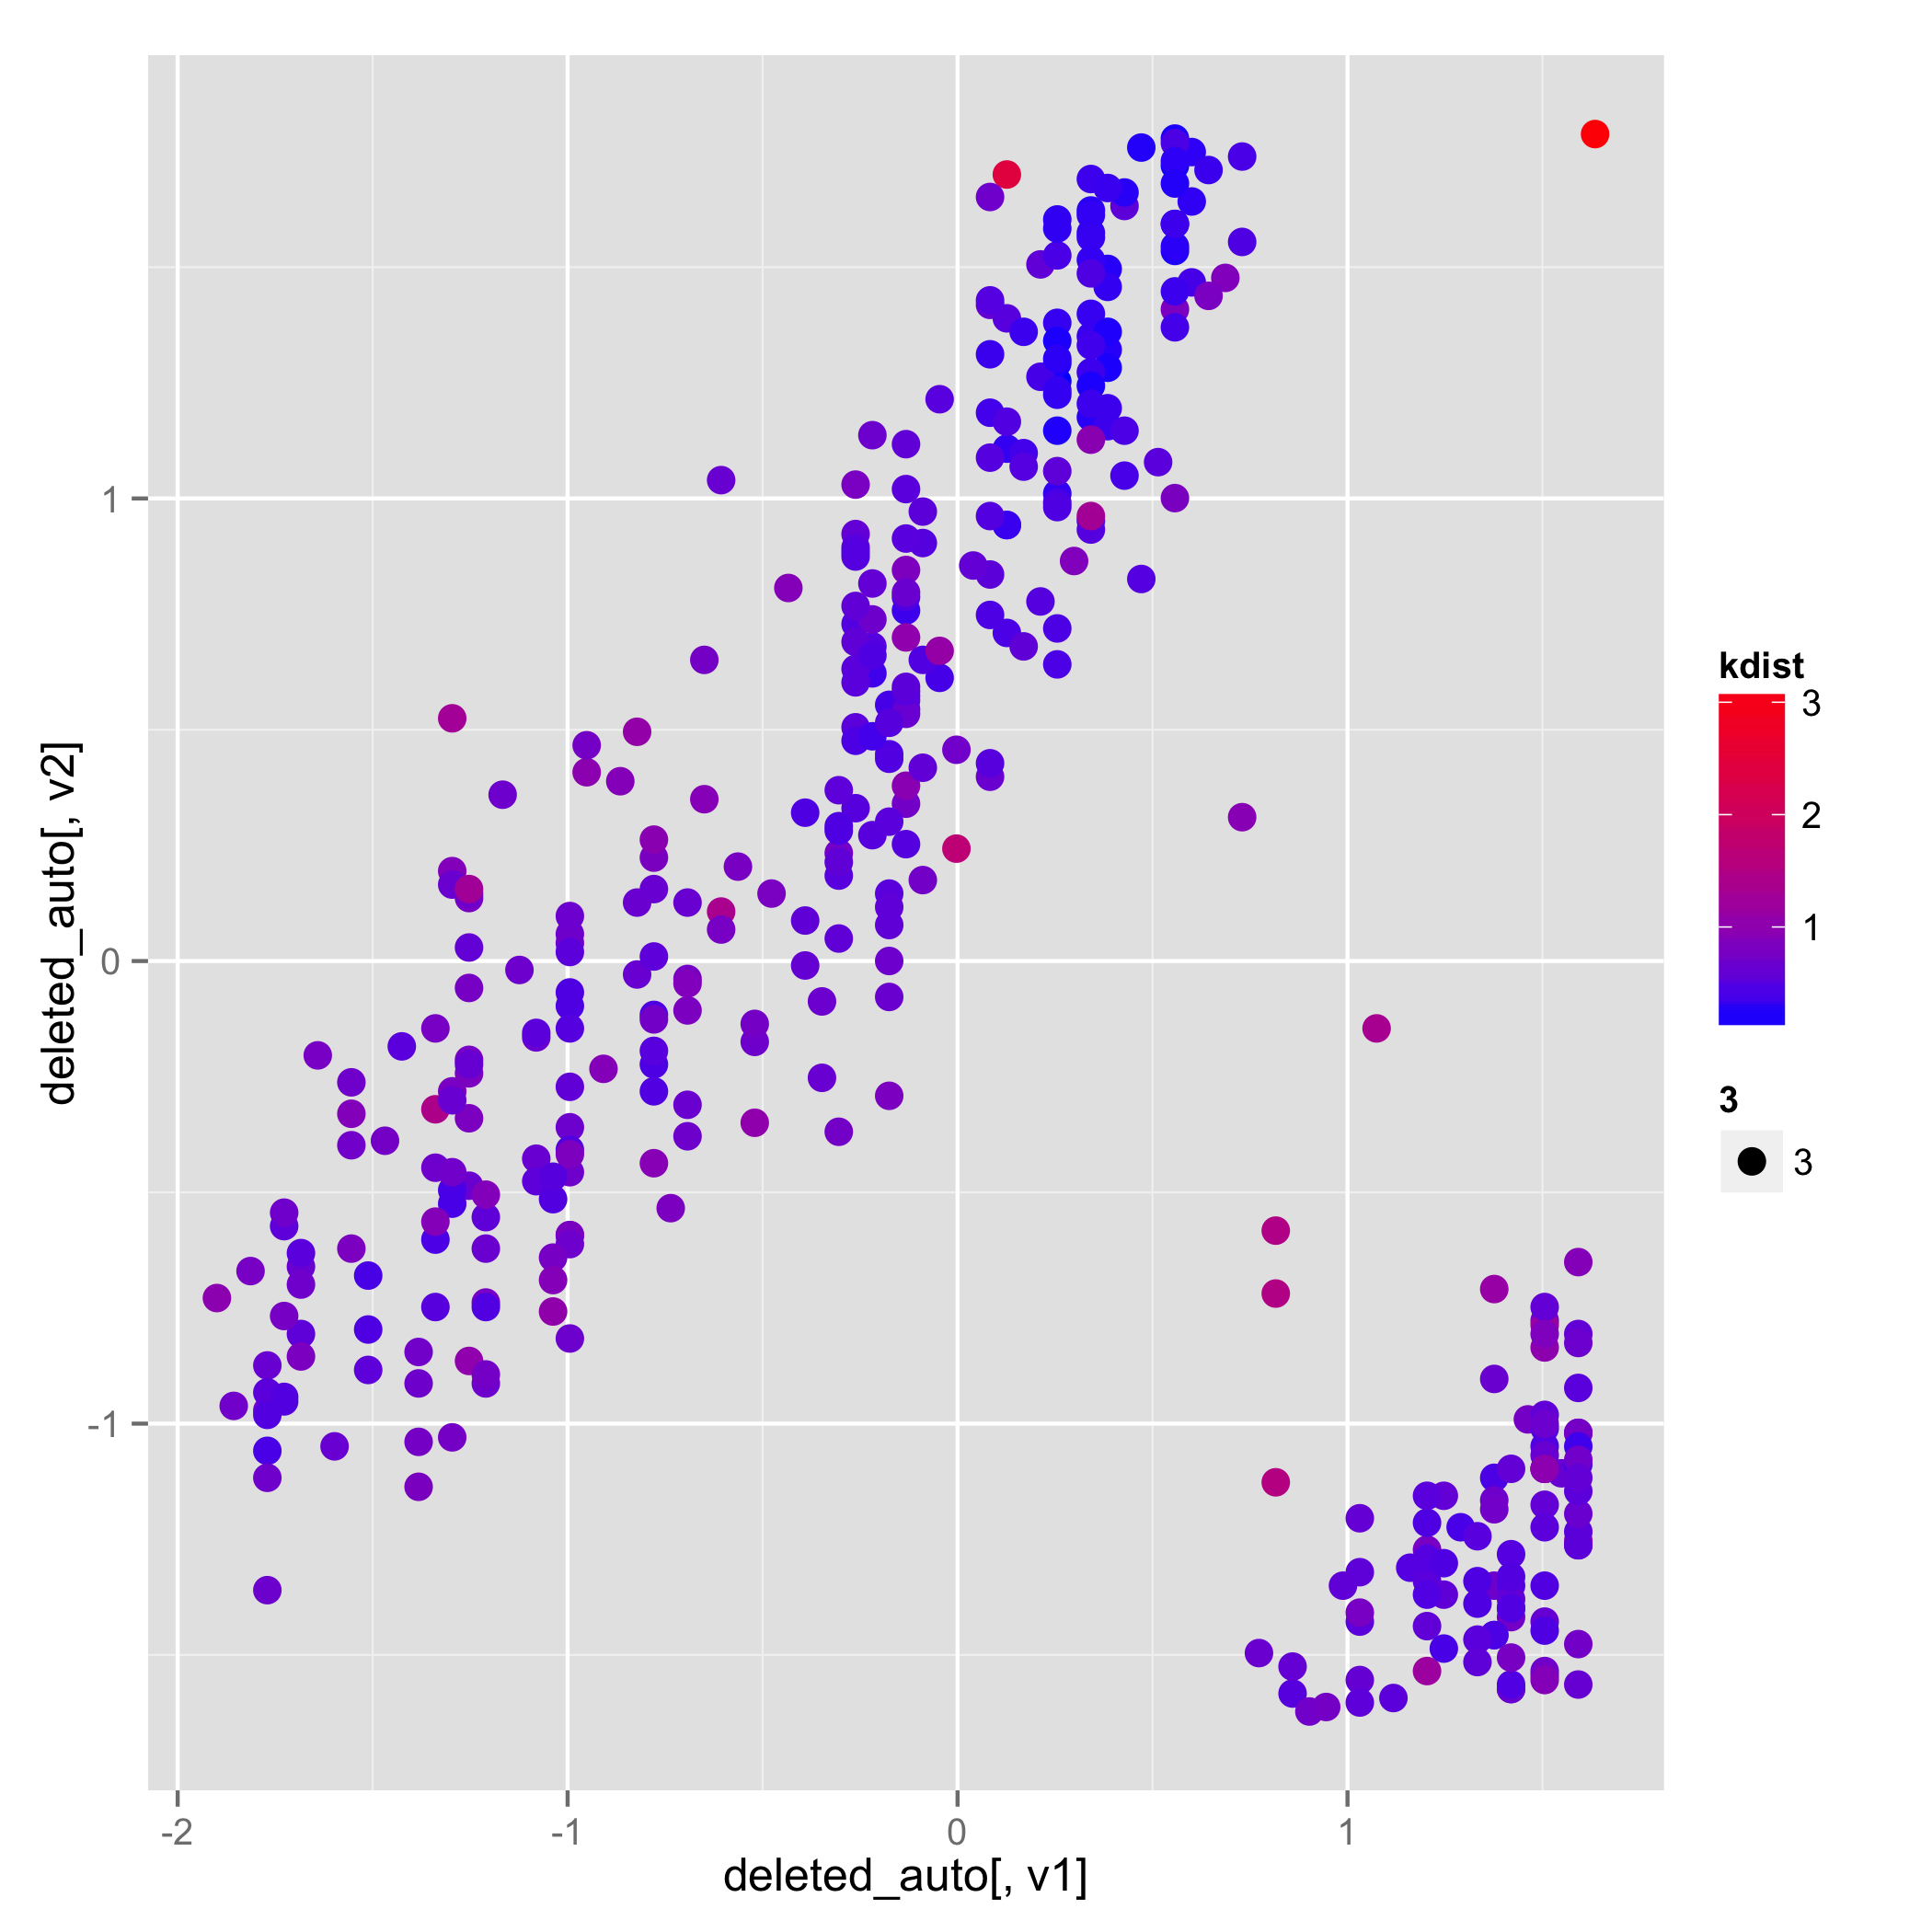
\includegraphics[scale=0.05]{using_kdist3_5.png}
\par\end{centering}}
\quad{}
\subfloat[]{\begin{centering}
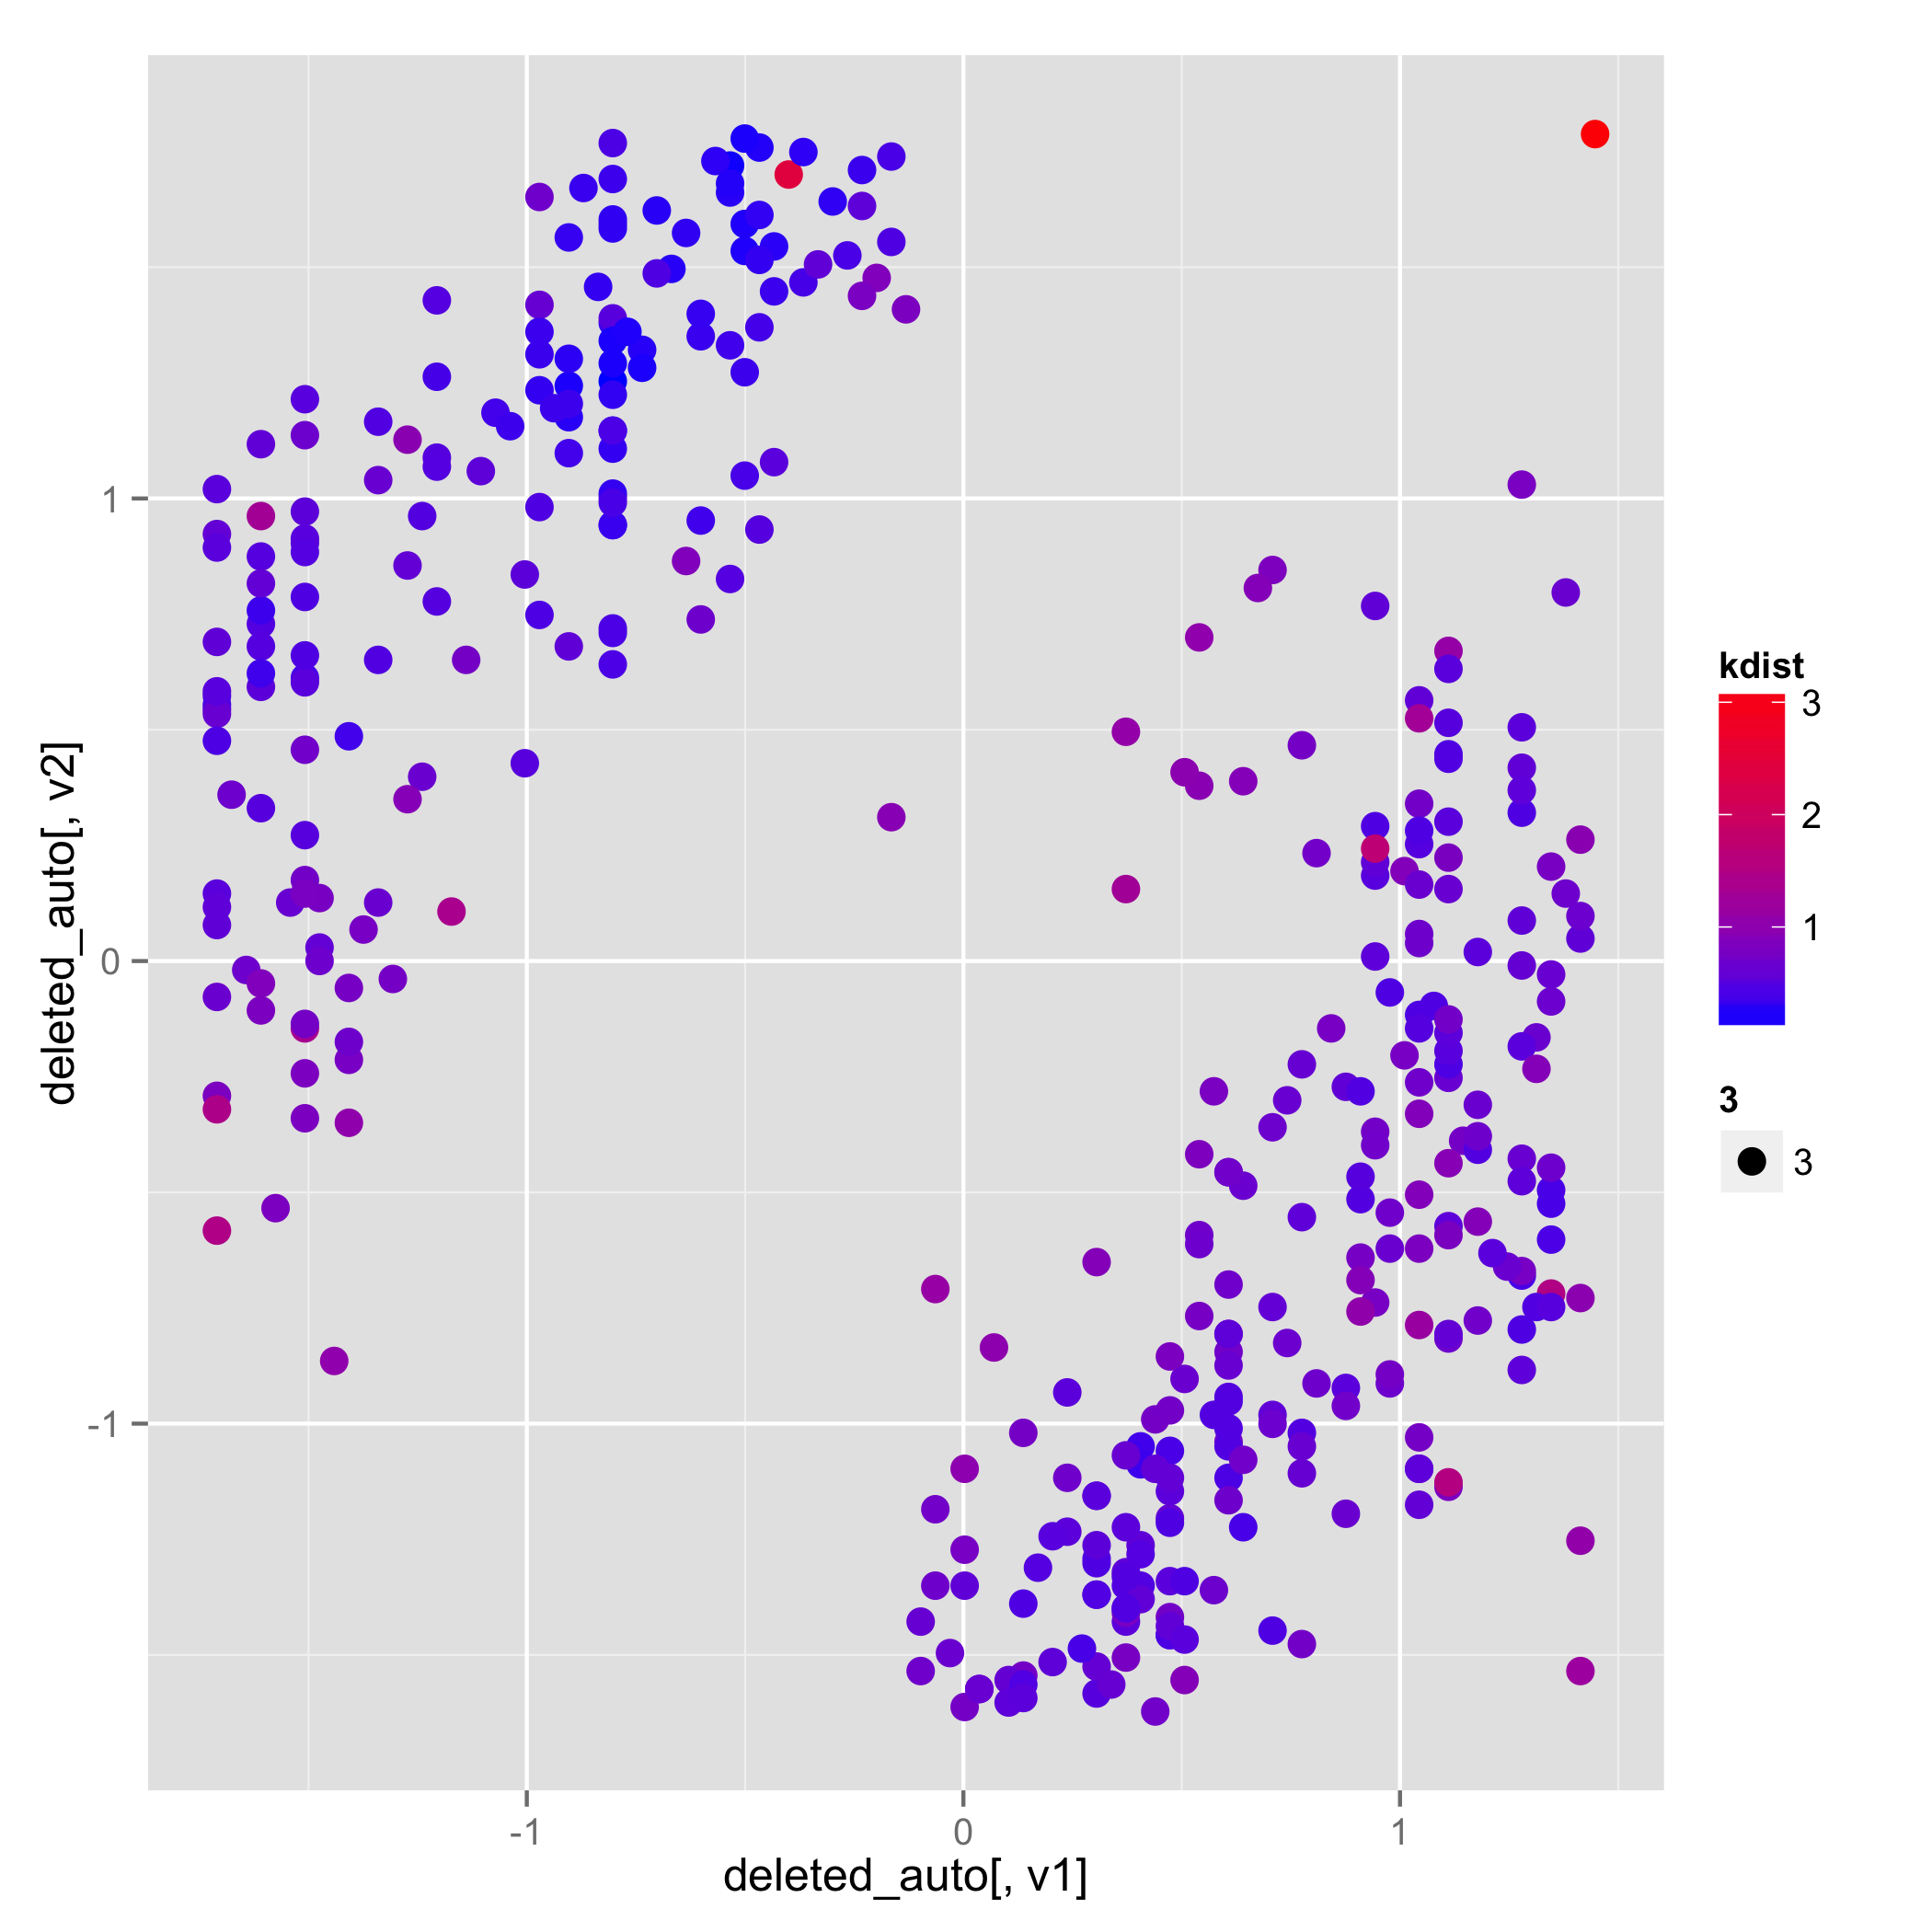
\includegraphics[scale=0.05]{using_kdist4_5.png}
\par\end{centering}}
\quad{}
\subfloat[]{\begin{centering}
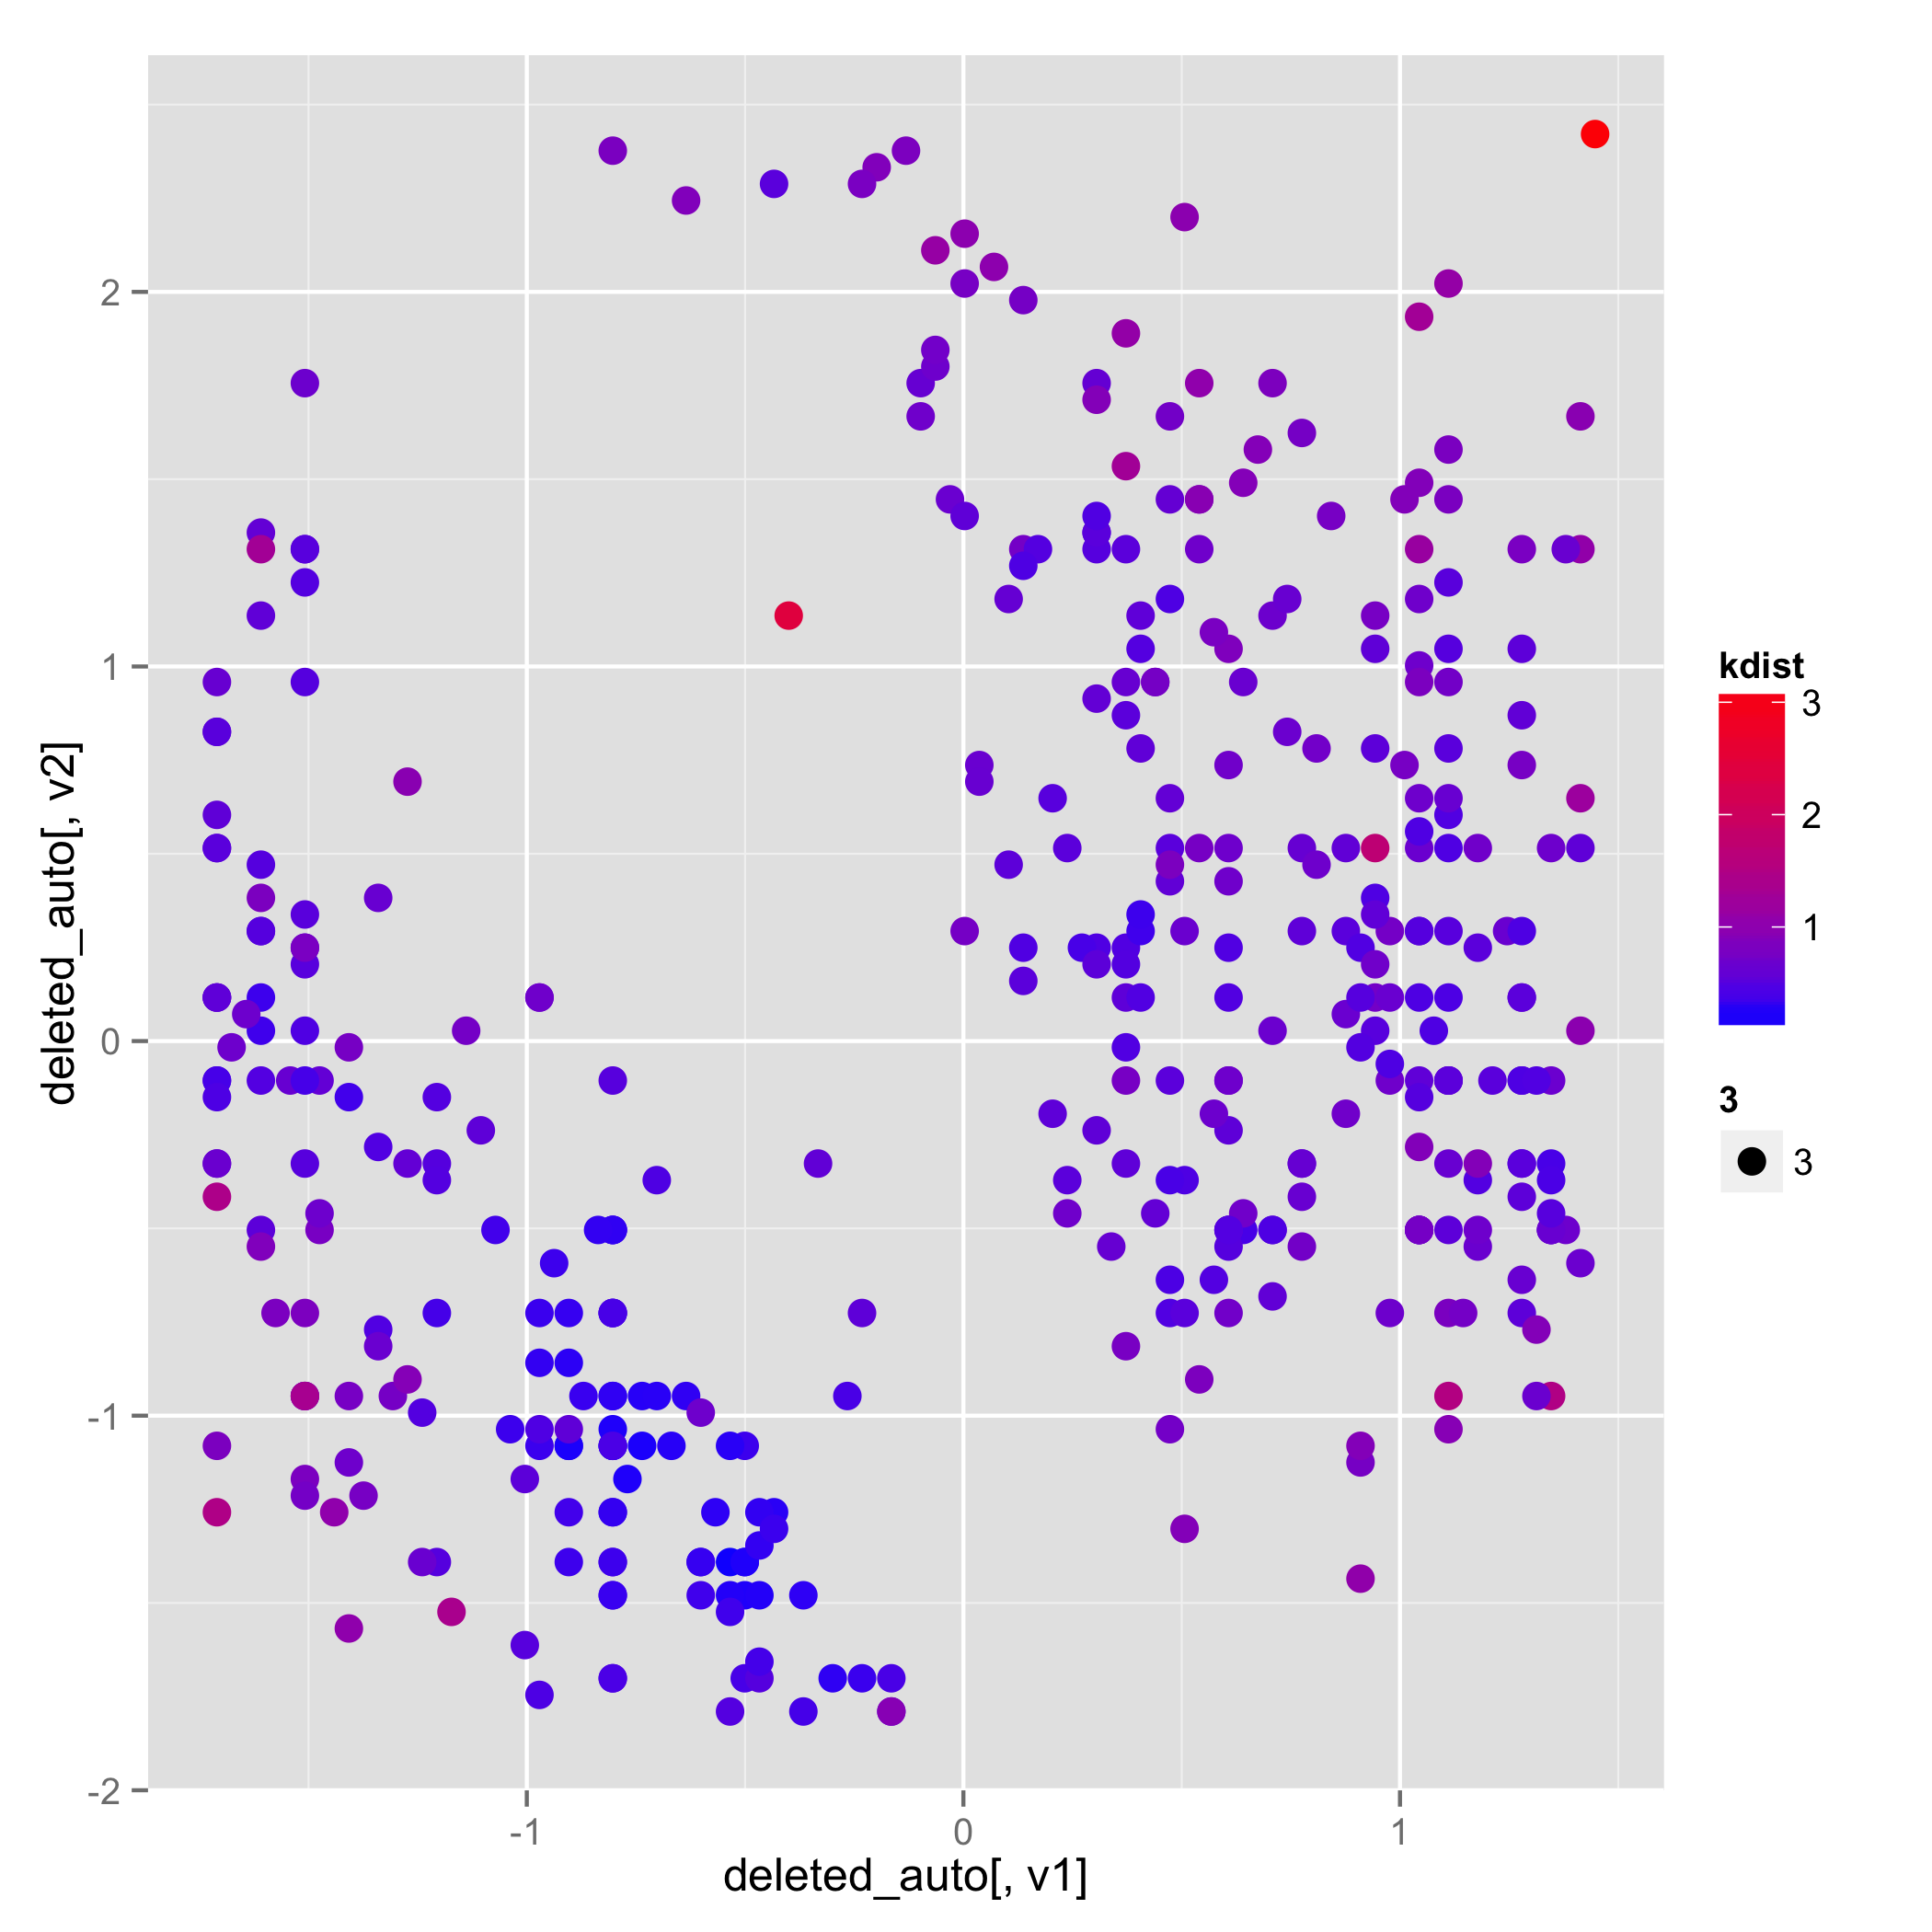
\includegraphics[scale=0.05]{using_kdist4_6.png}
\par\end{centering}}
\quad{}
\subfloat[]{\begin{centering}
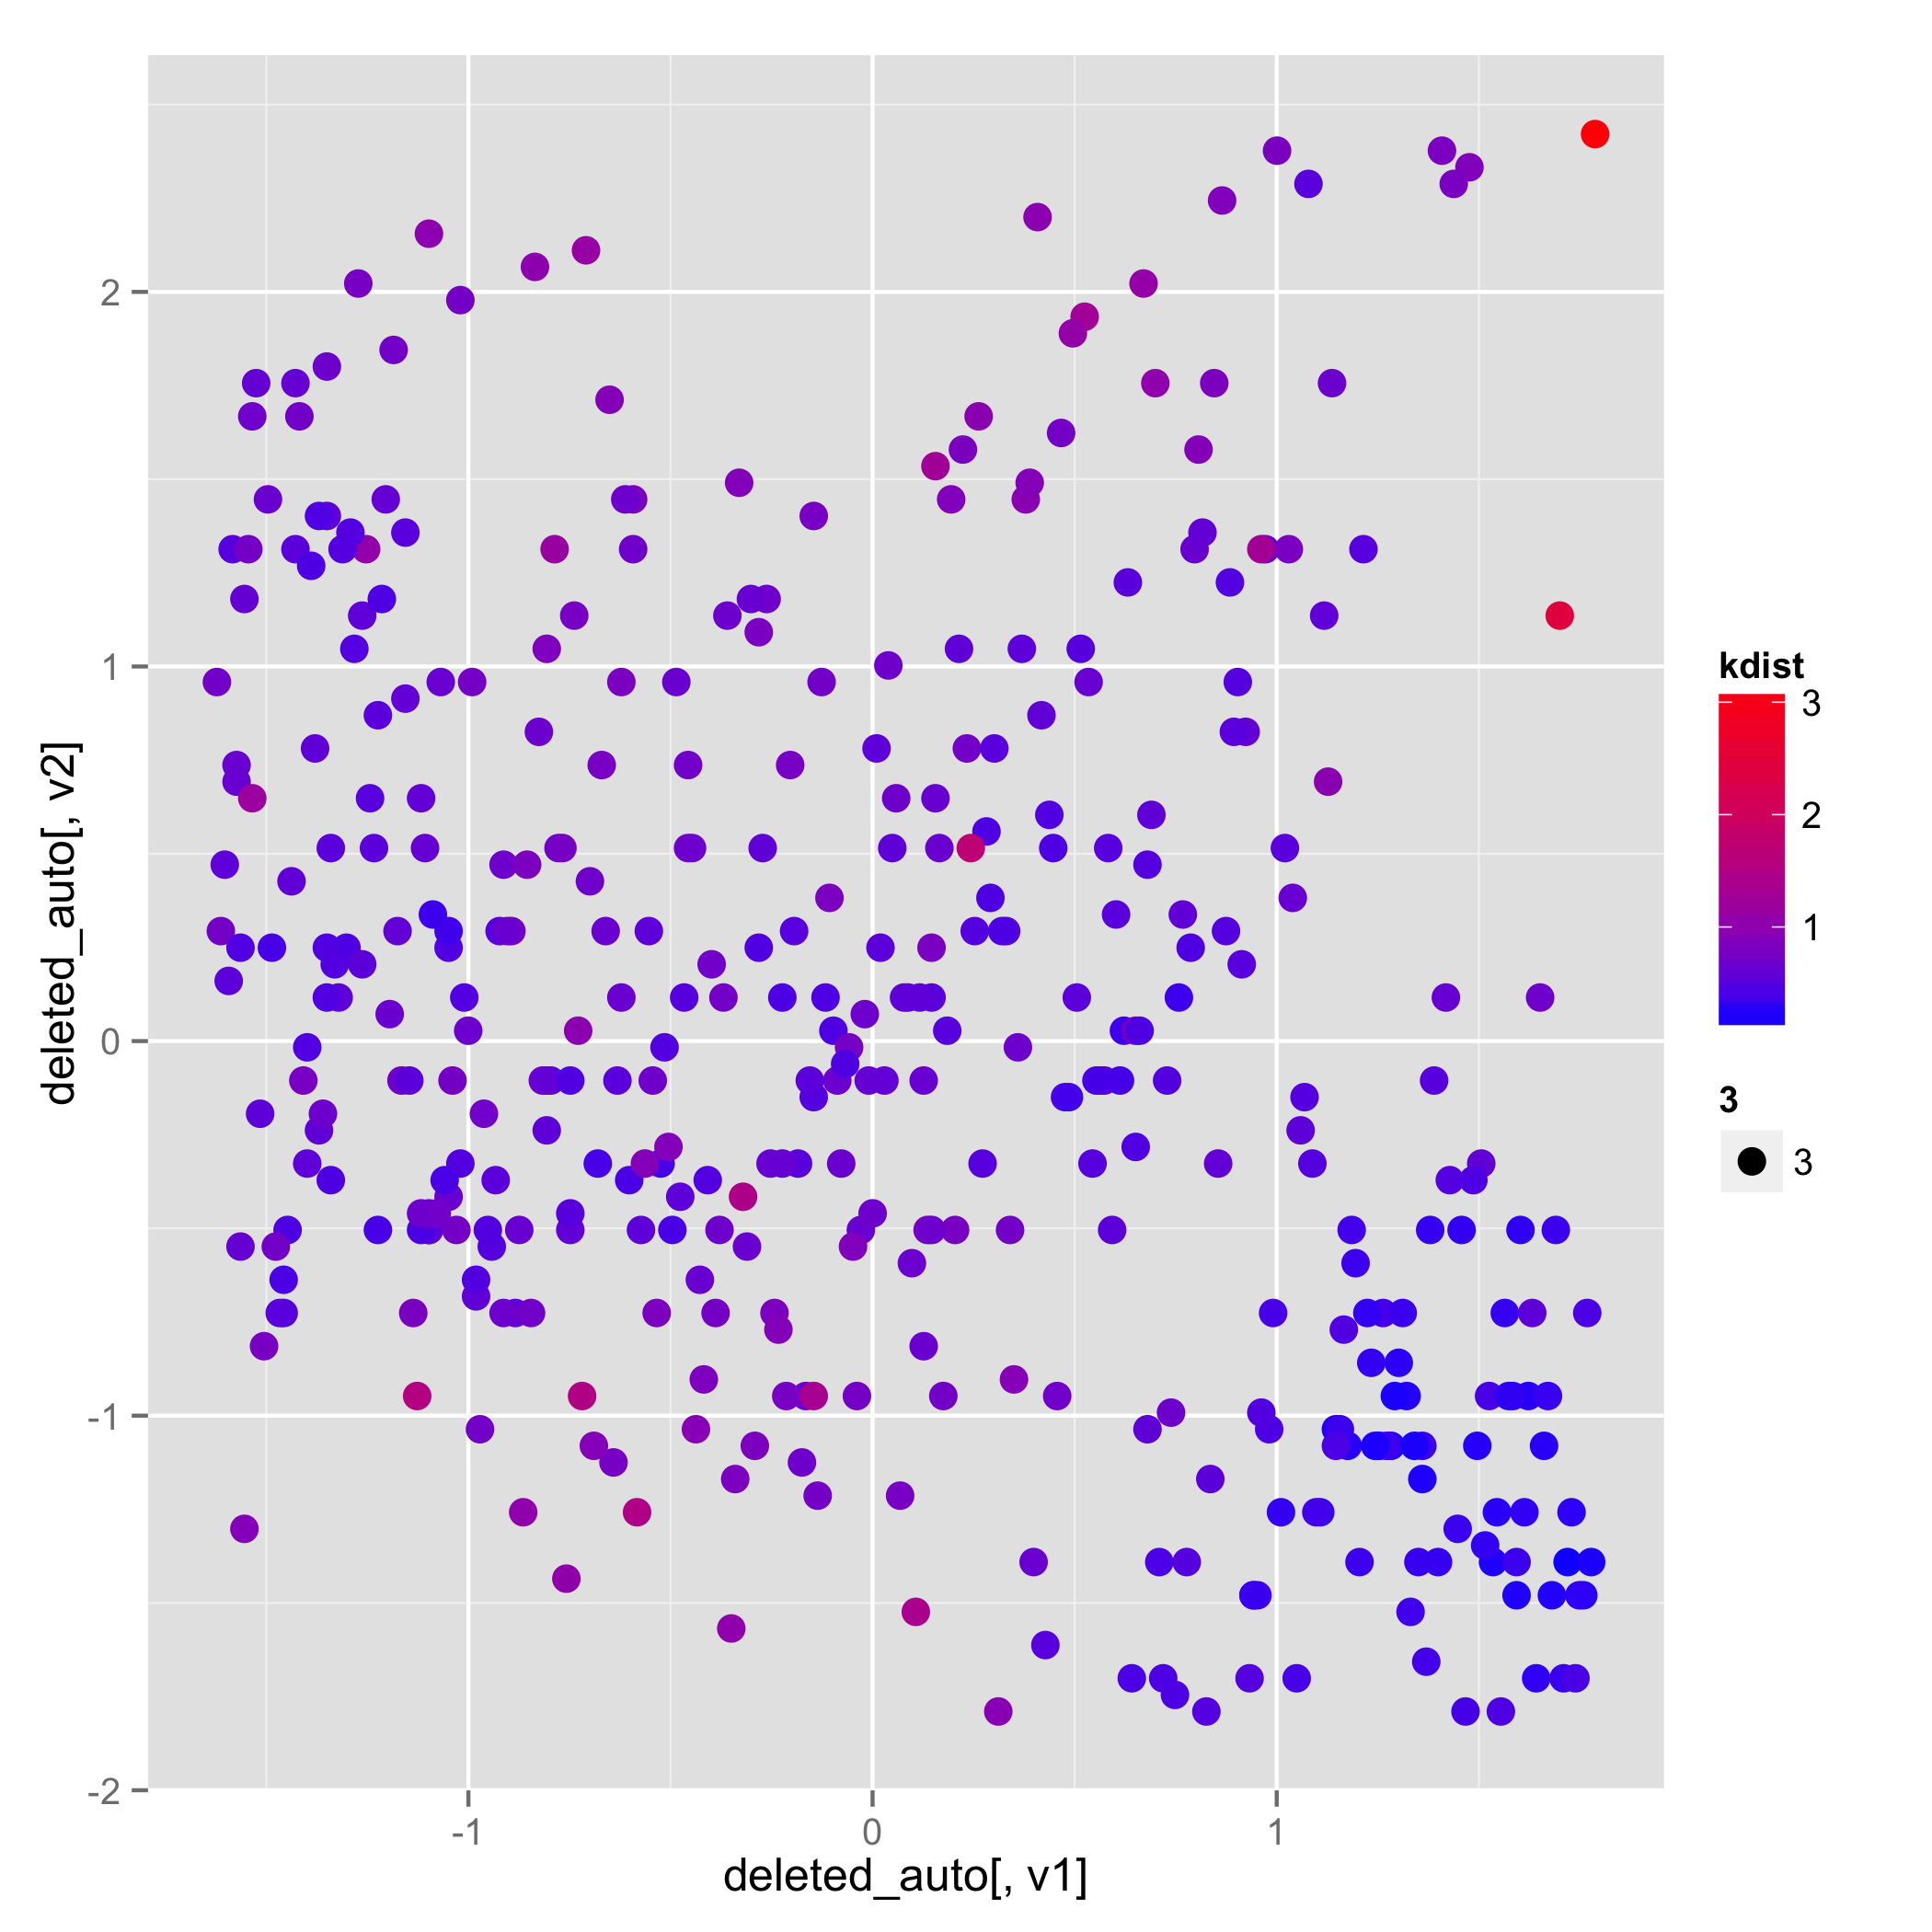
\includegraphics[scale=0.05]{using_kdist5_6.png}
\par\end{centering}}
\end{center}
\end{figure}


\item Using density as a metric, there are 3 likely cutoff points. 
The three considered here are values of 1.8, 2.0, and 2.5. 

\begin{center}
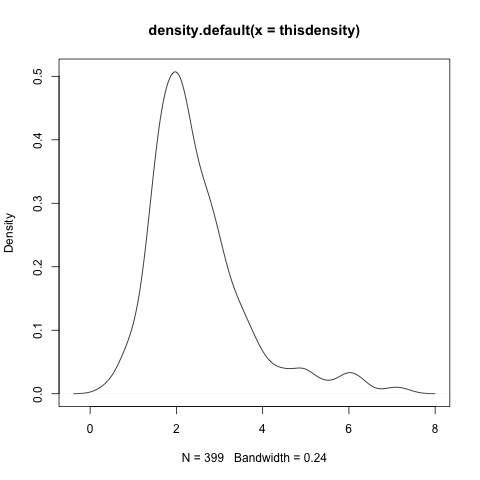
\includegraphics[scale=0.35]{density_density}
\end{center}

    %# density:
%    thisdensity = my.density(deleted_auto[,cols],5)
%    plot(density(thisdensity))
%    (1:nrow(deleted_auto))[thisdensity>=5]
%41  42  43  44  45  46  65  66  67  70  71  89  94 117 158 190 192 210
%    (1:nrow(deleted_auto))[thisdensity>=5.5]
%41  43  44  45  46  65  66  67  70  89 117 190 192 210


\begin{figure}[H]
\begin{center}
\subfloat[]{\begin{centering}
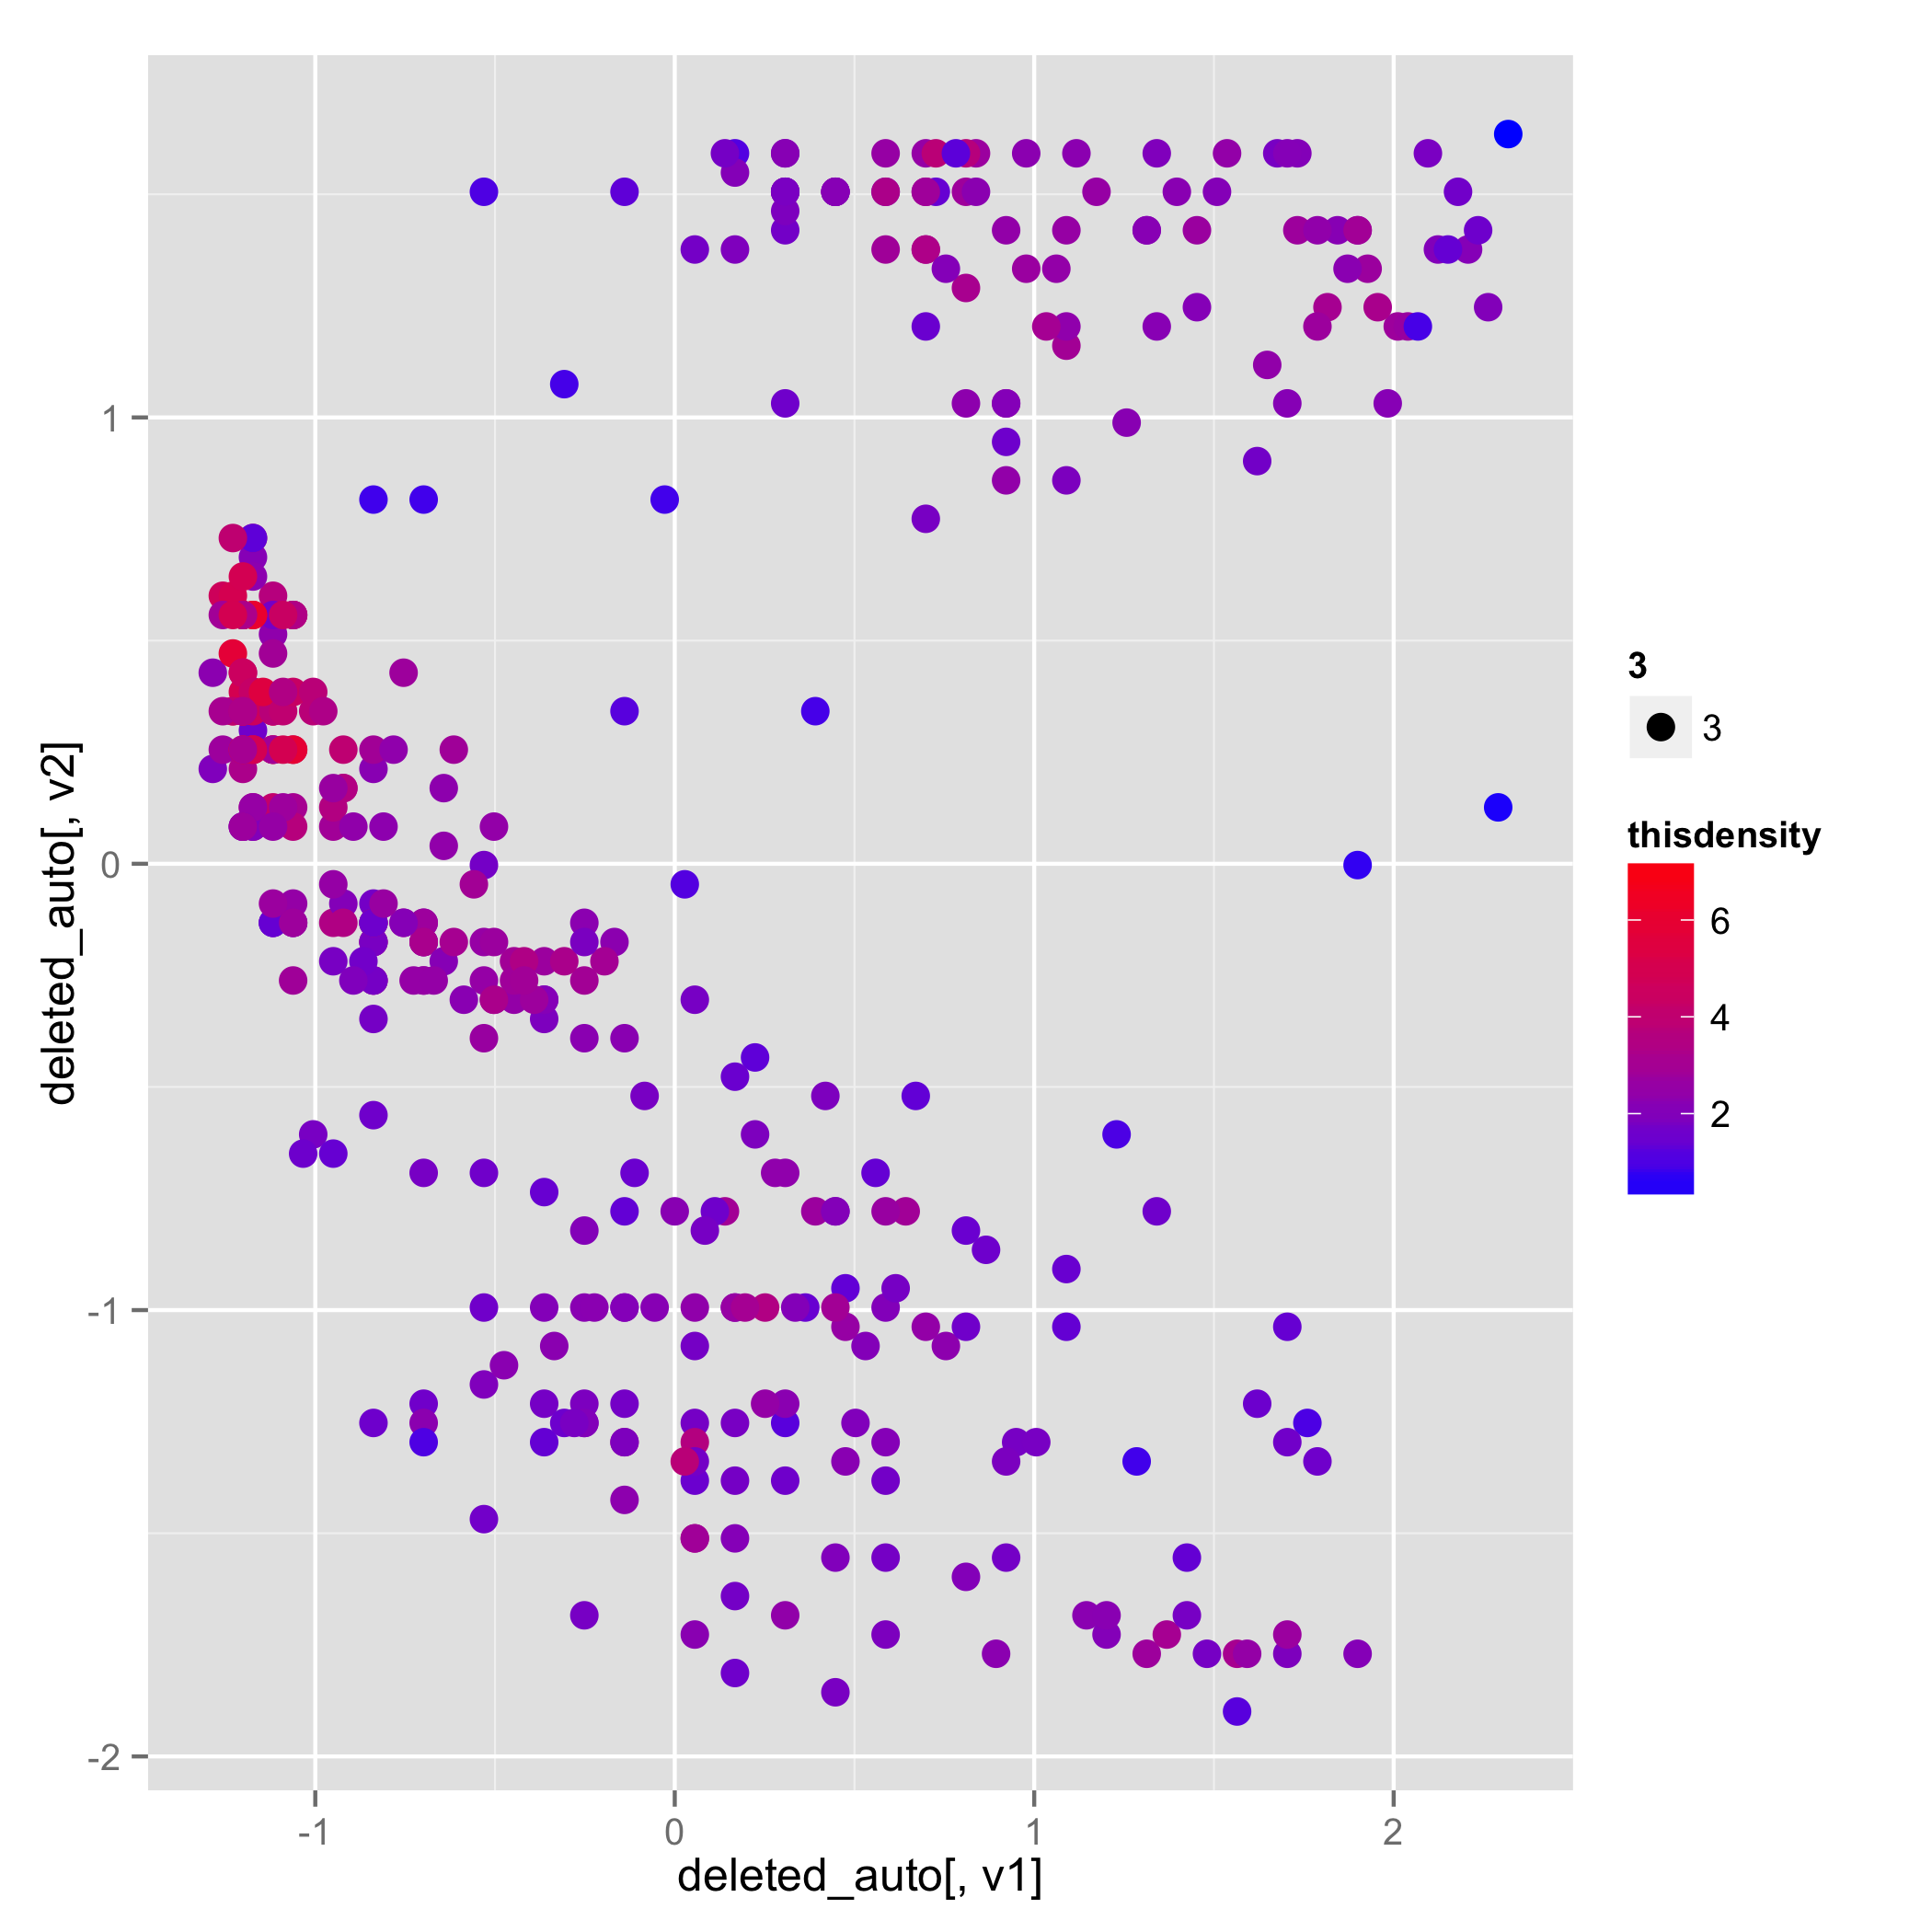
\includegraphics[scale=0.05]{using_density1_3.png}
\par\end{centering}}
\quad{}
\subfloat[]{\begin{centering}
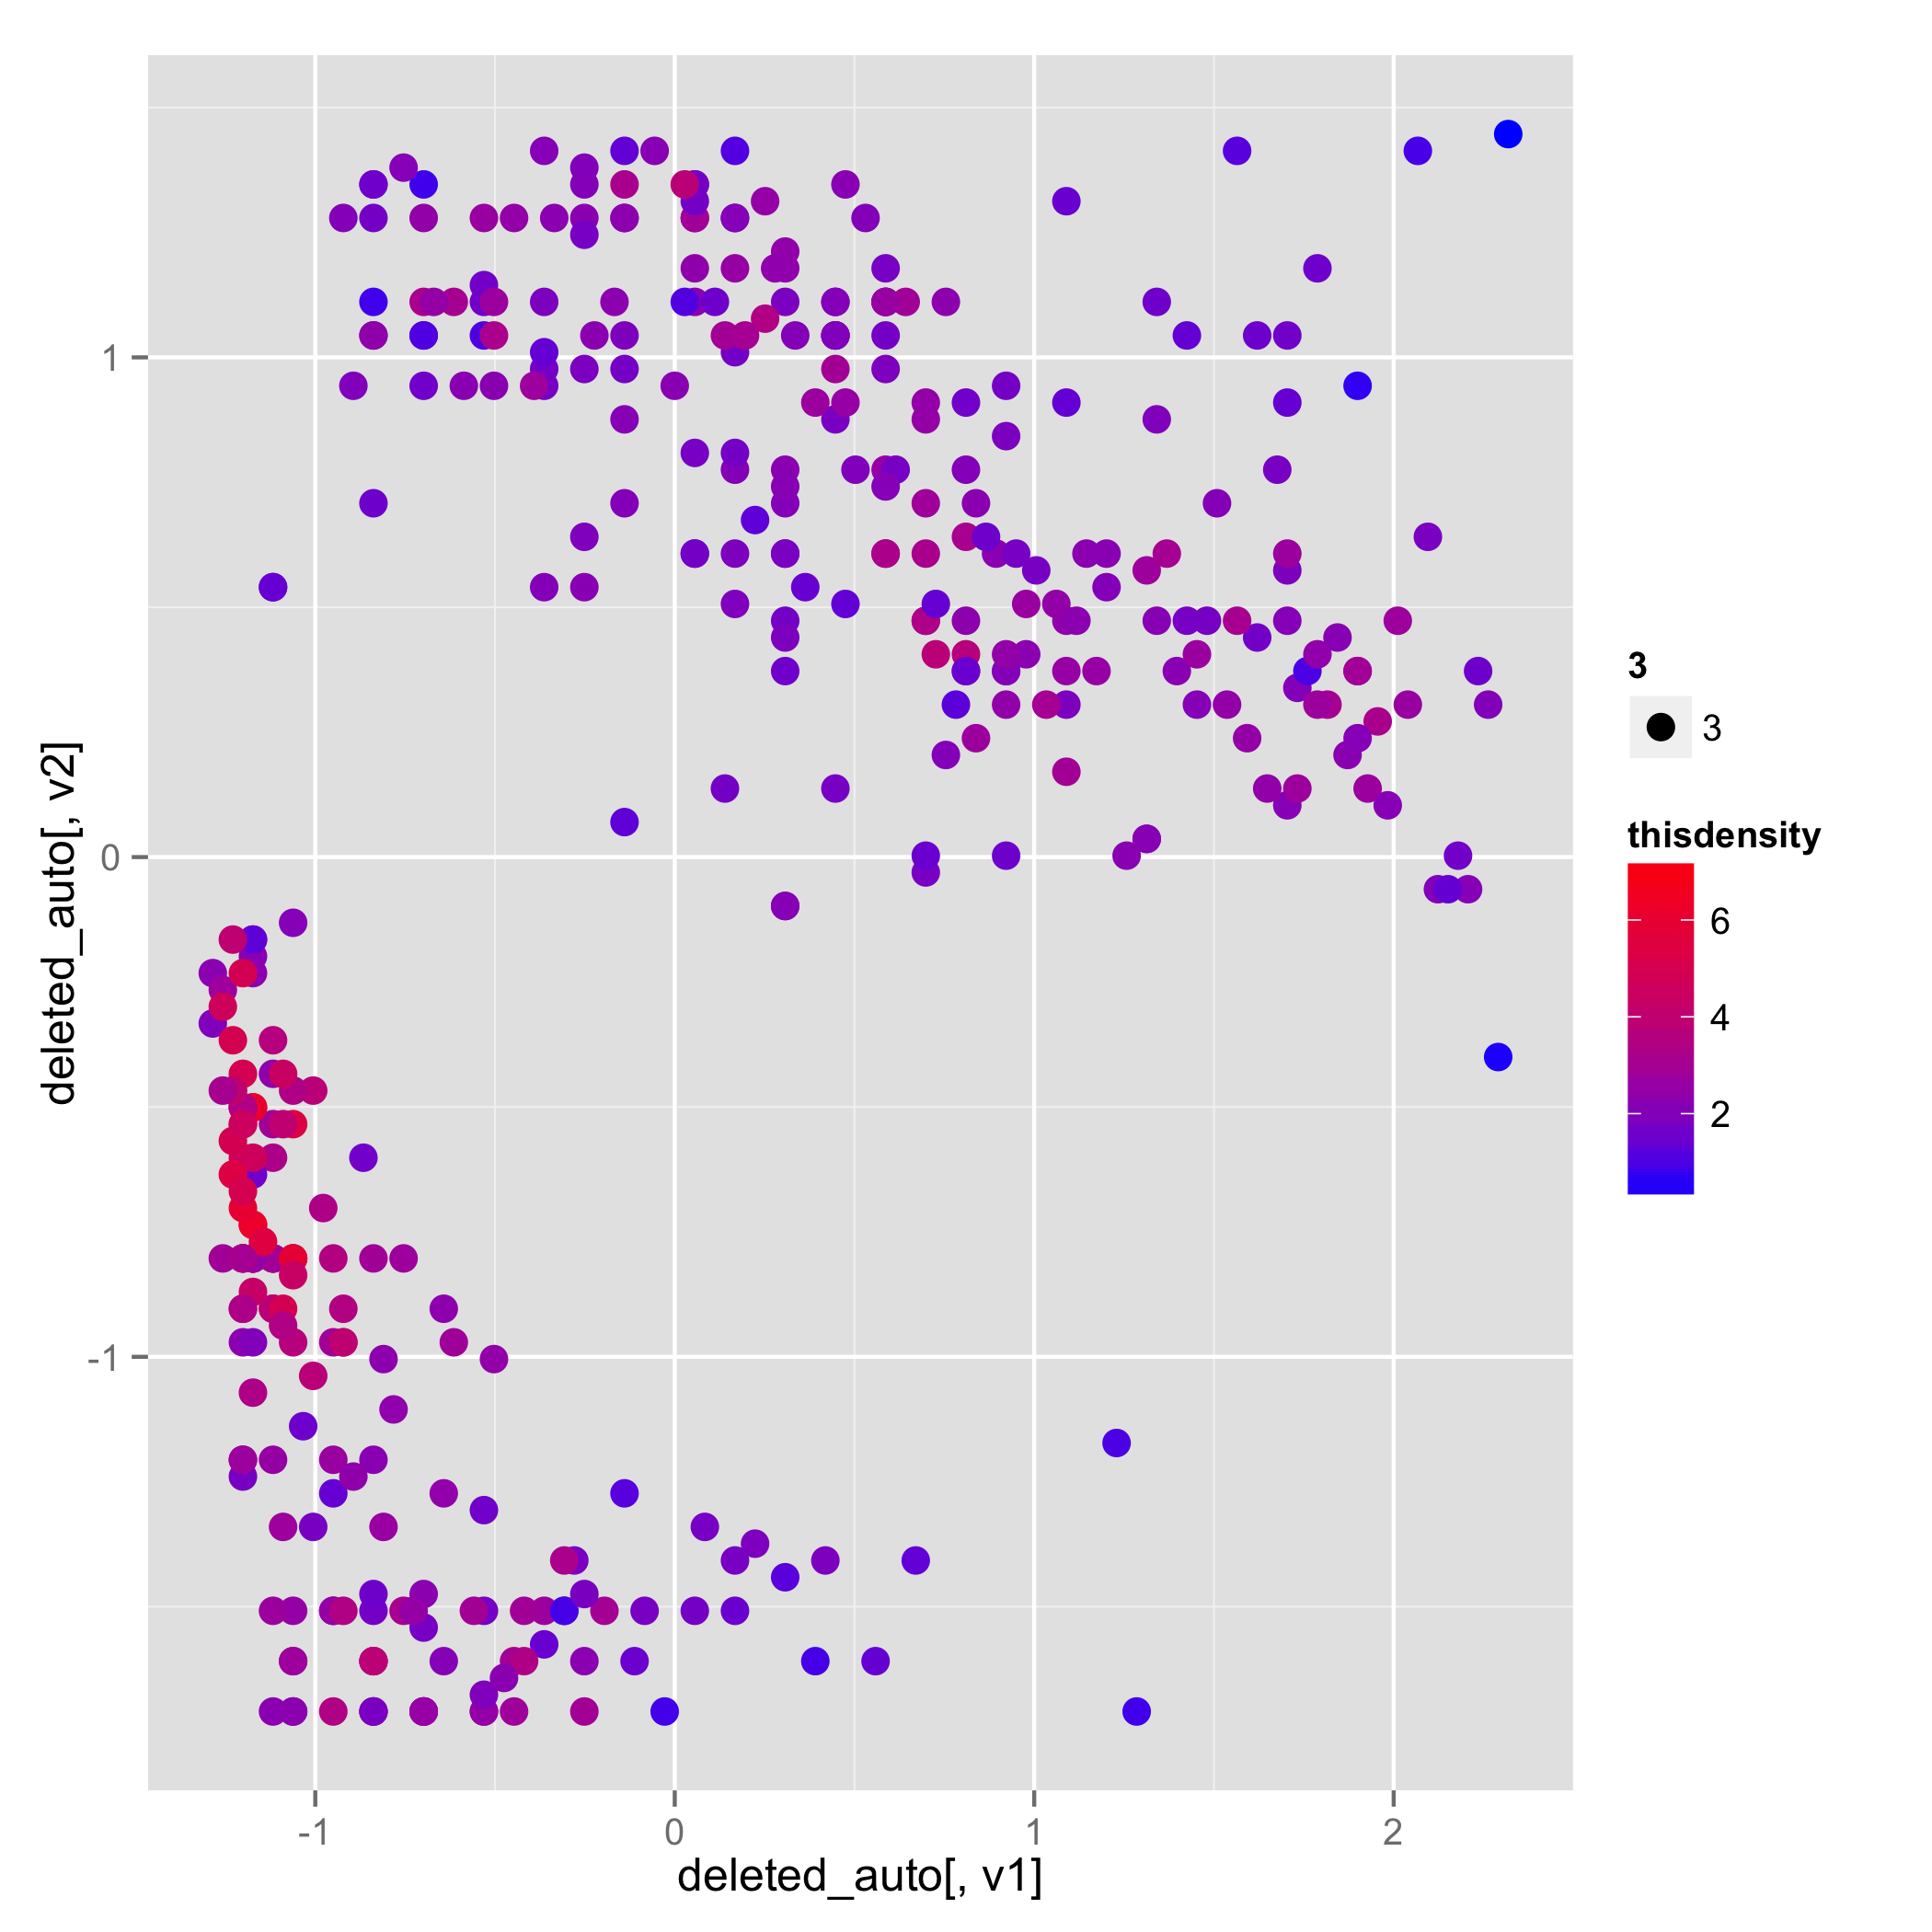
\includegraphics[scale=0.05]{using_density1_4.png}
\par\end{centering}}
\quad{}
\subfloat[]{\begin{centering}
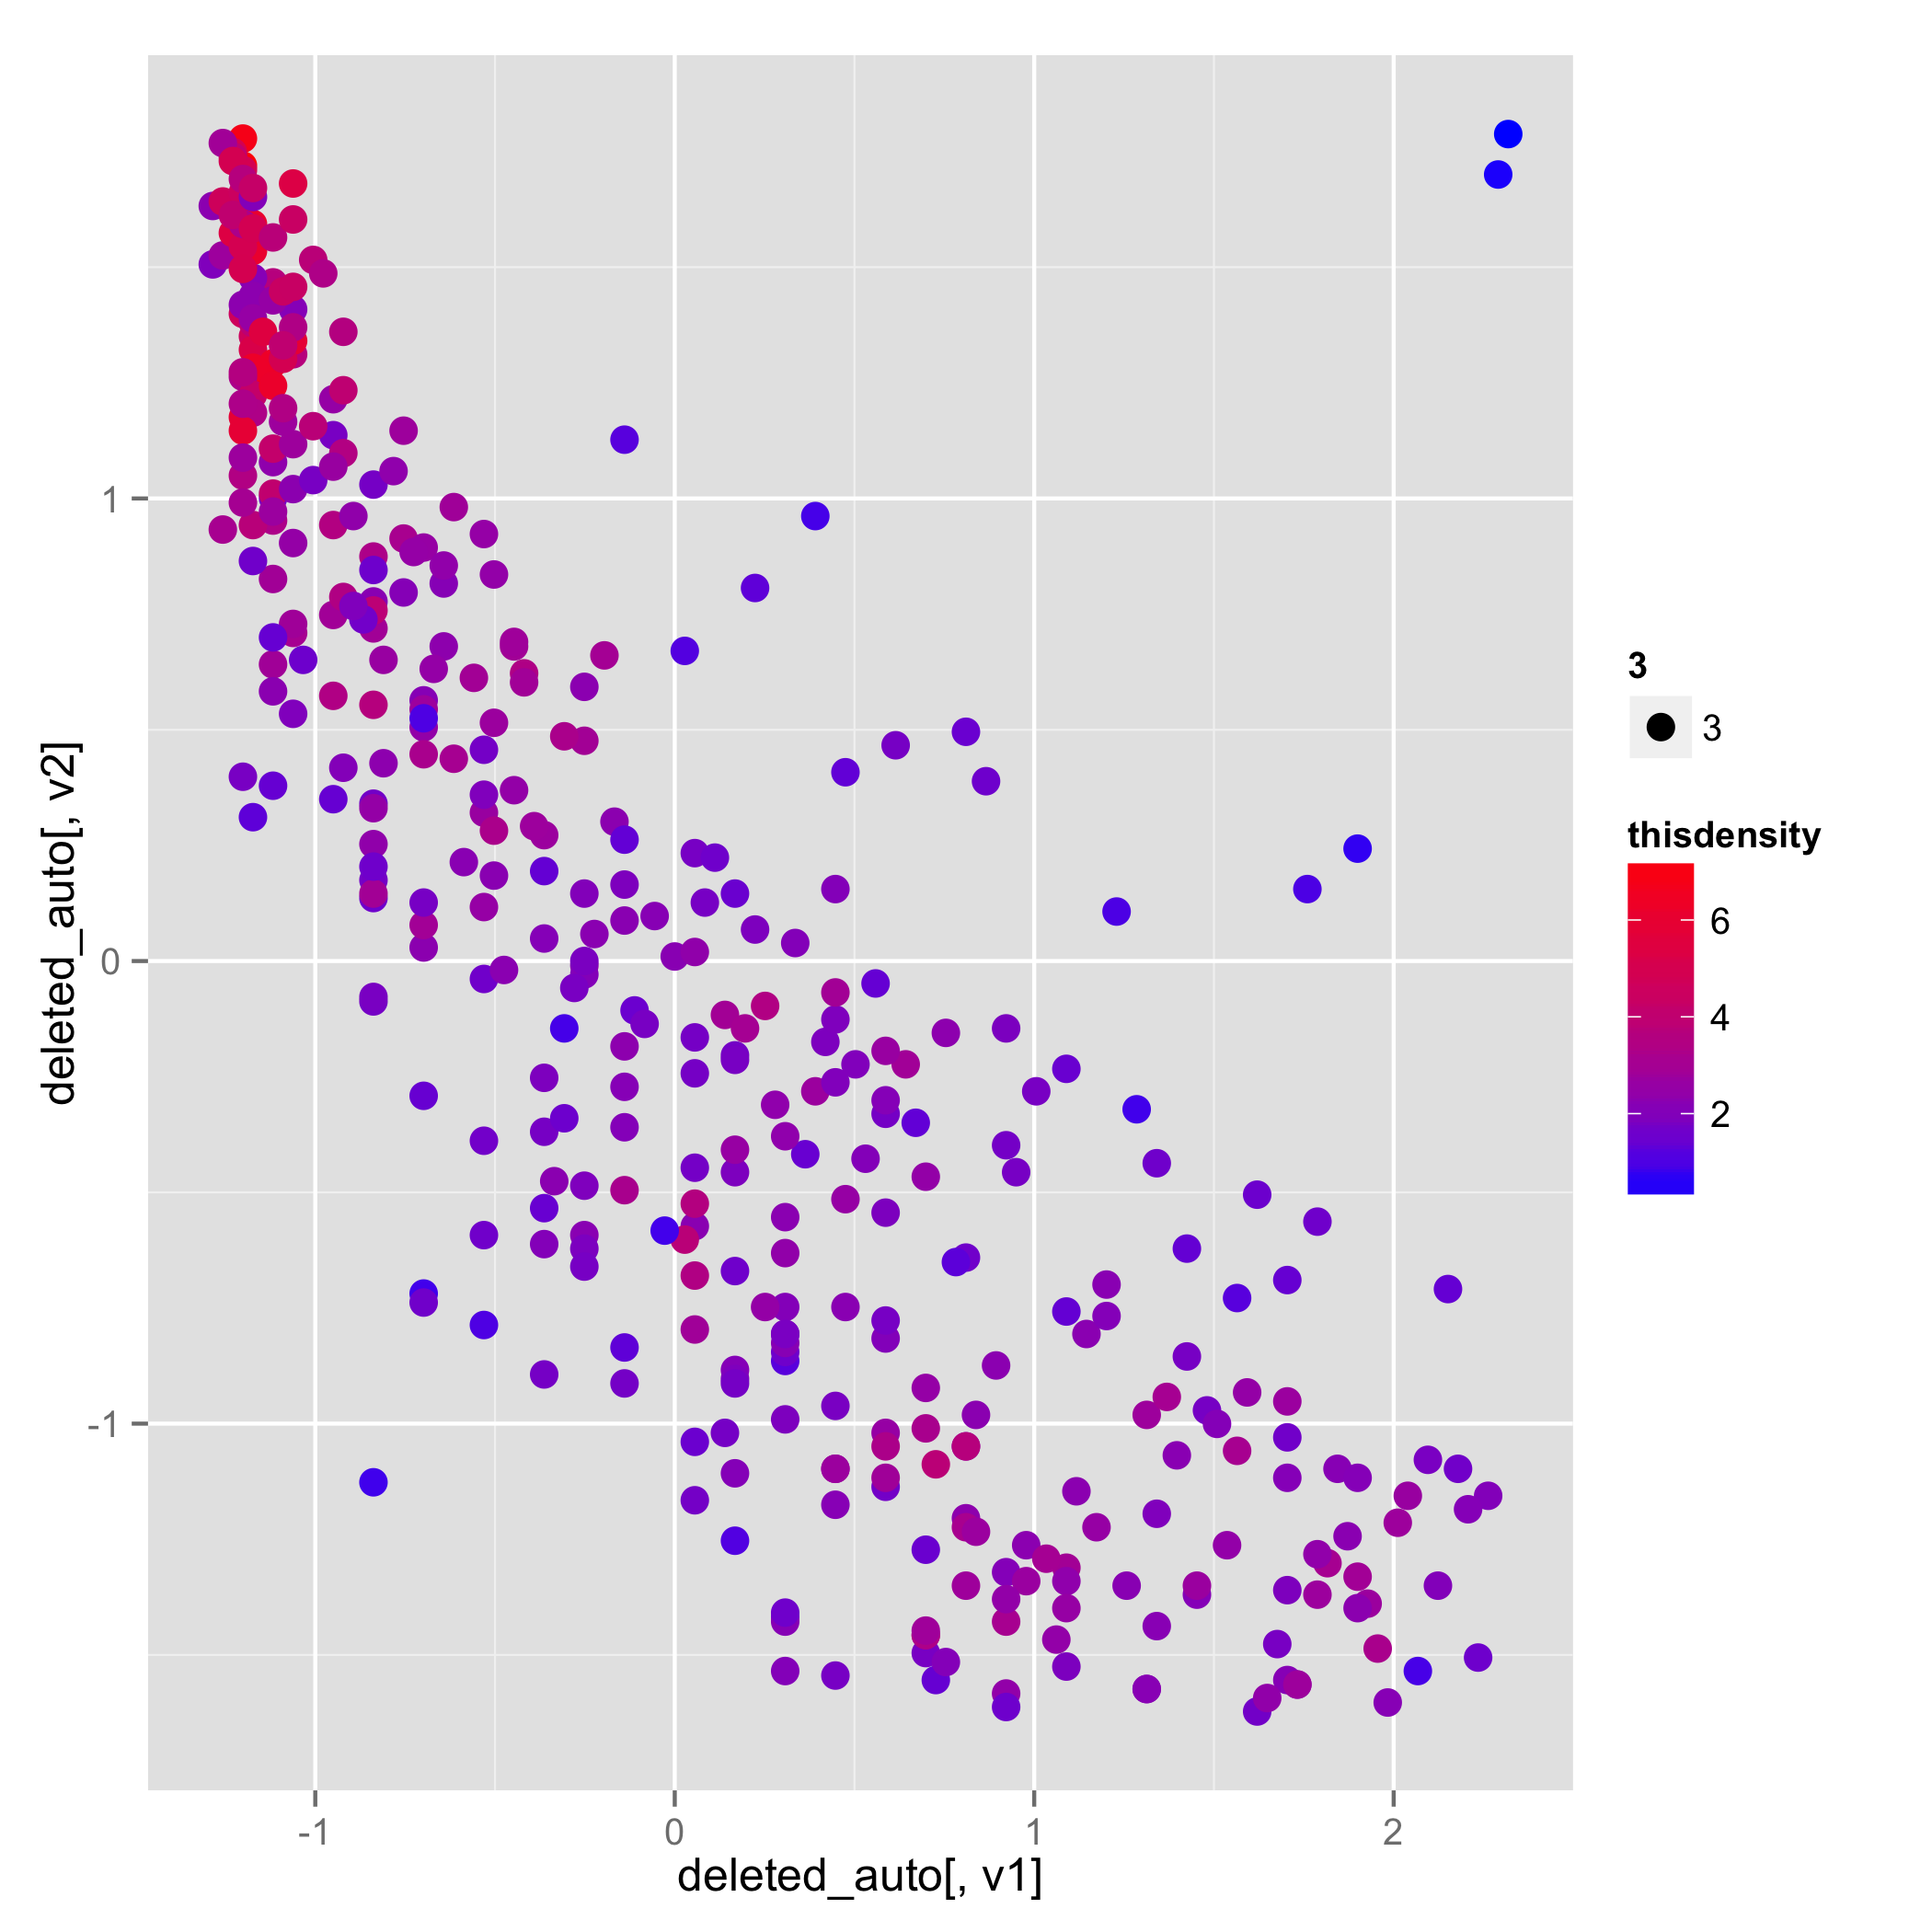
\includegraphics[scale=0.05]{using_density1_5.png}
\par\end{centering}}
\quad{}
\subfloat[]{\begin{centering}
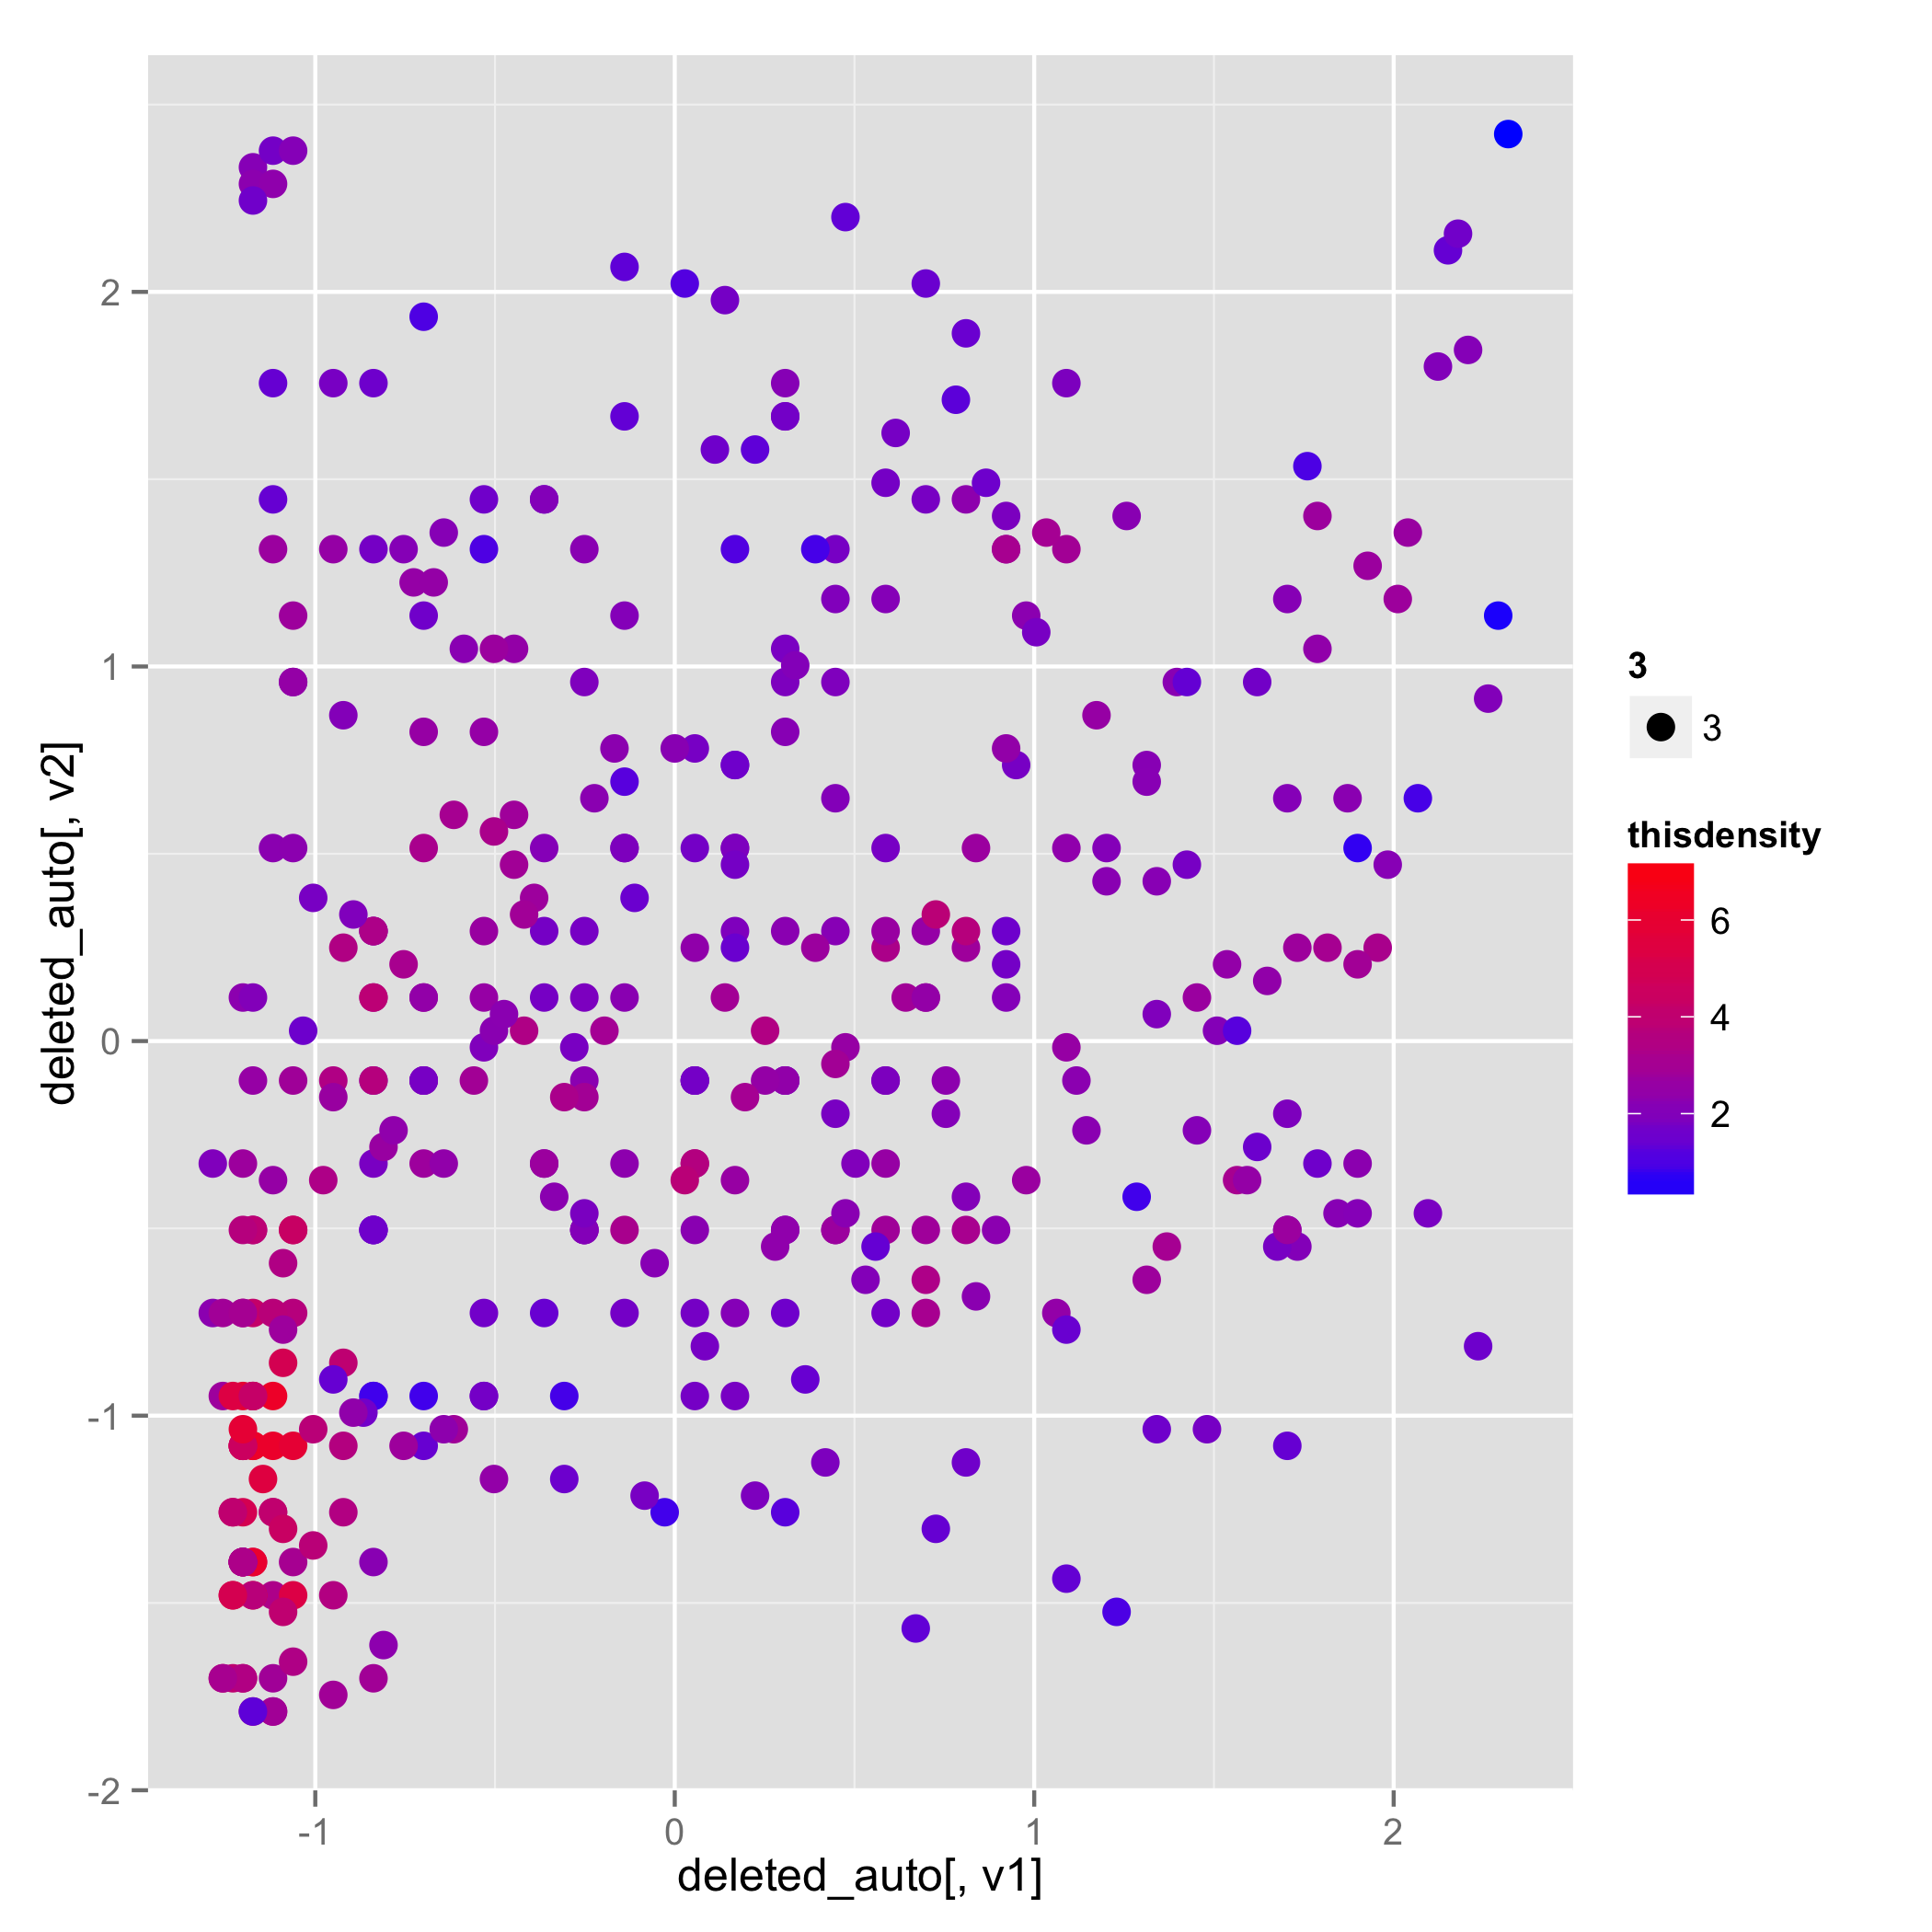
\includegraphics[scale=0.05]{using_density1_6.png}
\par\end{centering}}
\quad{}
\subfloat[]{\begin{centering}
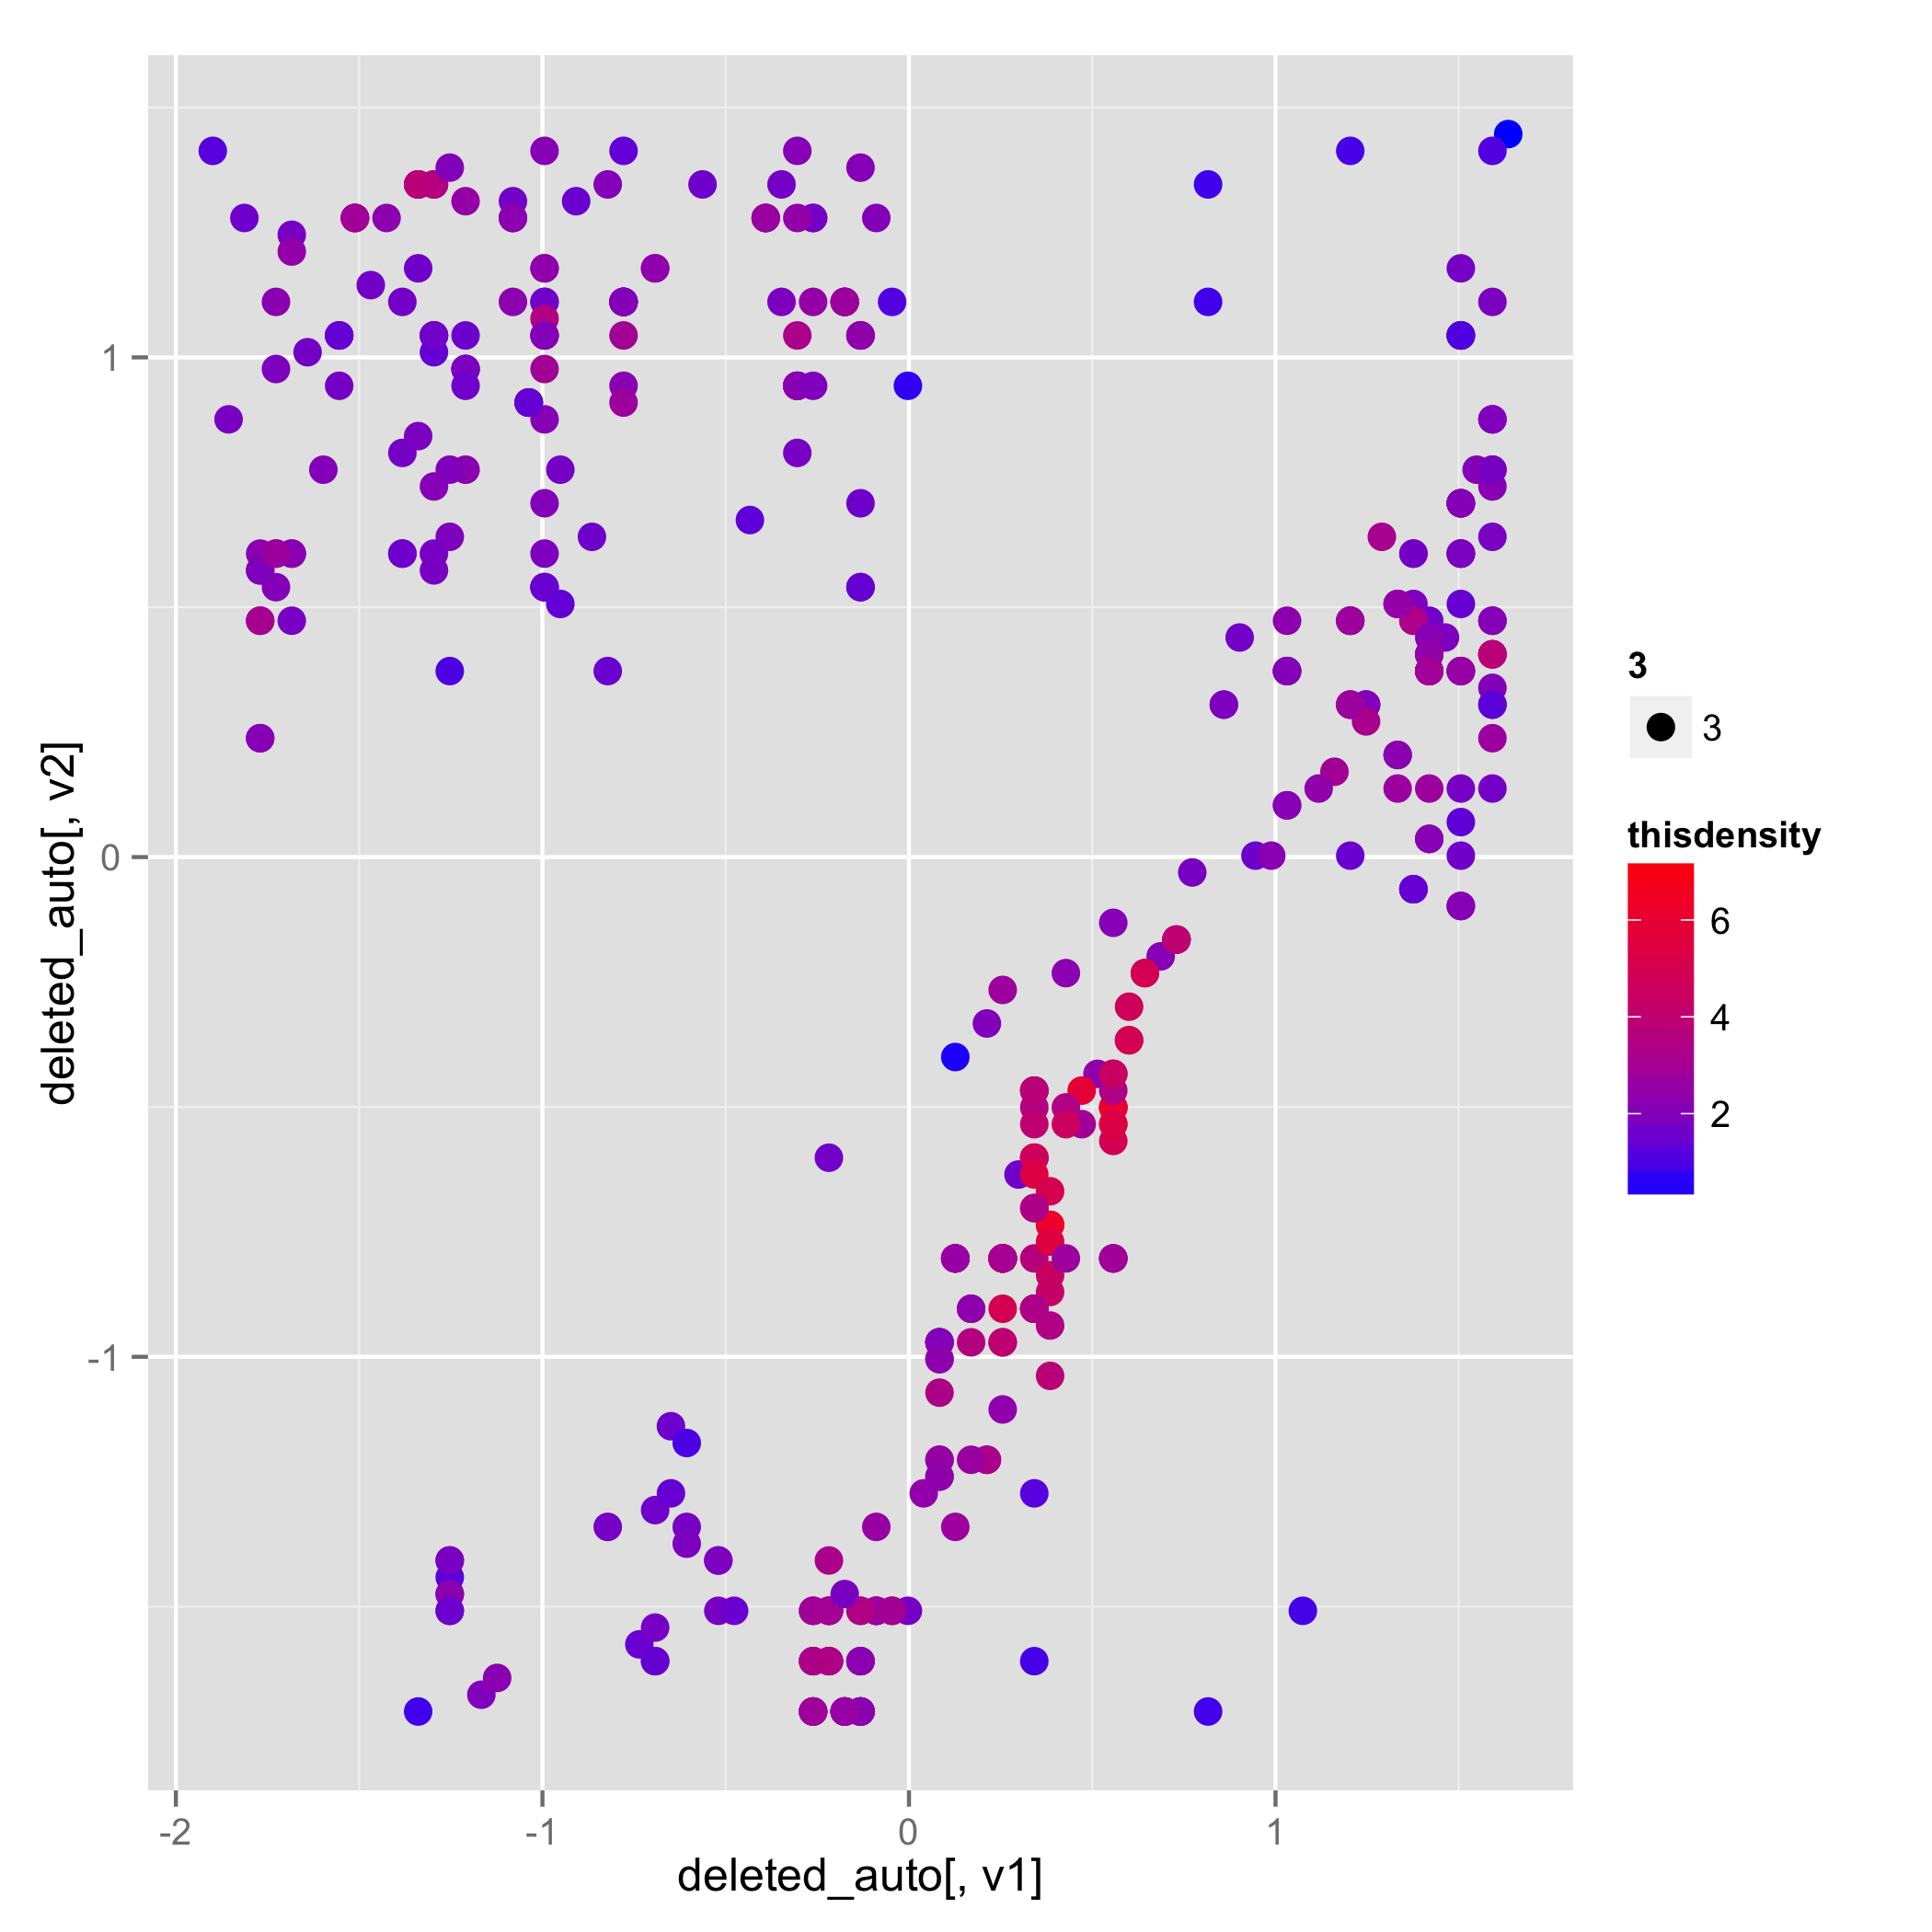
\includegraphics[scale=0.05]{using_density3_4.png}
\par\end{centering}}
\quad{}
\subfloat[]{\begin{centering}
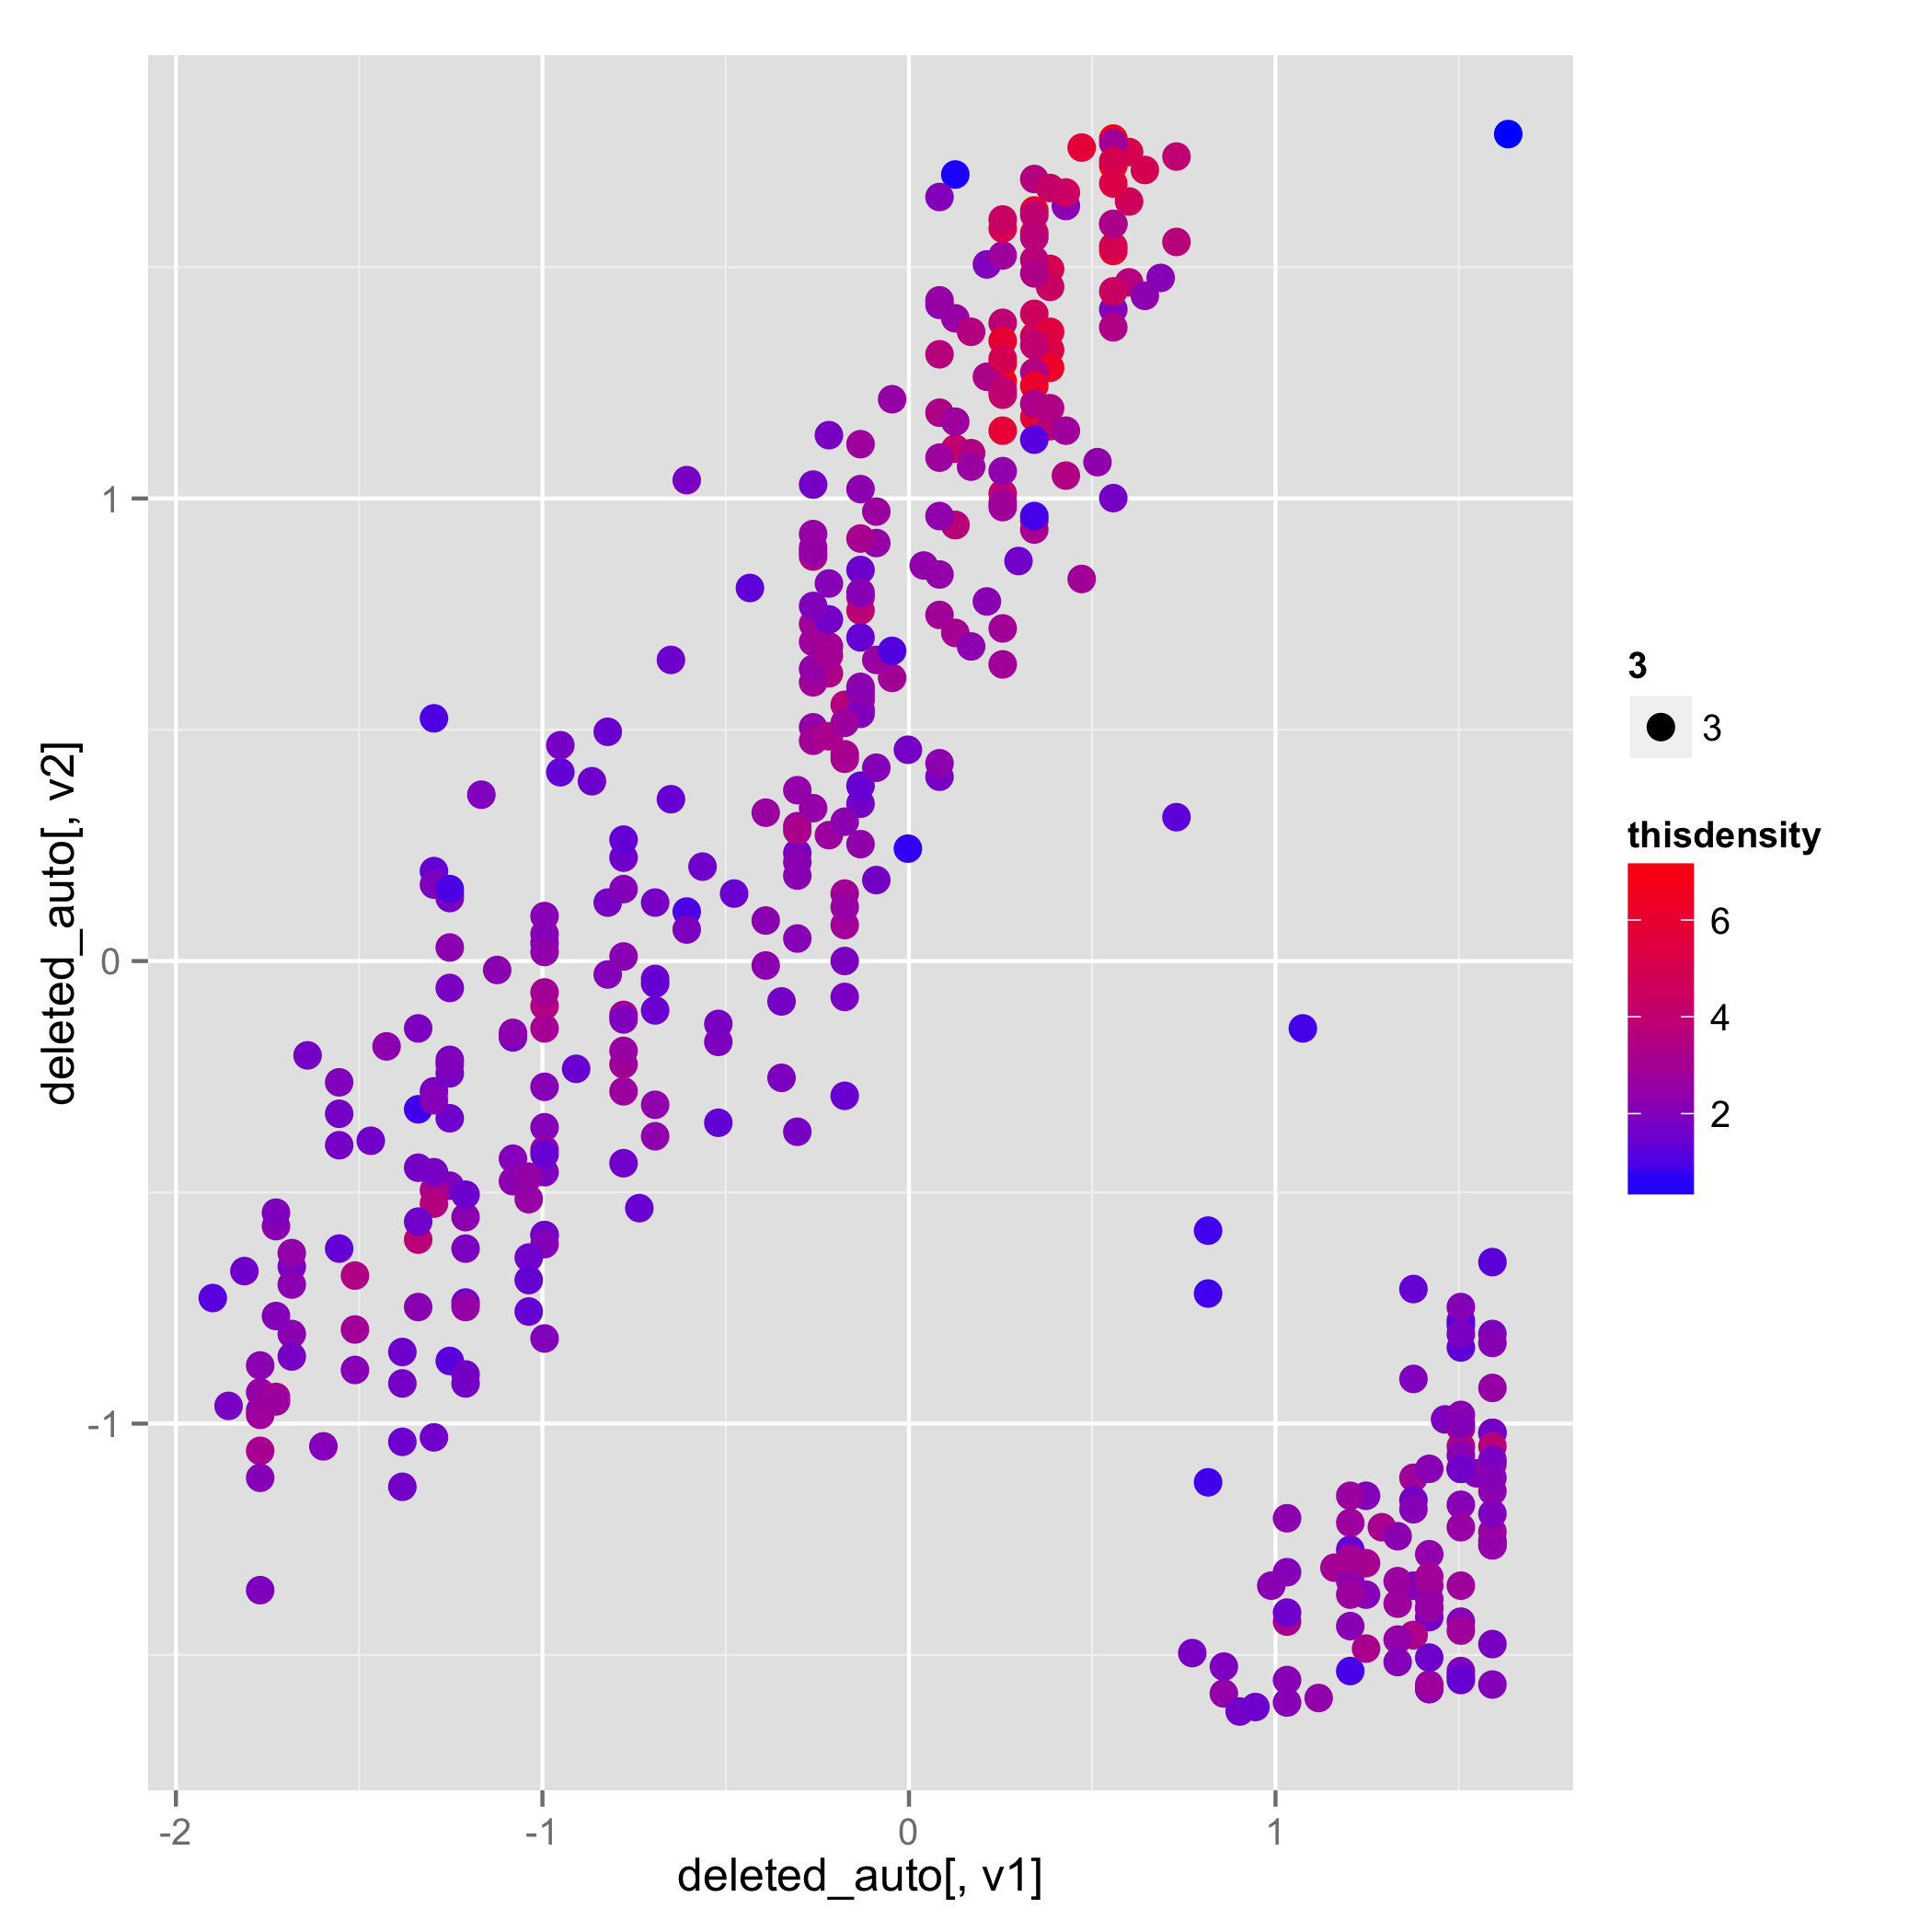
\includegraphics[scale=0.05]{using_density3_5.png}
\par\end{centering}}
\quad{}
\subfloat[]{\begin{centering}
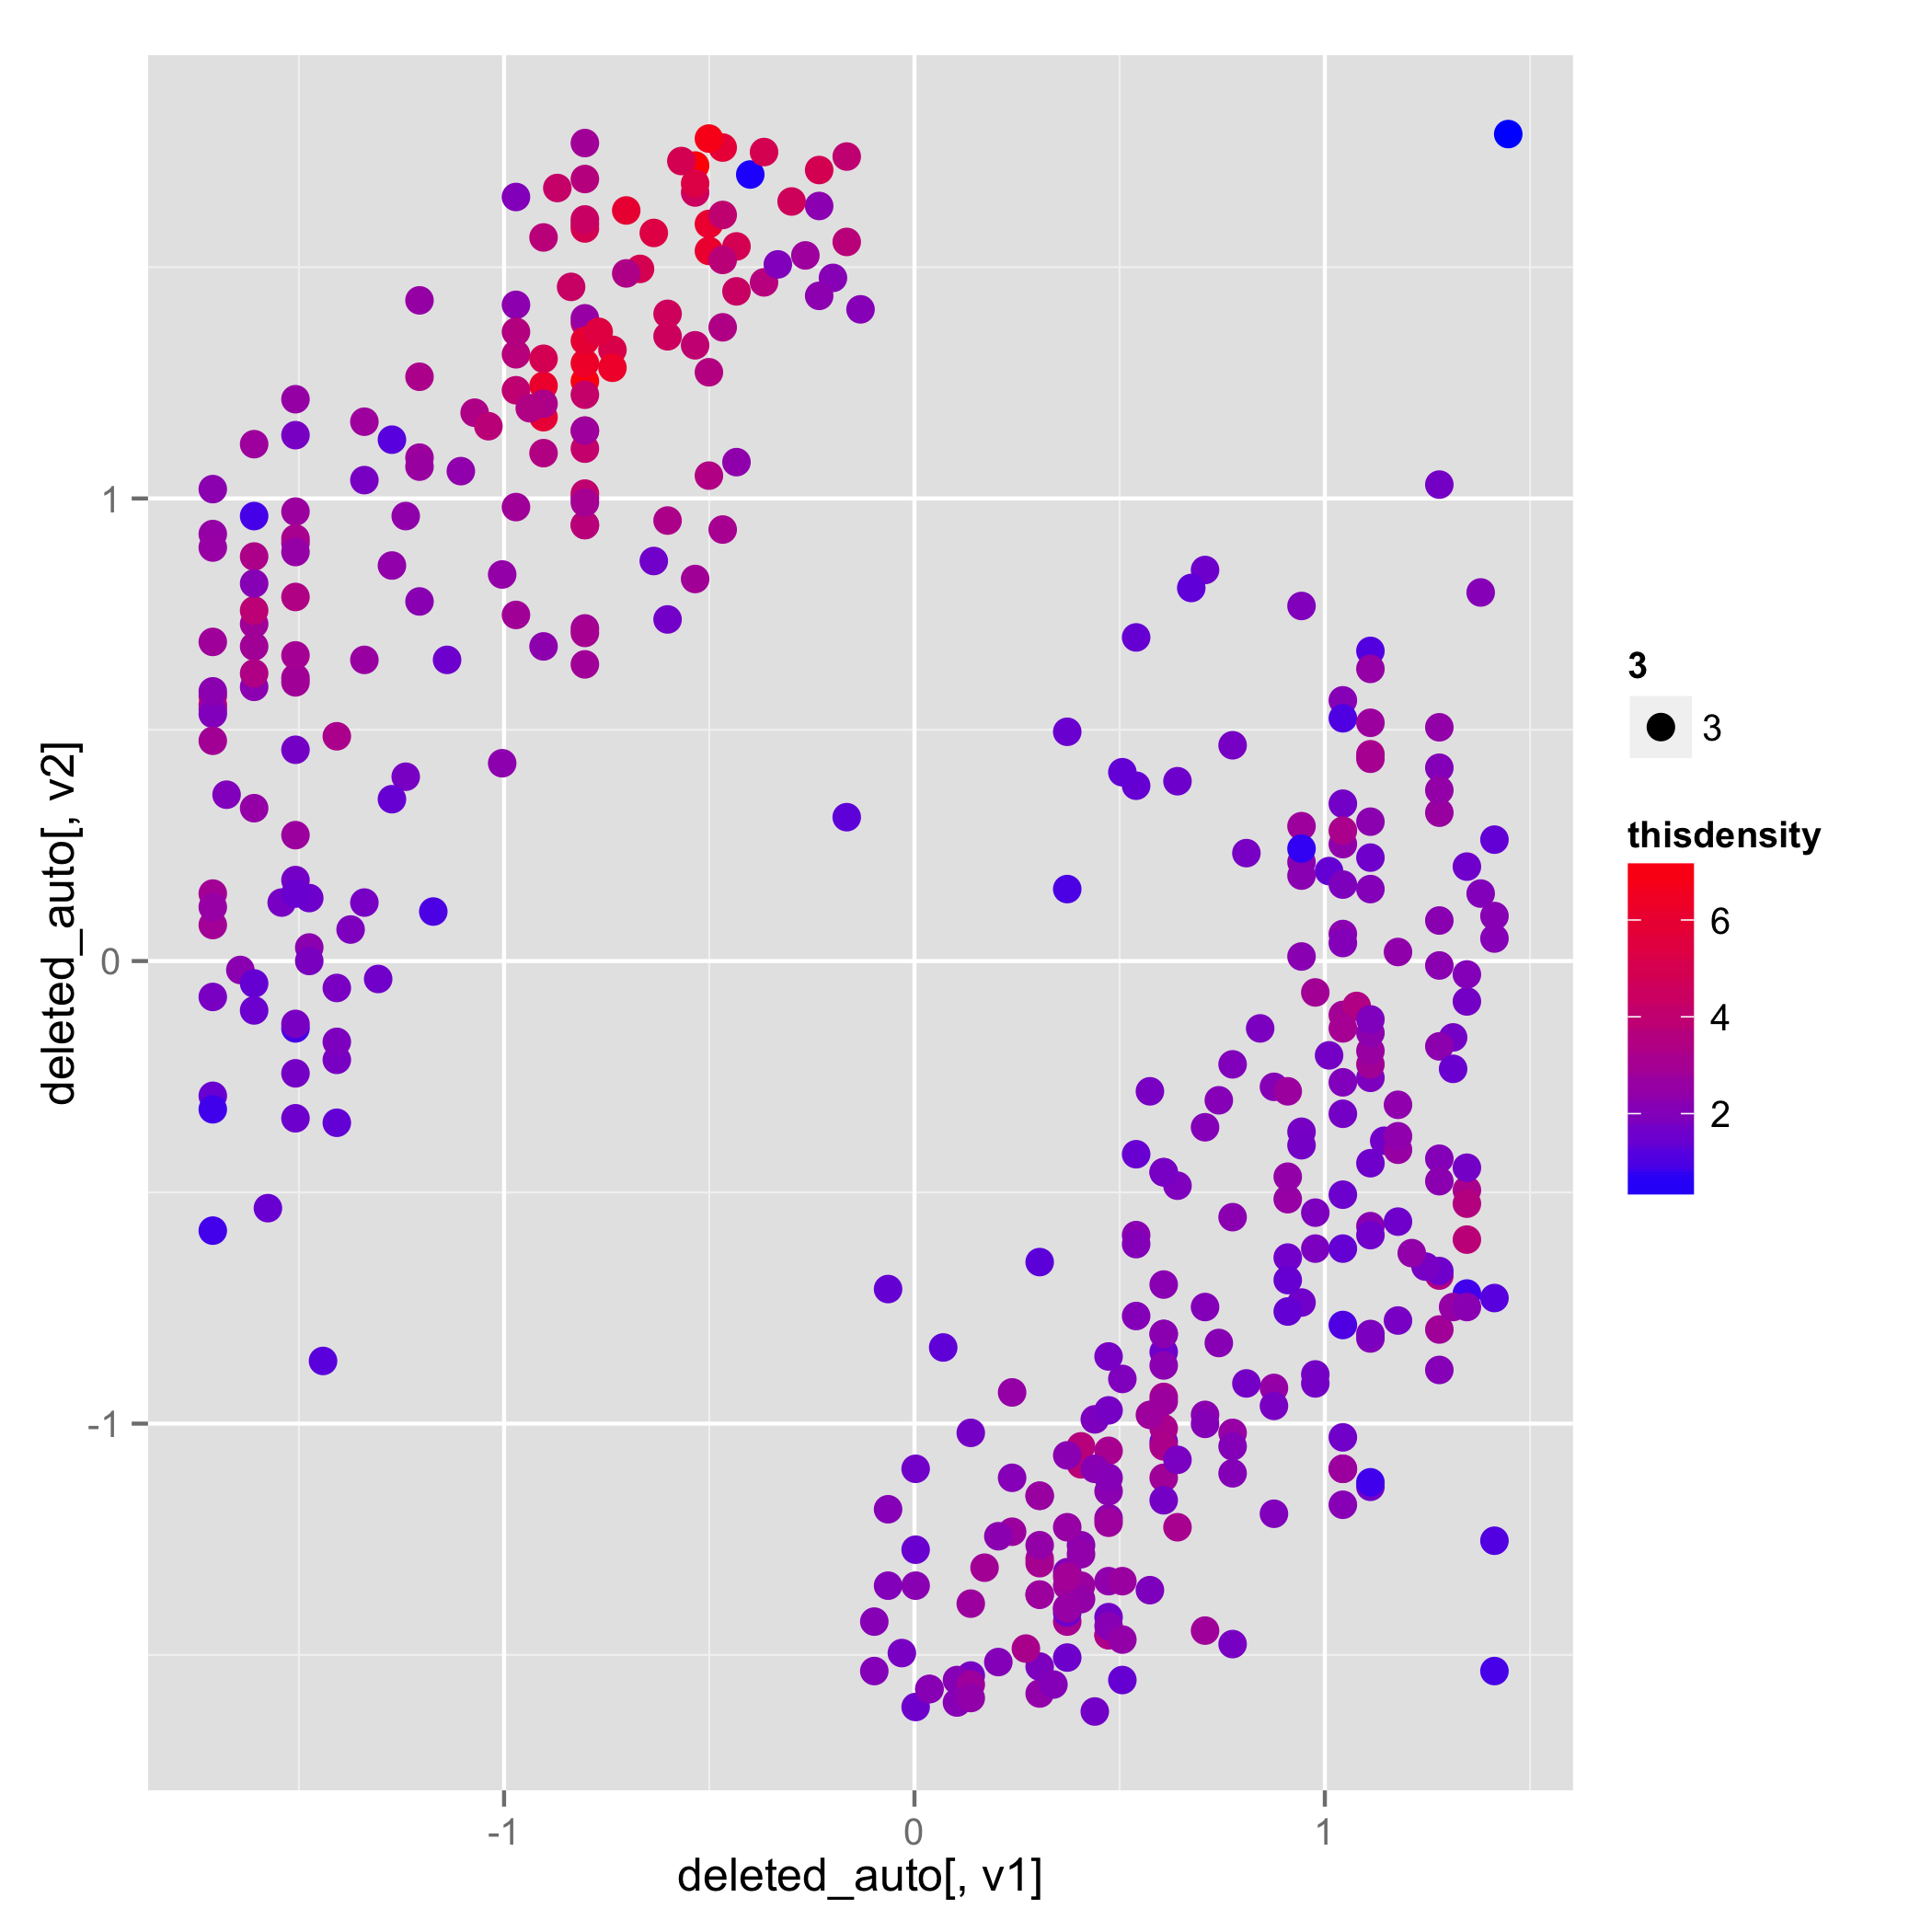
\includegraphics[scale=0.05]{using_density4_5.png}
\par\end{centering}}
\quad{}
\subfloat[]{\begin{centering}
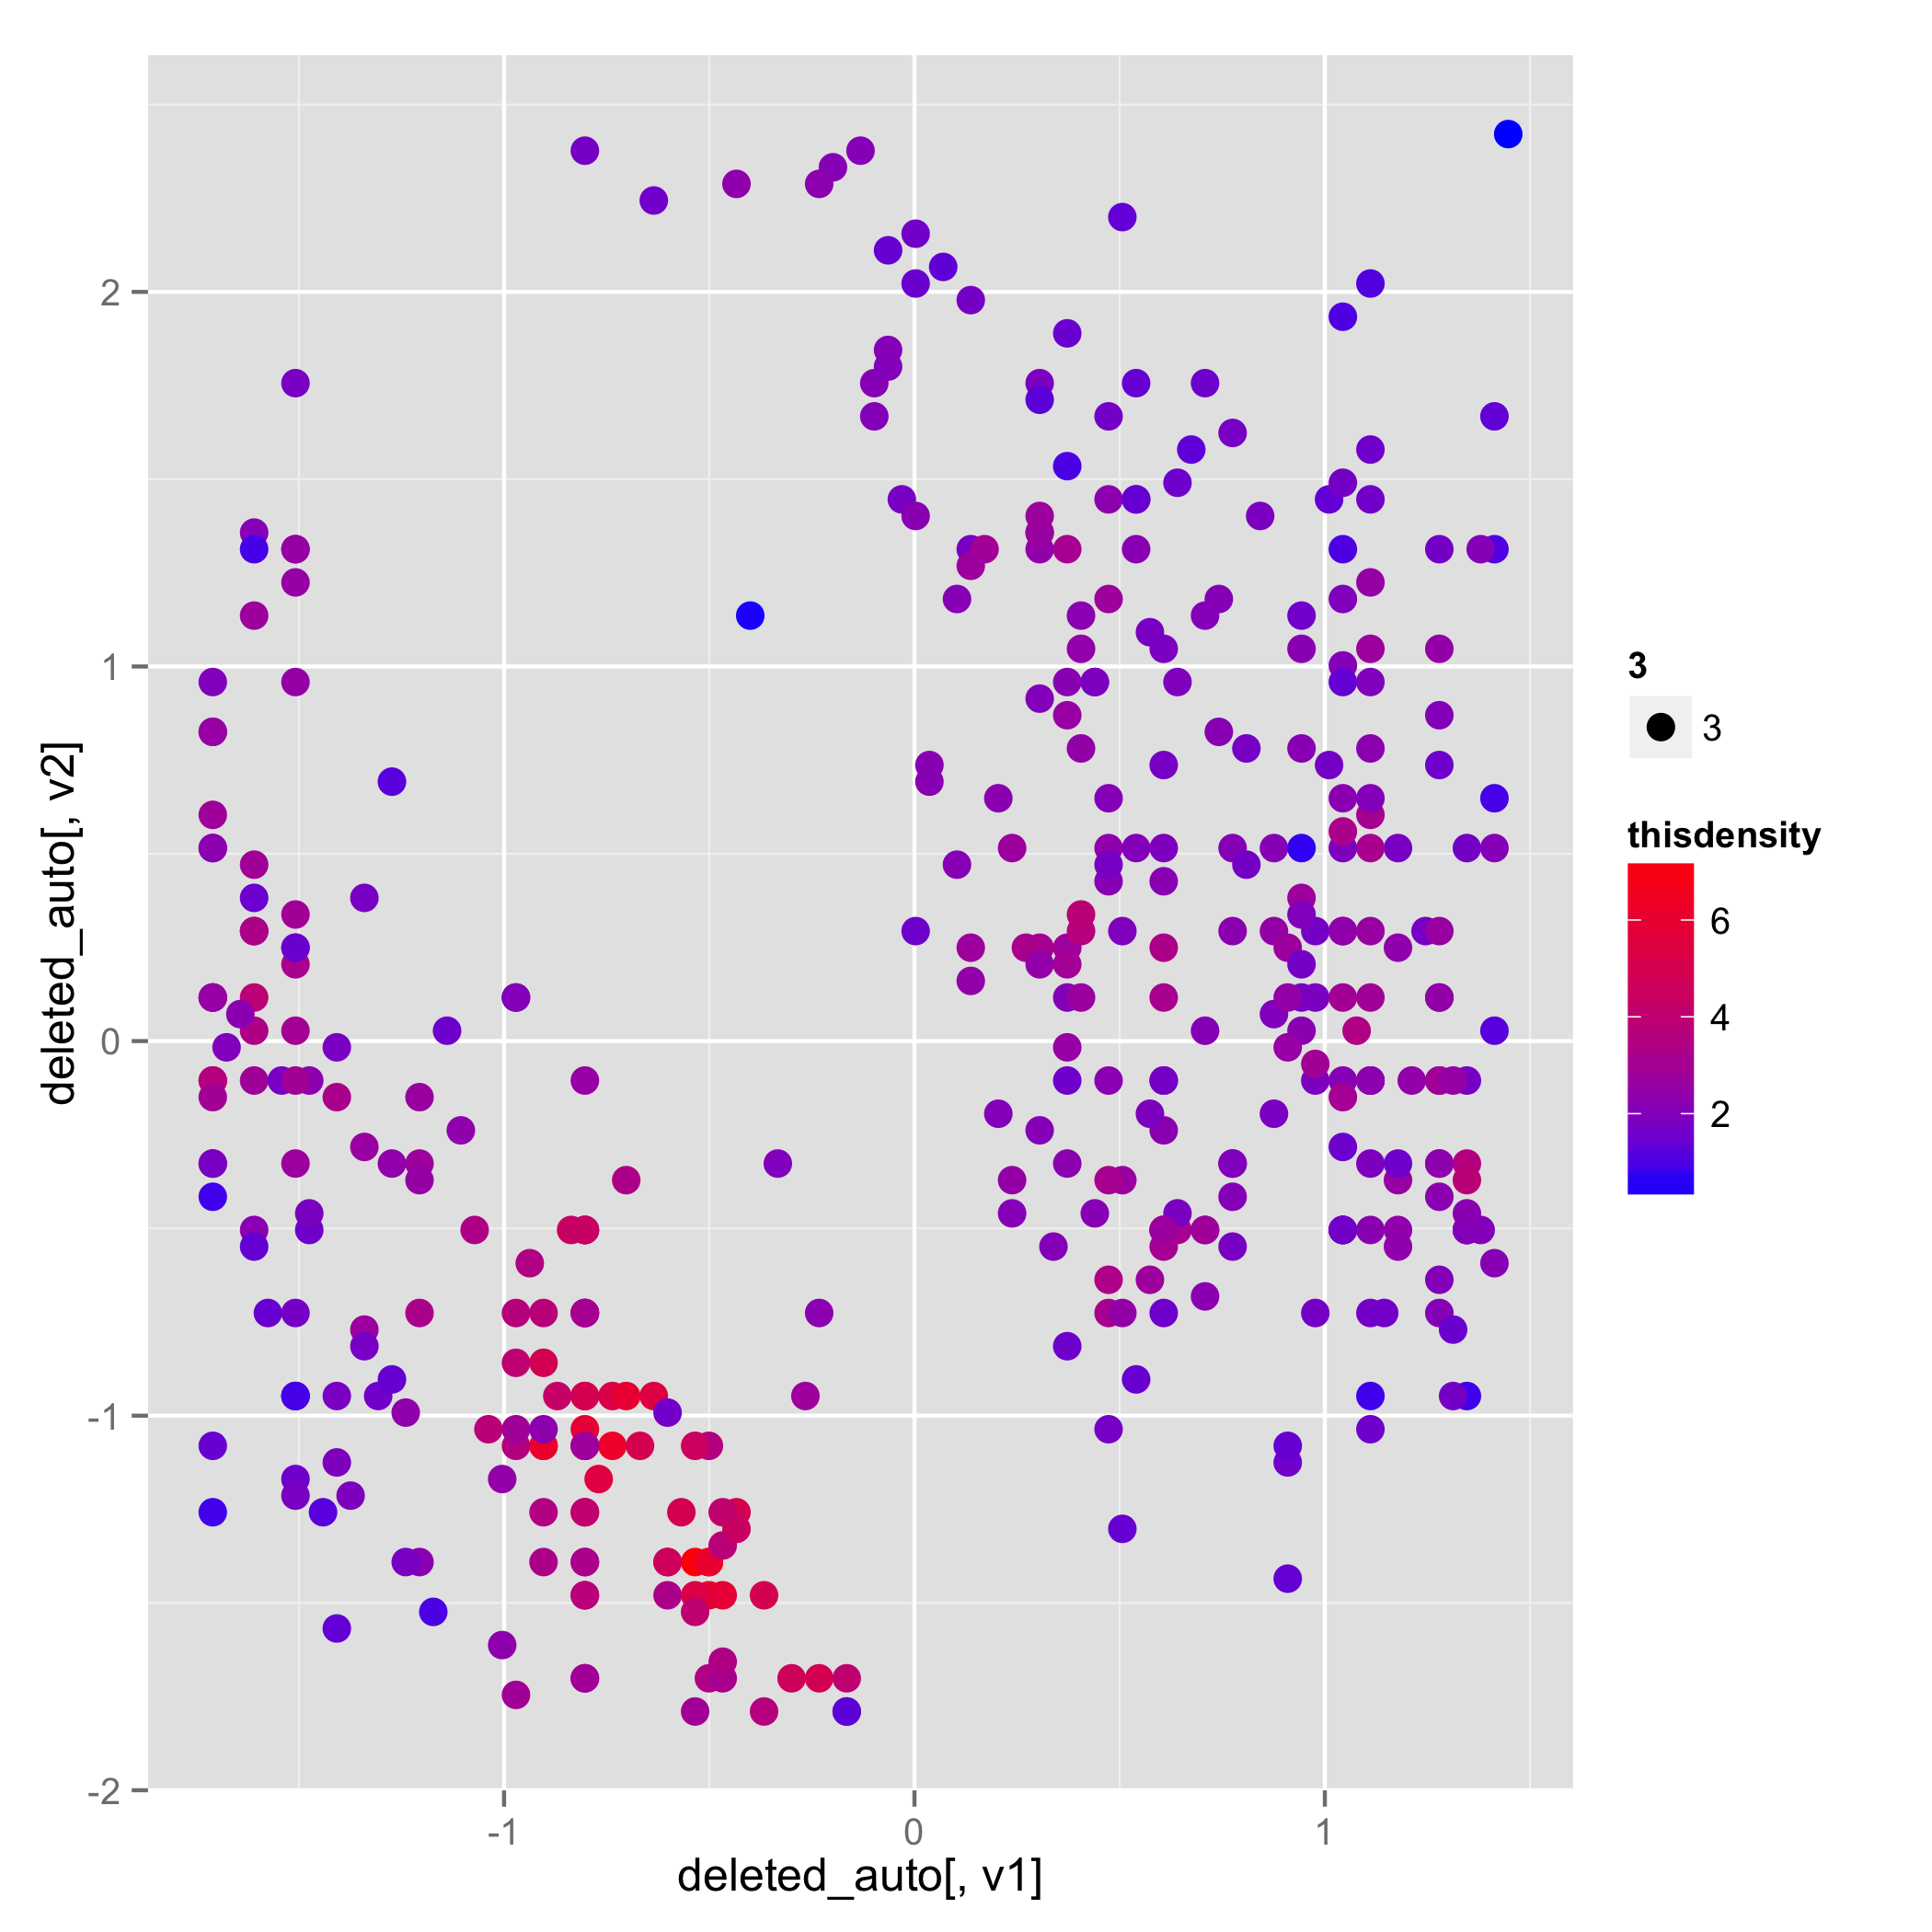
\includegraphics[scale=0.05]{using_density4_6.png}
\par\end{centering}}
\quad{}
\subfloat[]{\begin{centering}
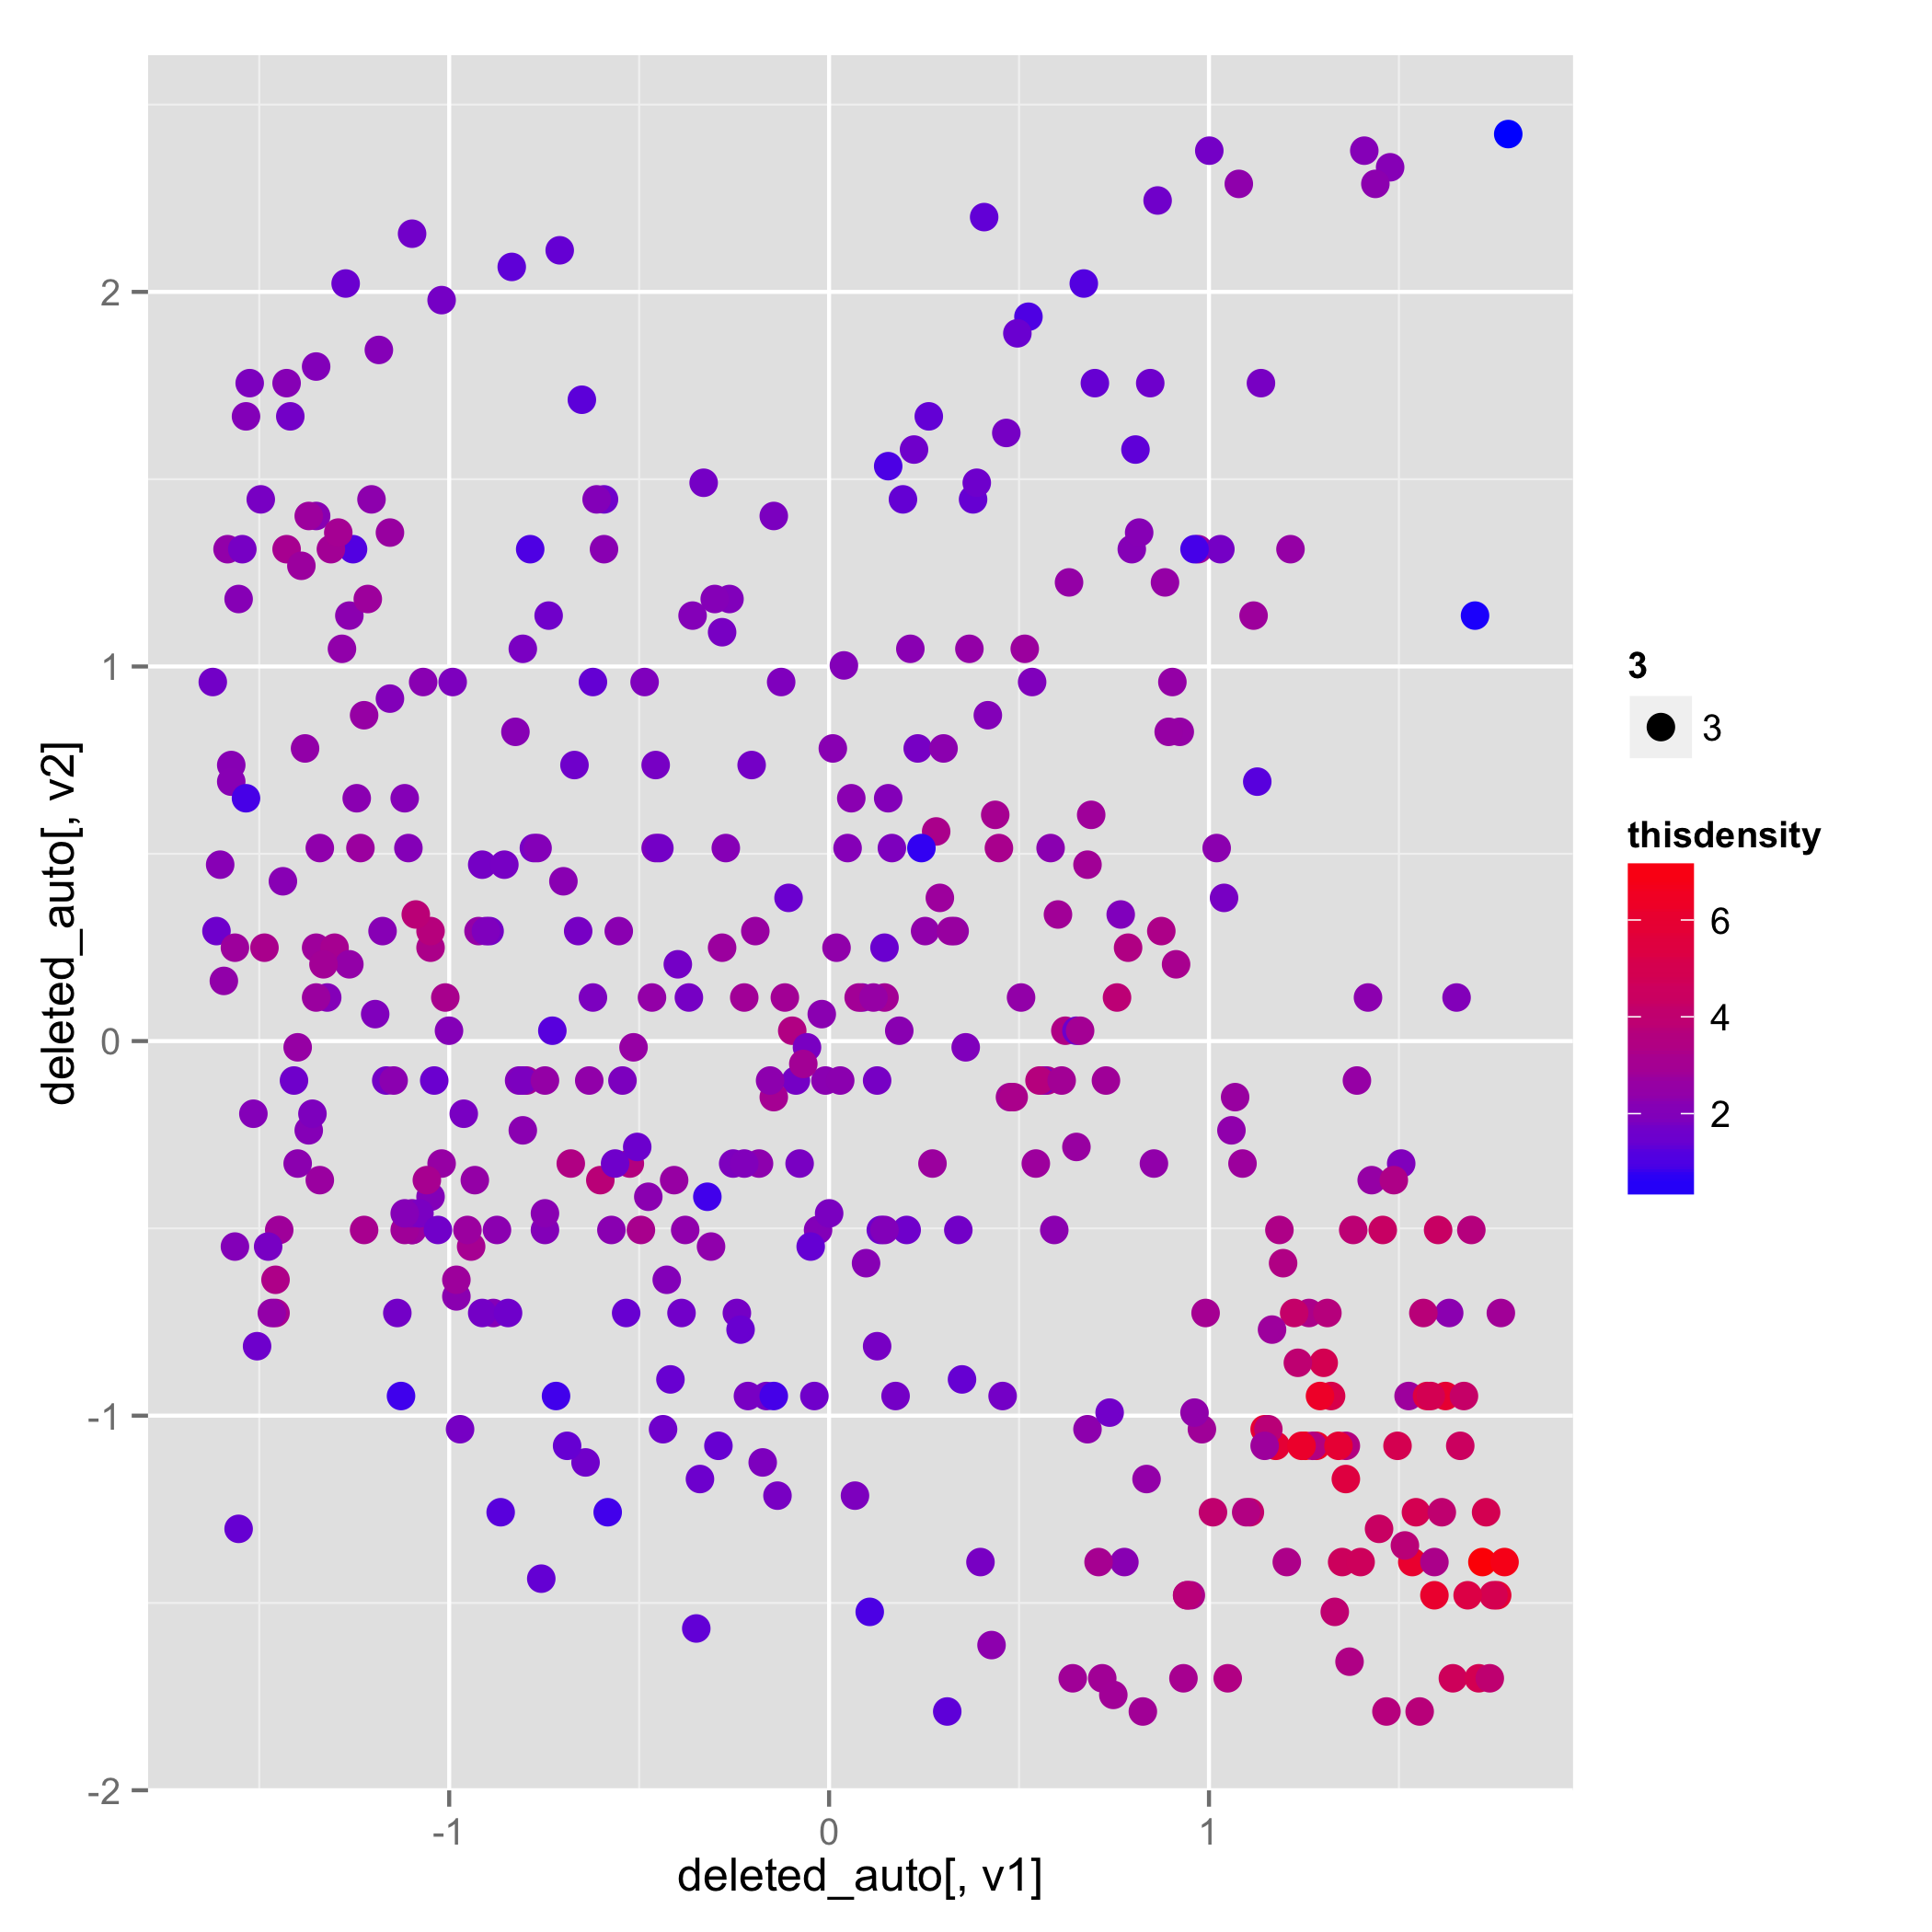
\includegraphics[scale=0.05]{using_density5_6.png}
\par\end{centering}}
\end{center}
\end{figure}


\item Using local outlier factor as a metric, there are 3 likely cutoff points. 
The three considered here are values of 1.8, 2.0, and 2.5. 
For the ggplot visualization, the cutoff was set at 2.0.


\begin{center}
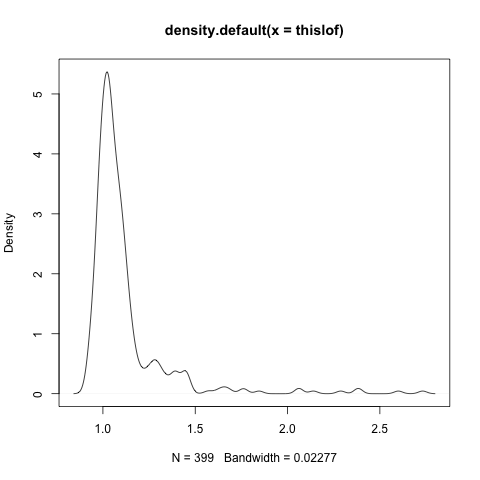
\includegraphics[scale=0.35]{density_lof}
\end{center}

    %# local outlier factor:
%    thislof = lofactor(deleted_auto[,cols],k = 5)
%    plot(density(thislof))
%
%    (1:nrow(deleted_auto))[thislof >= 1.25]
%   1  15  27  28  29  30  34  51  56  61  73  87  93 105 110 113 121 141 
%  142 144 146 149 156 157 167 168 189 205 211 213 215 217 231 245 265 279 
%  288 294 300 327 328 329 332 335 336 354 356 359 366 376 388 389 391 396
%    (1:nrow(deleted_auto))[thislof >= 1.5]
%   1  15  27  30  73 113 205 245 265 300 332 336 359 366 388 389


\begin{figure}[H]
\begin{center}
\subfloat[]{\begin{centering}
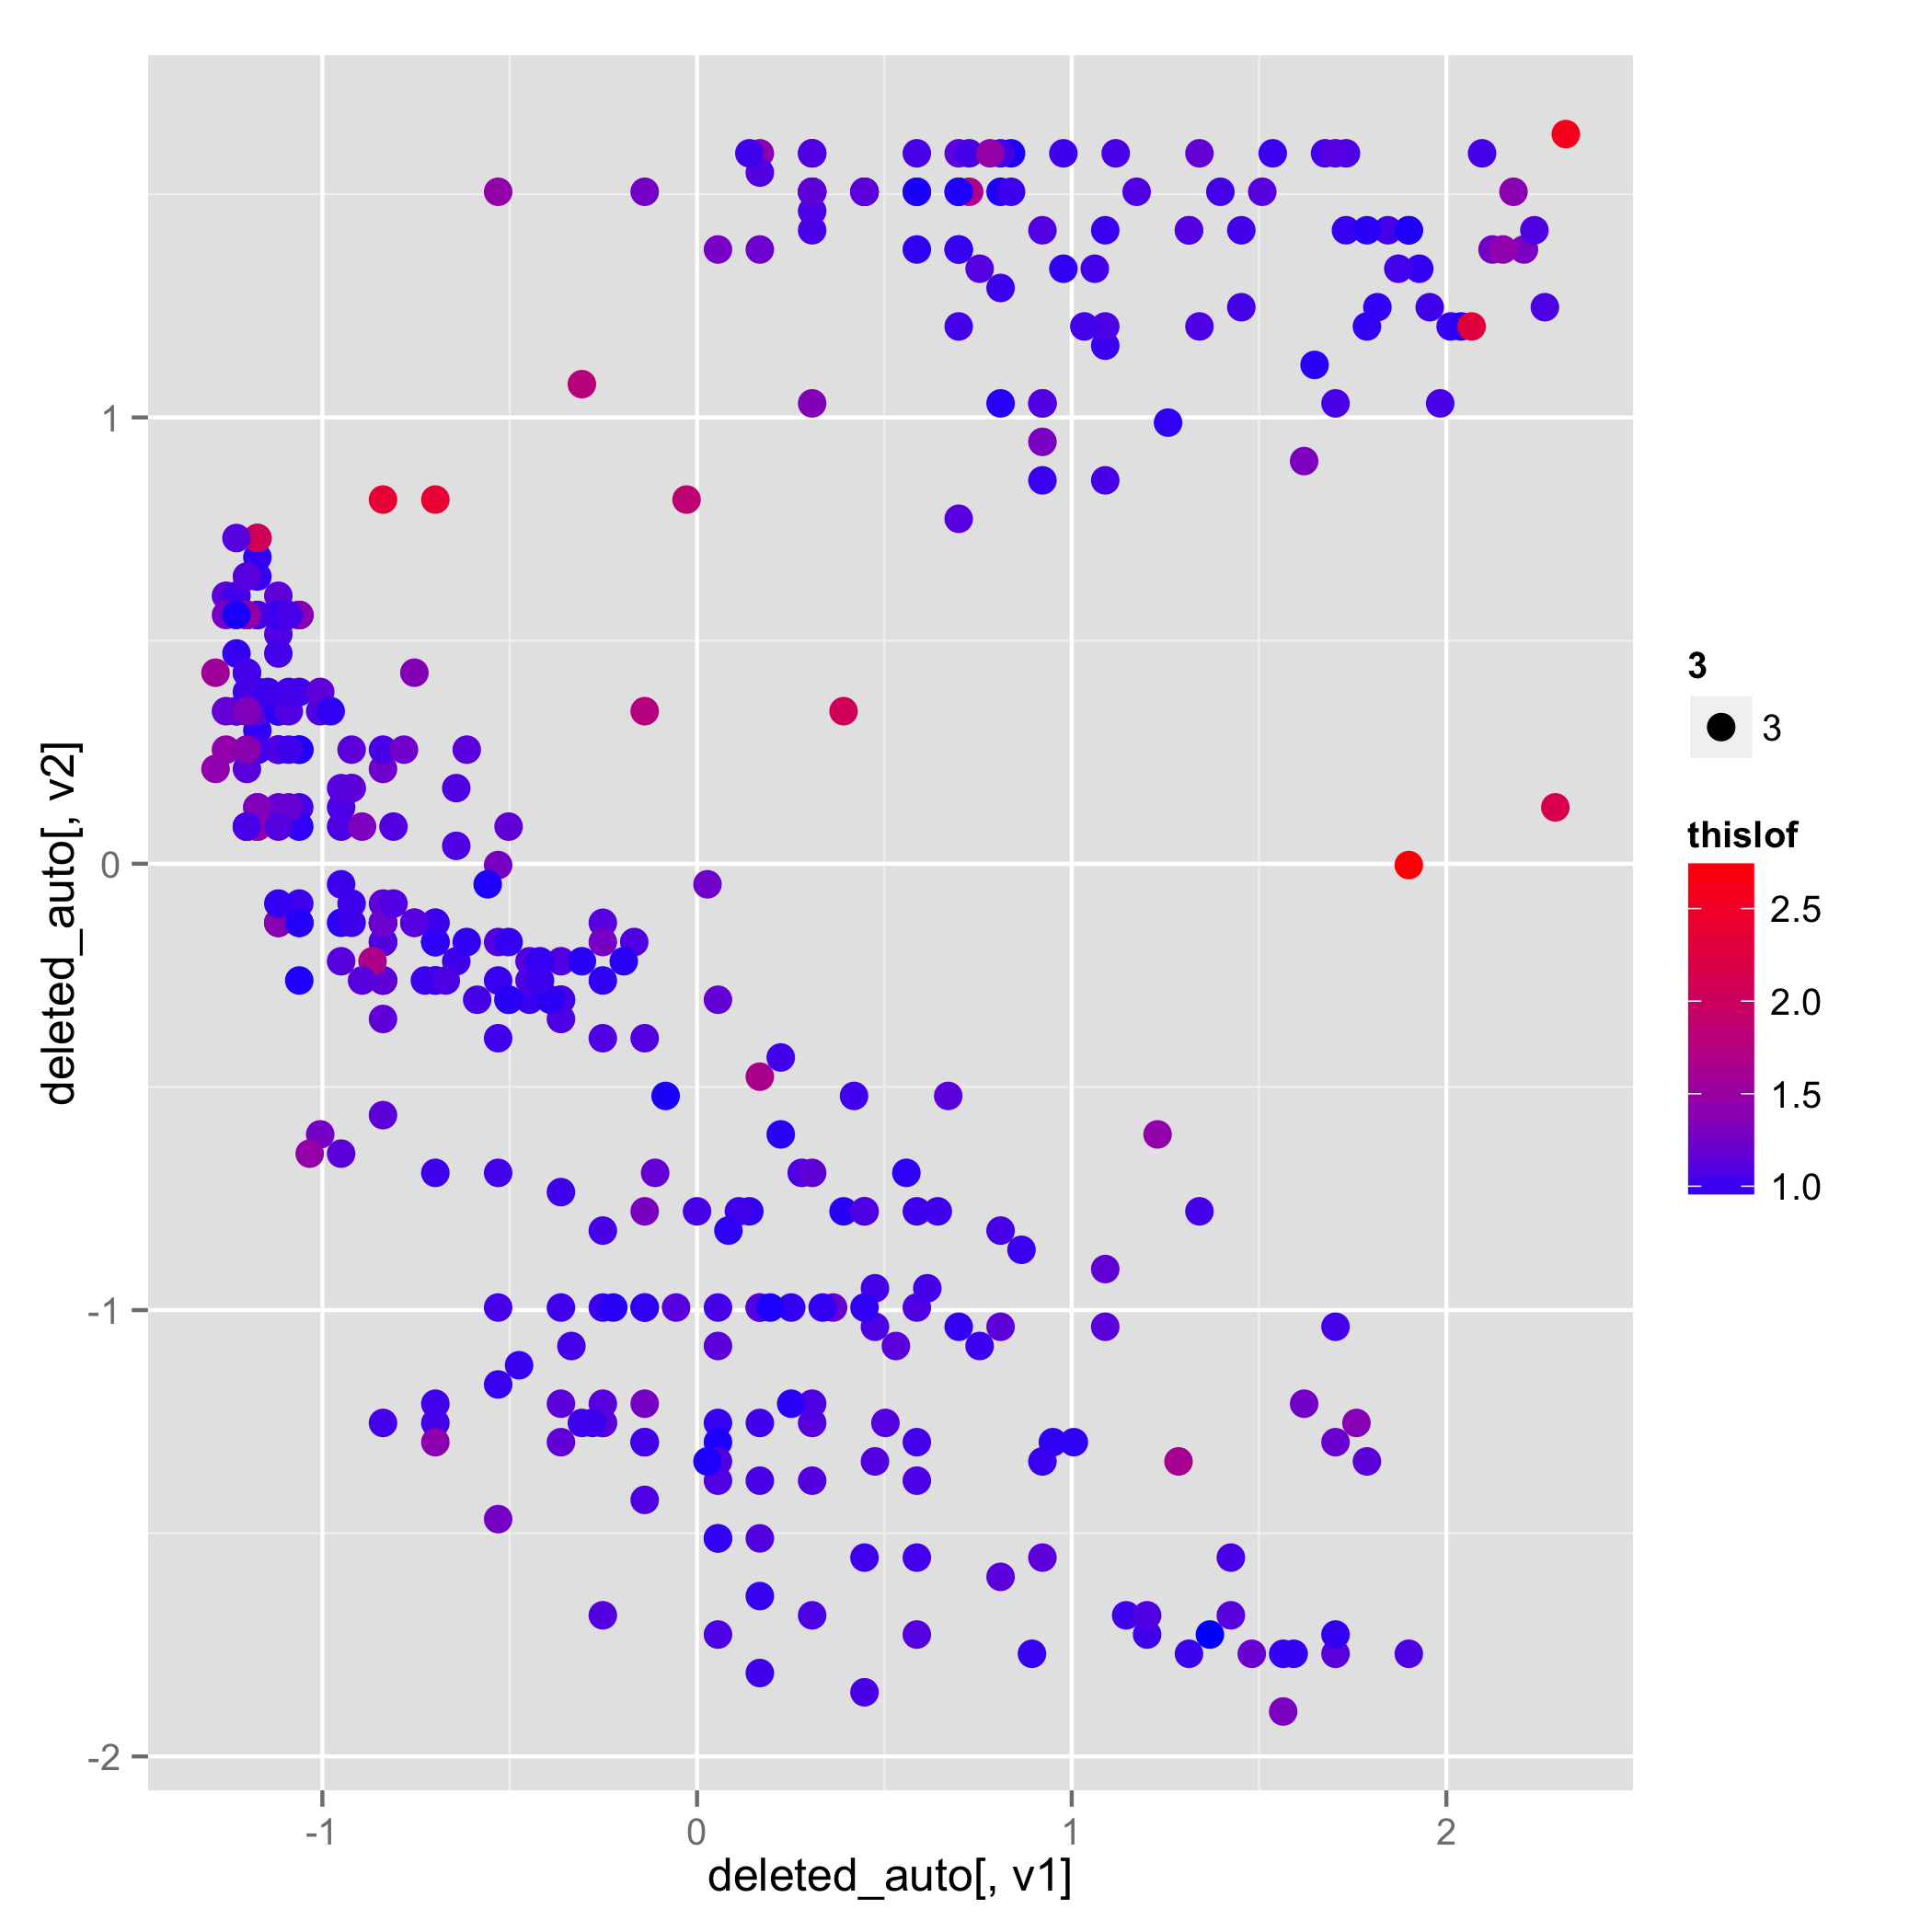
\includegraphics[scale=0.05]{using_lof1_3.png}
\par\end{centering}}
\quad{}
\subfloat[]{\begin{centering}
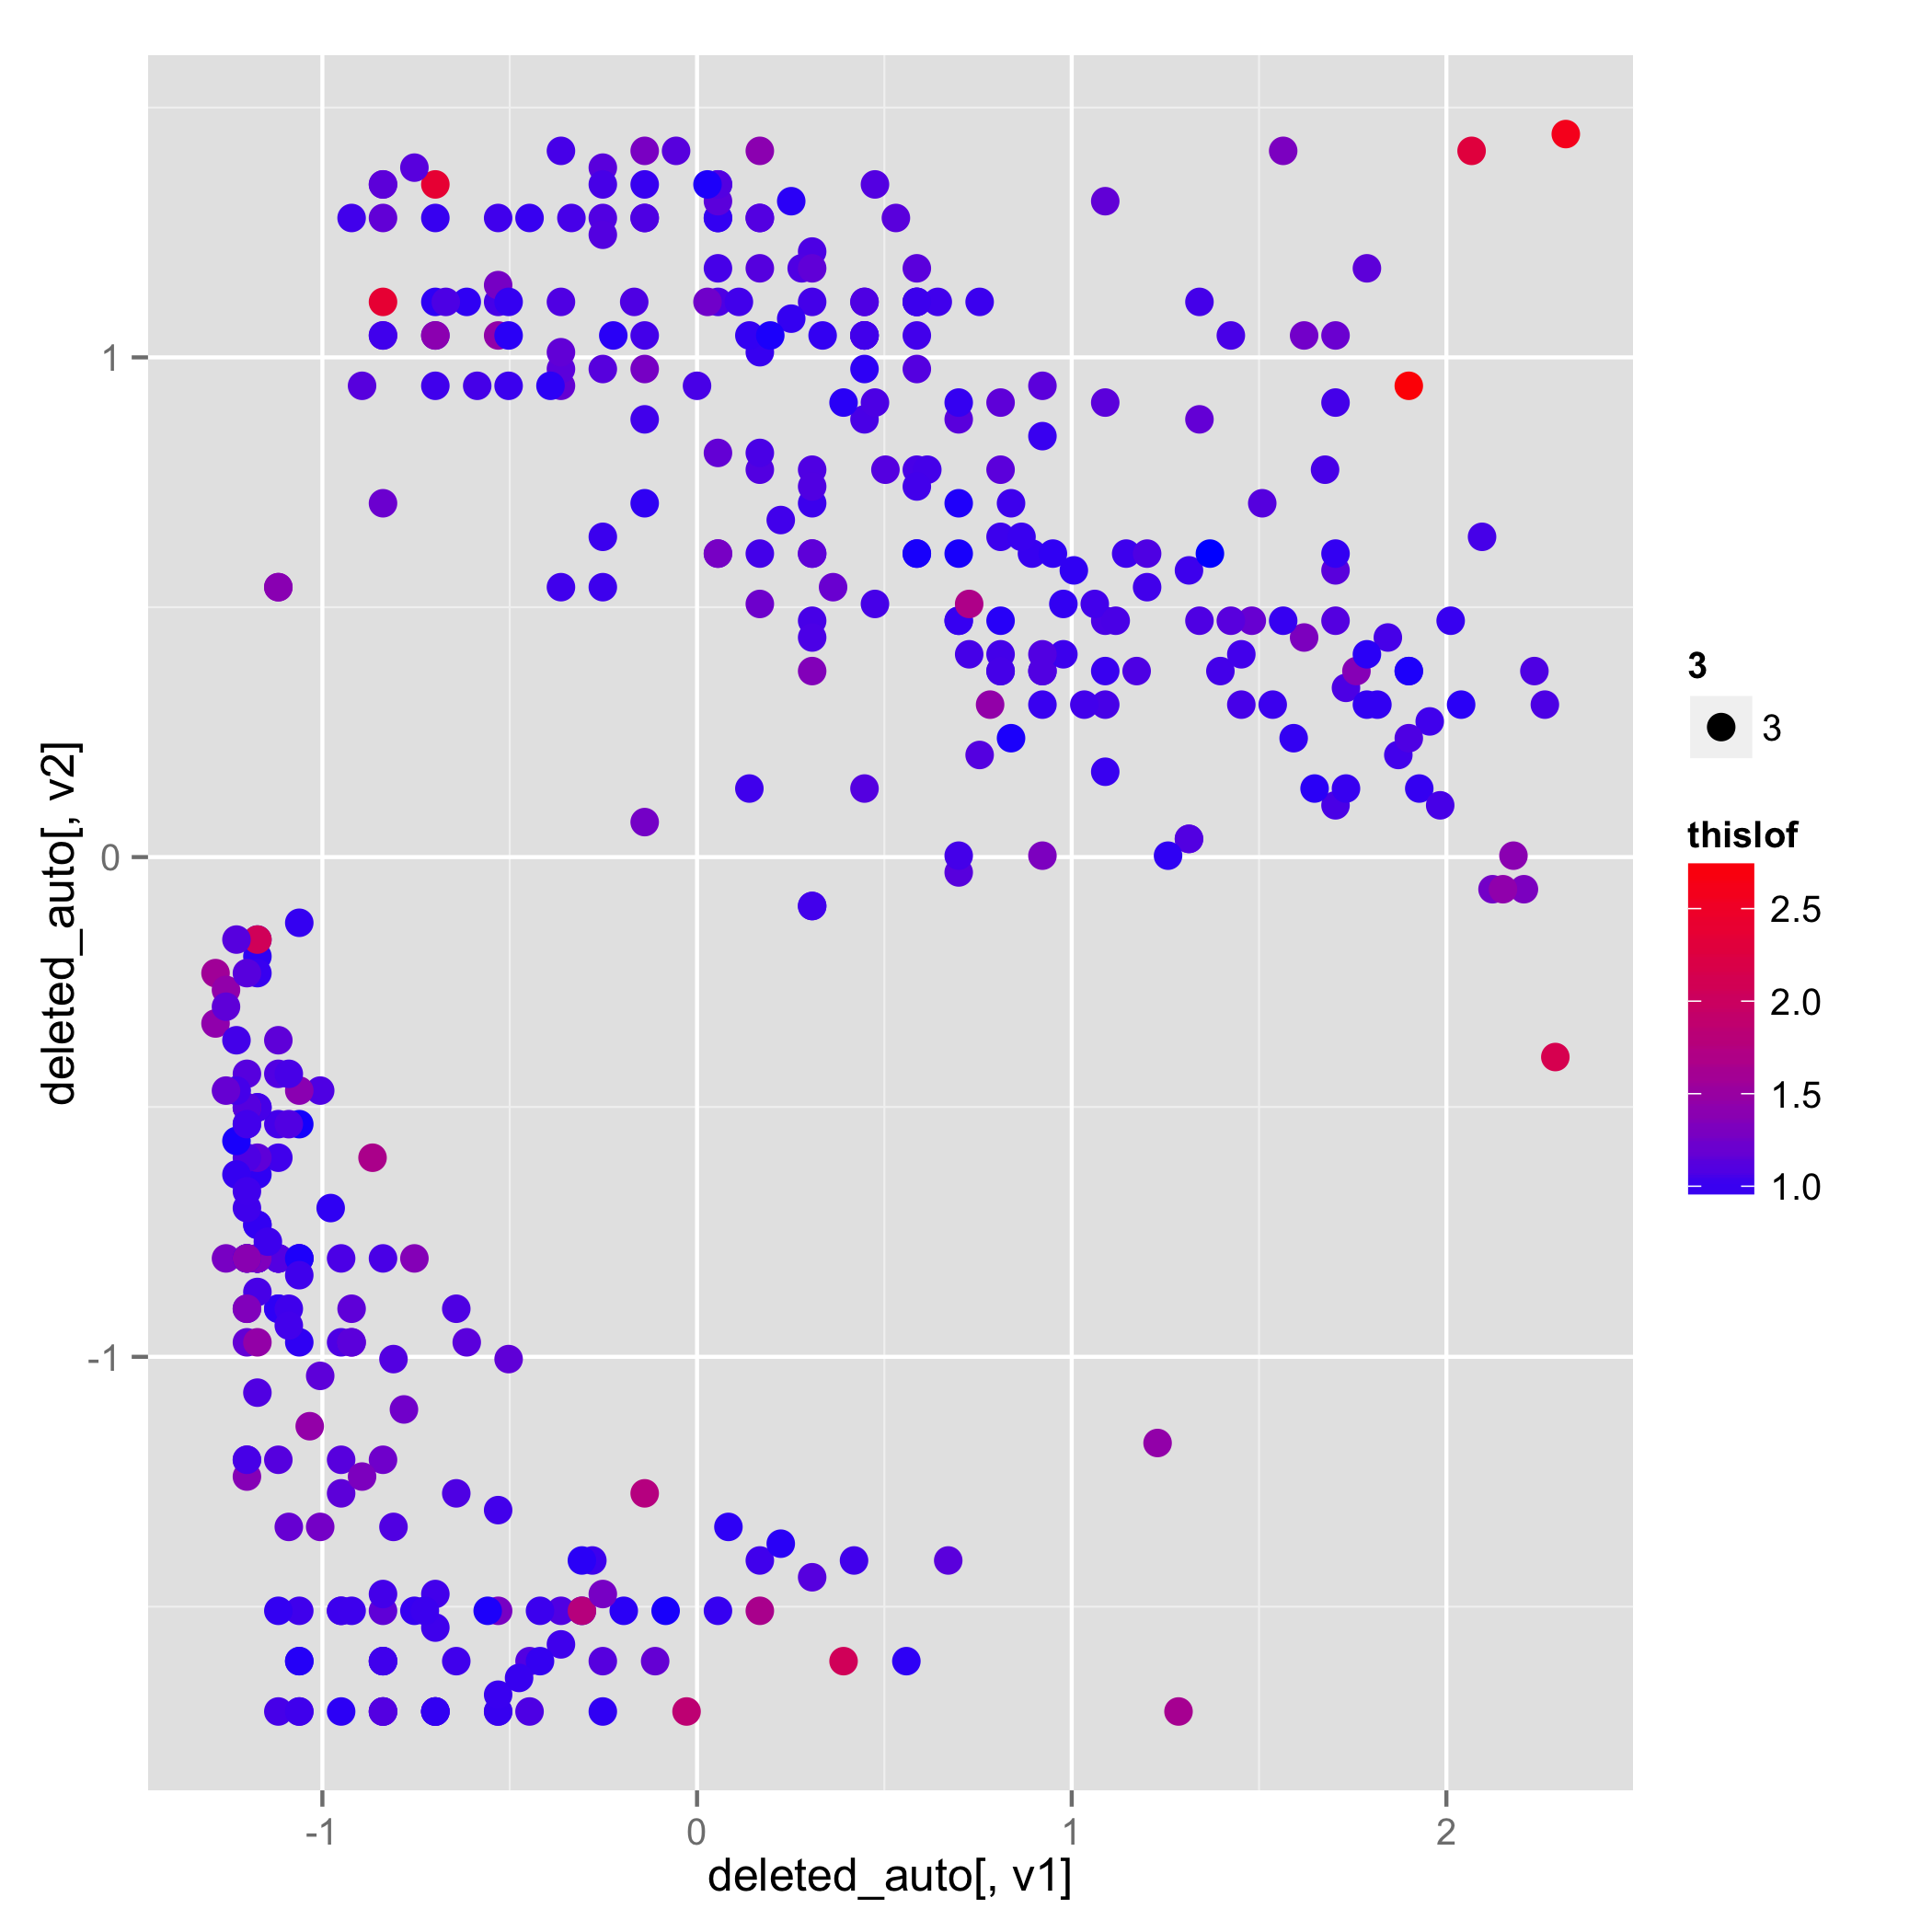
\includegraphics[scale=0.05]{using_lof1_4.png}
\par\end{centering}}
\quad{}
\subfloat[]{\begin{centering}
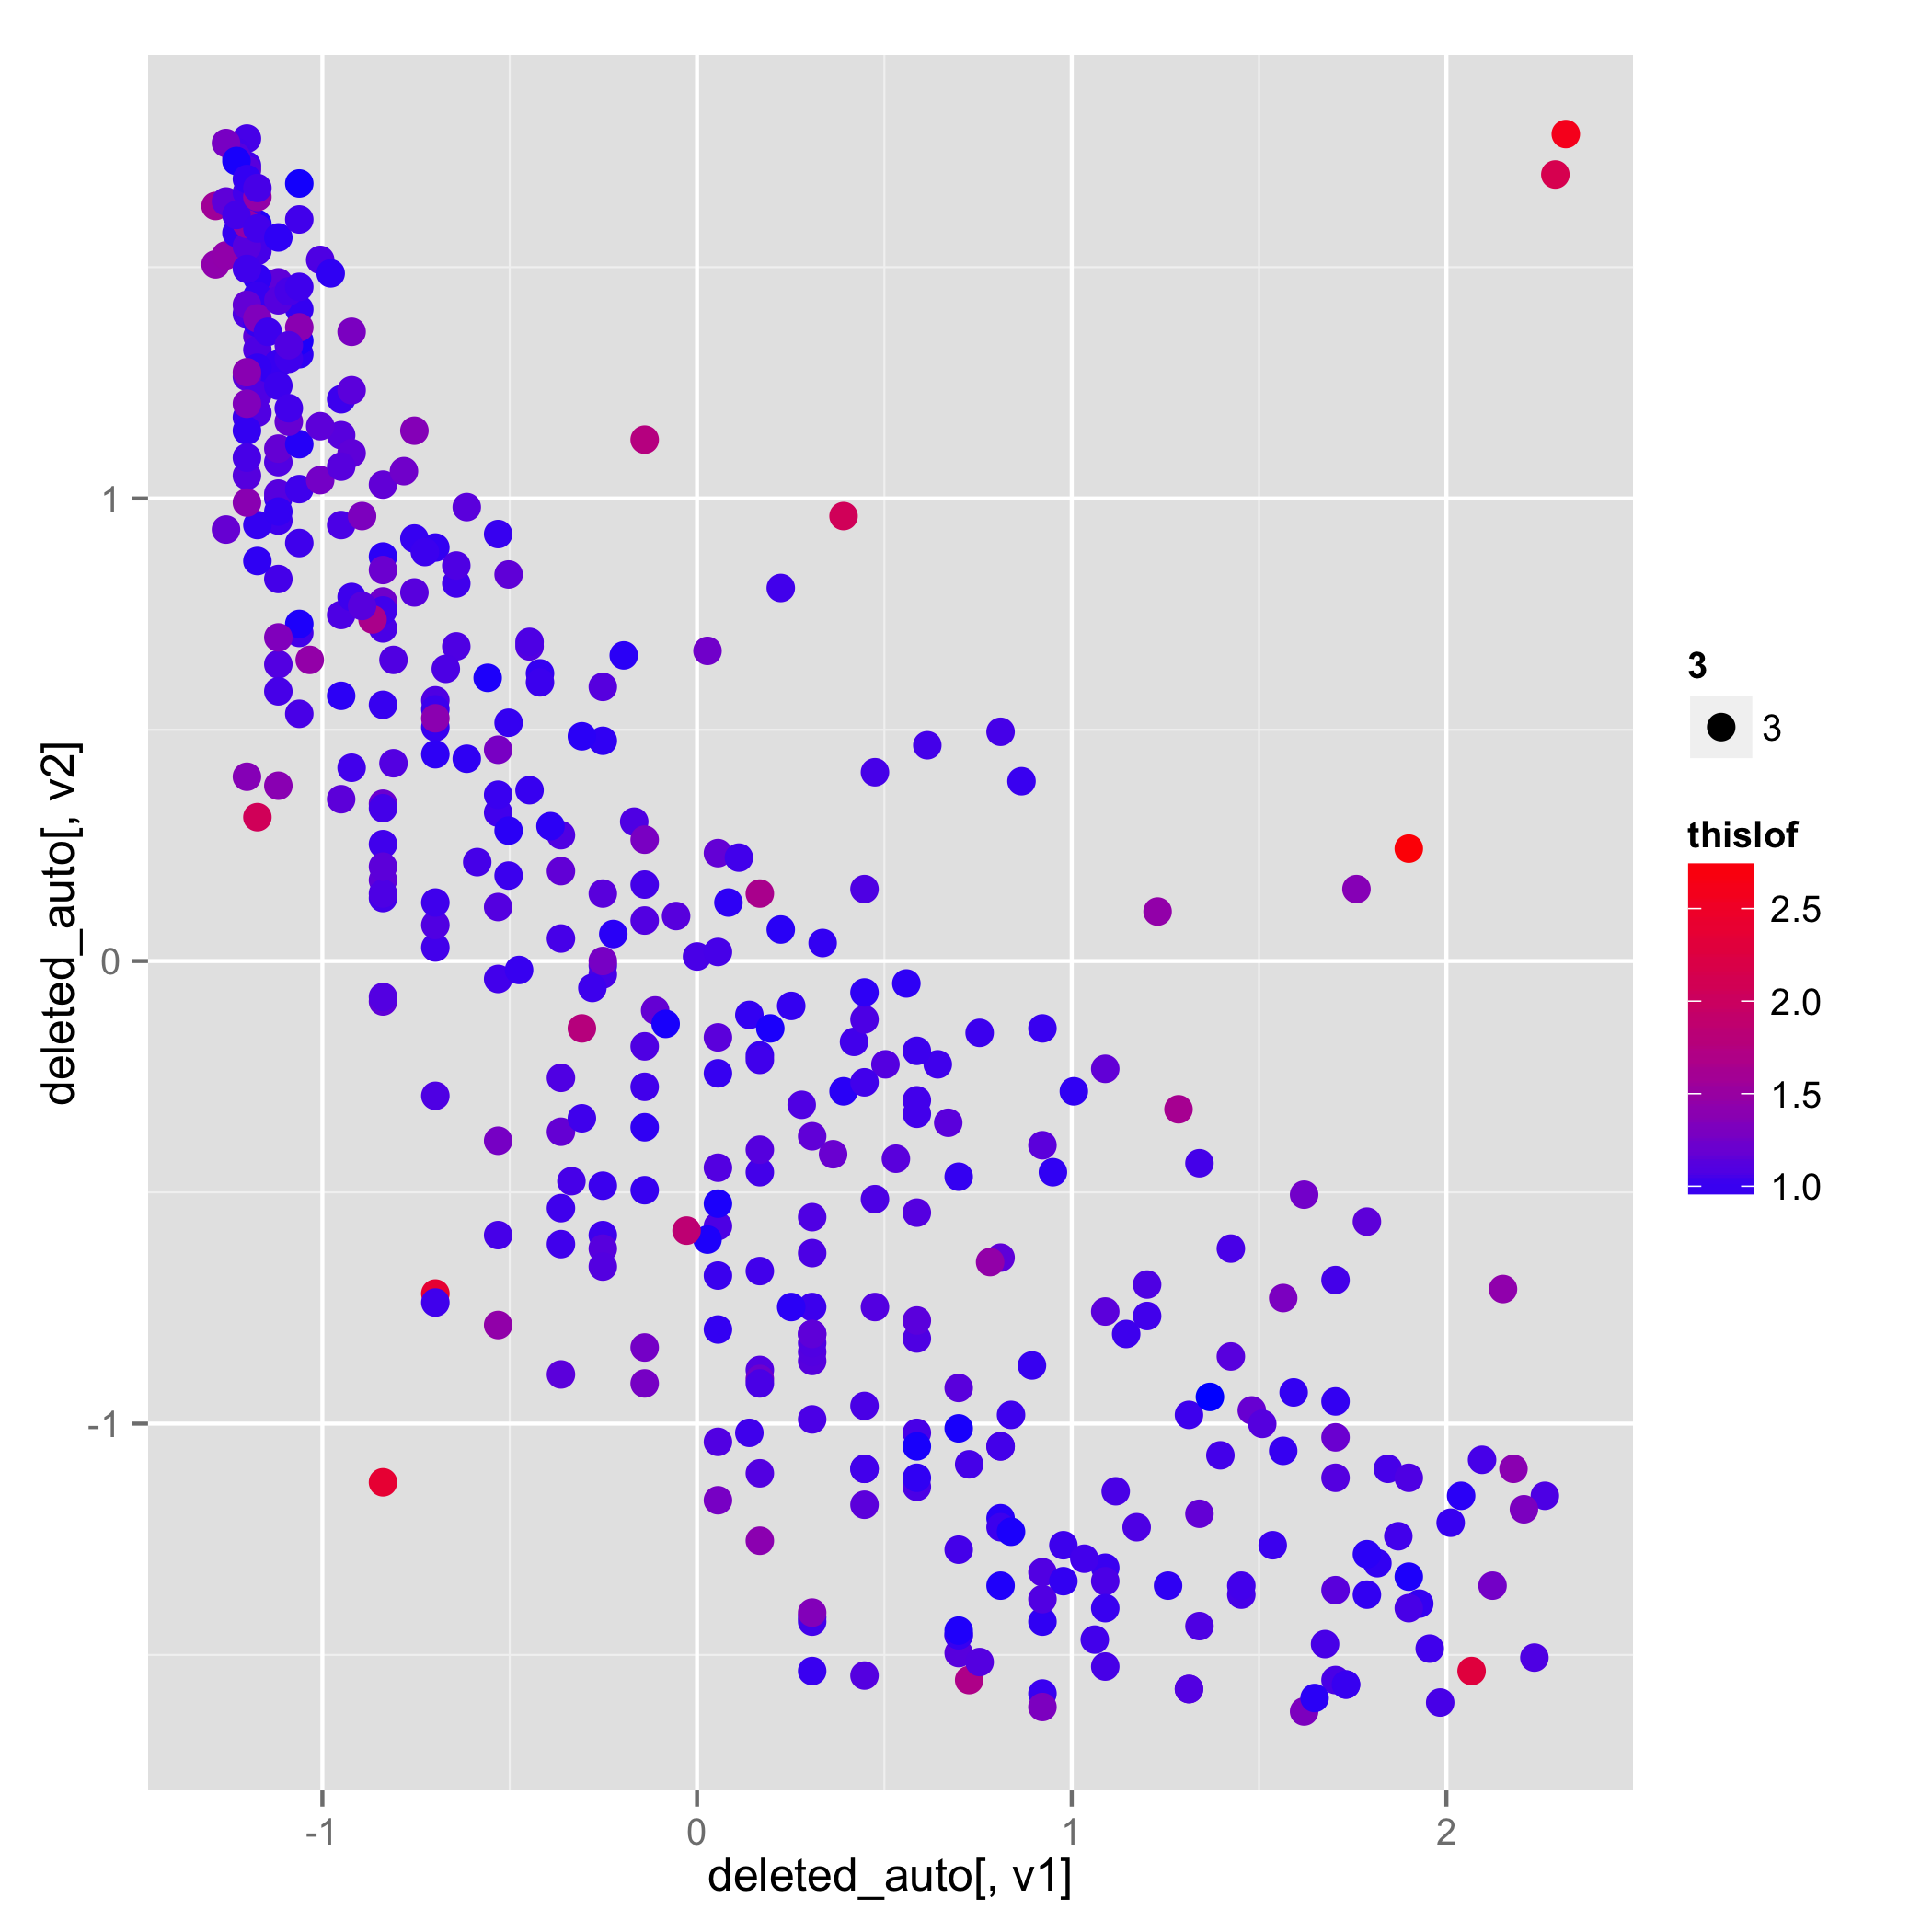
\includegraphics[scale=0.05]{using_lof1_5.png}
\par\end{centering}}
\quad{}
\subfloat[]{\begin{centering}
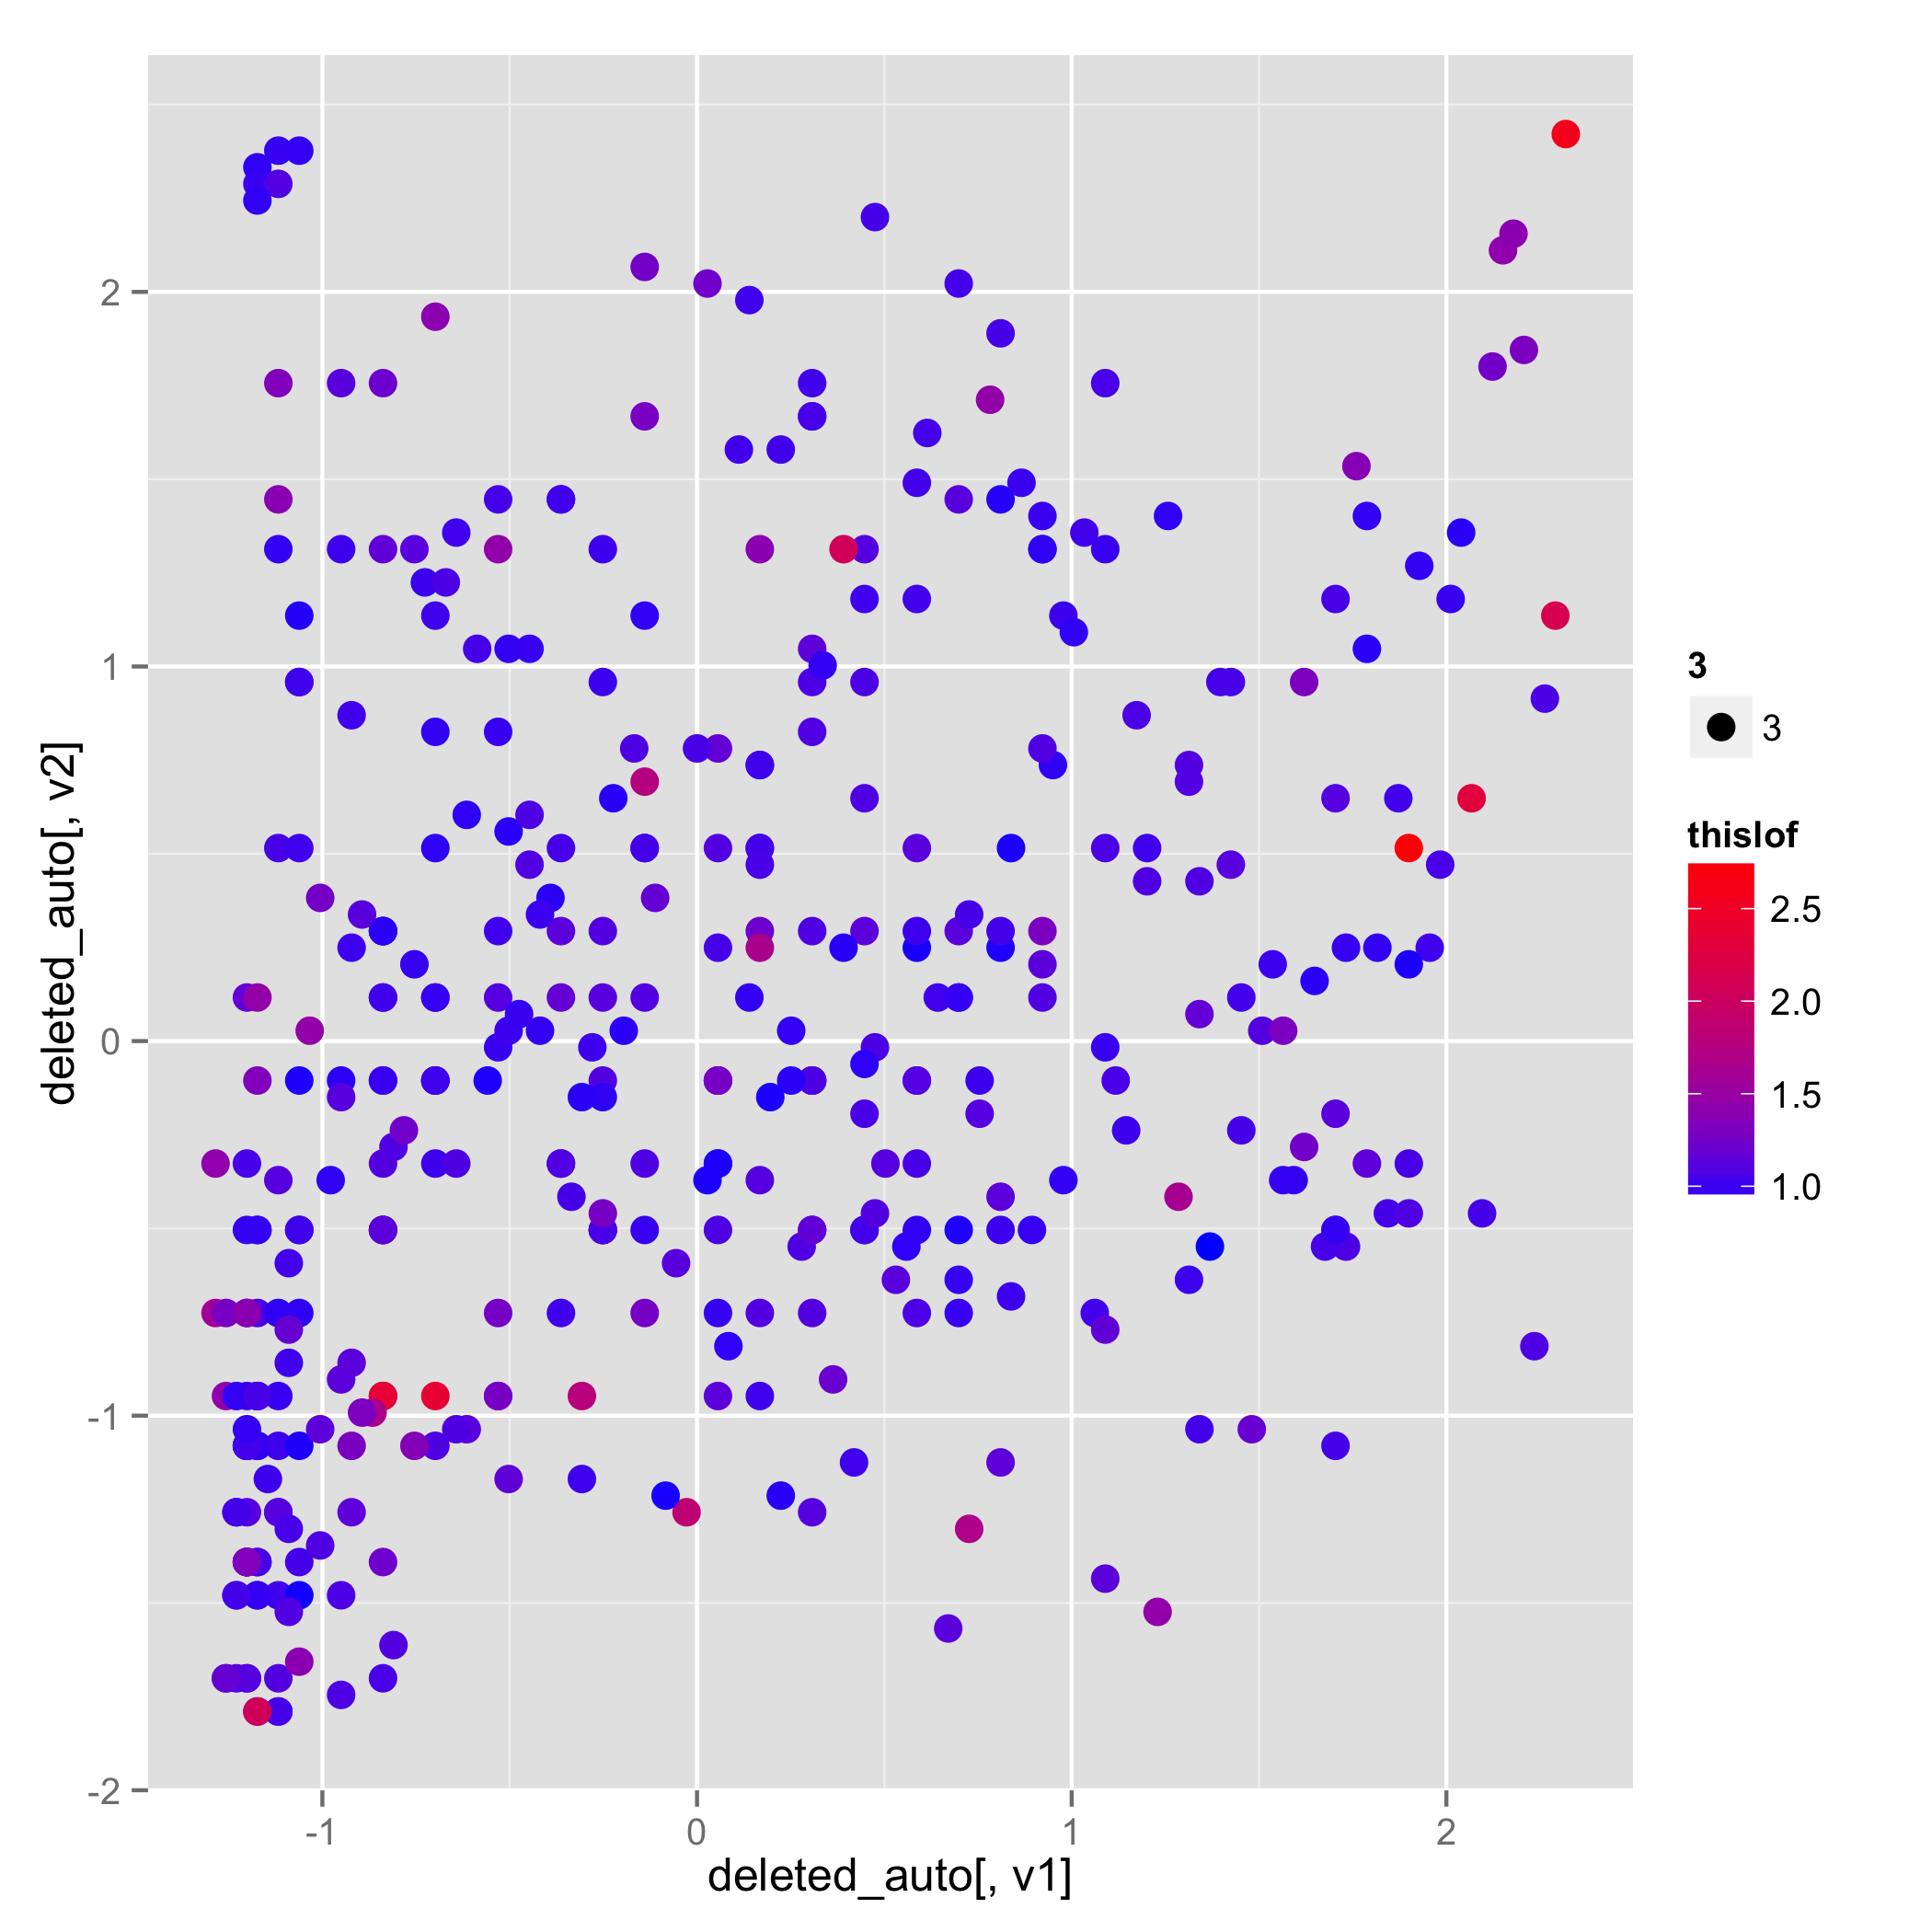
\includegraphics[scale=0.05]{using_lof1_6.png}
\par\end{centering}}
\quad{}
\subfloat[]{\begin{centering}
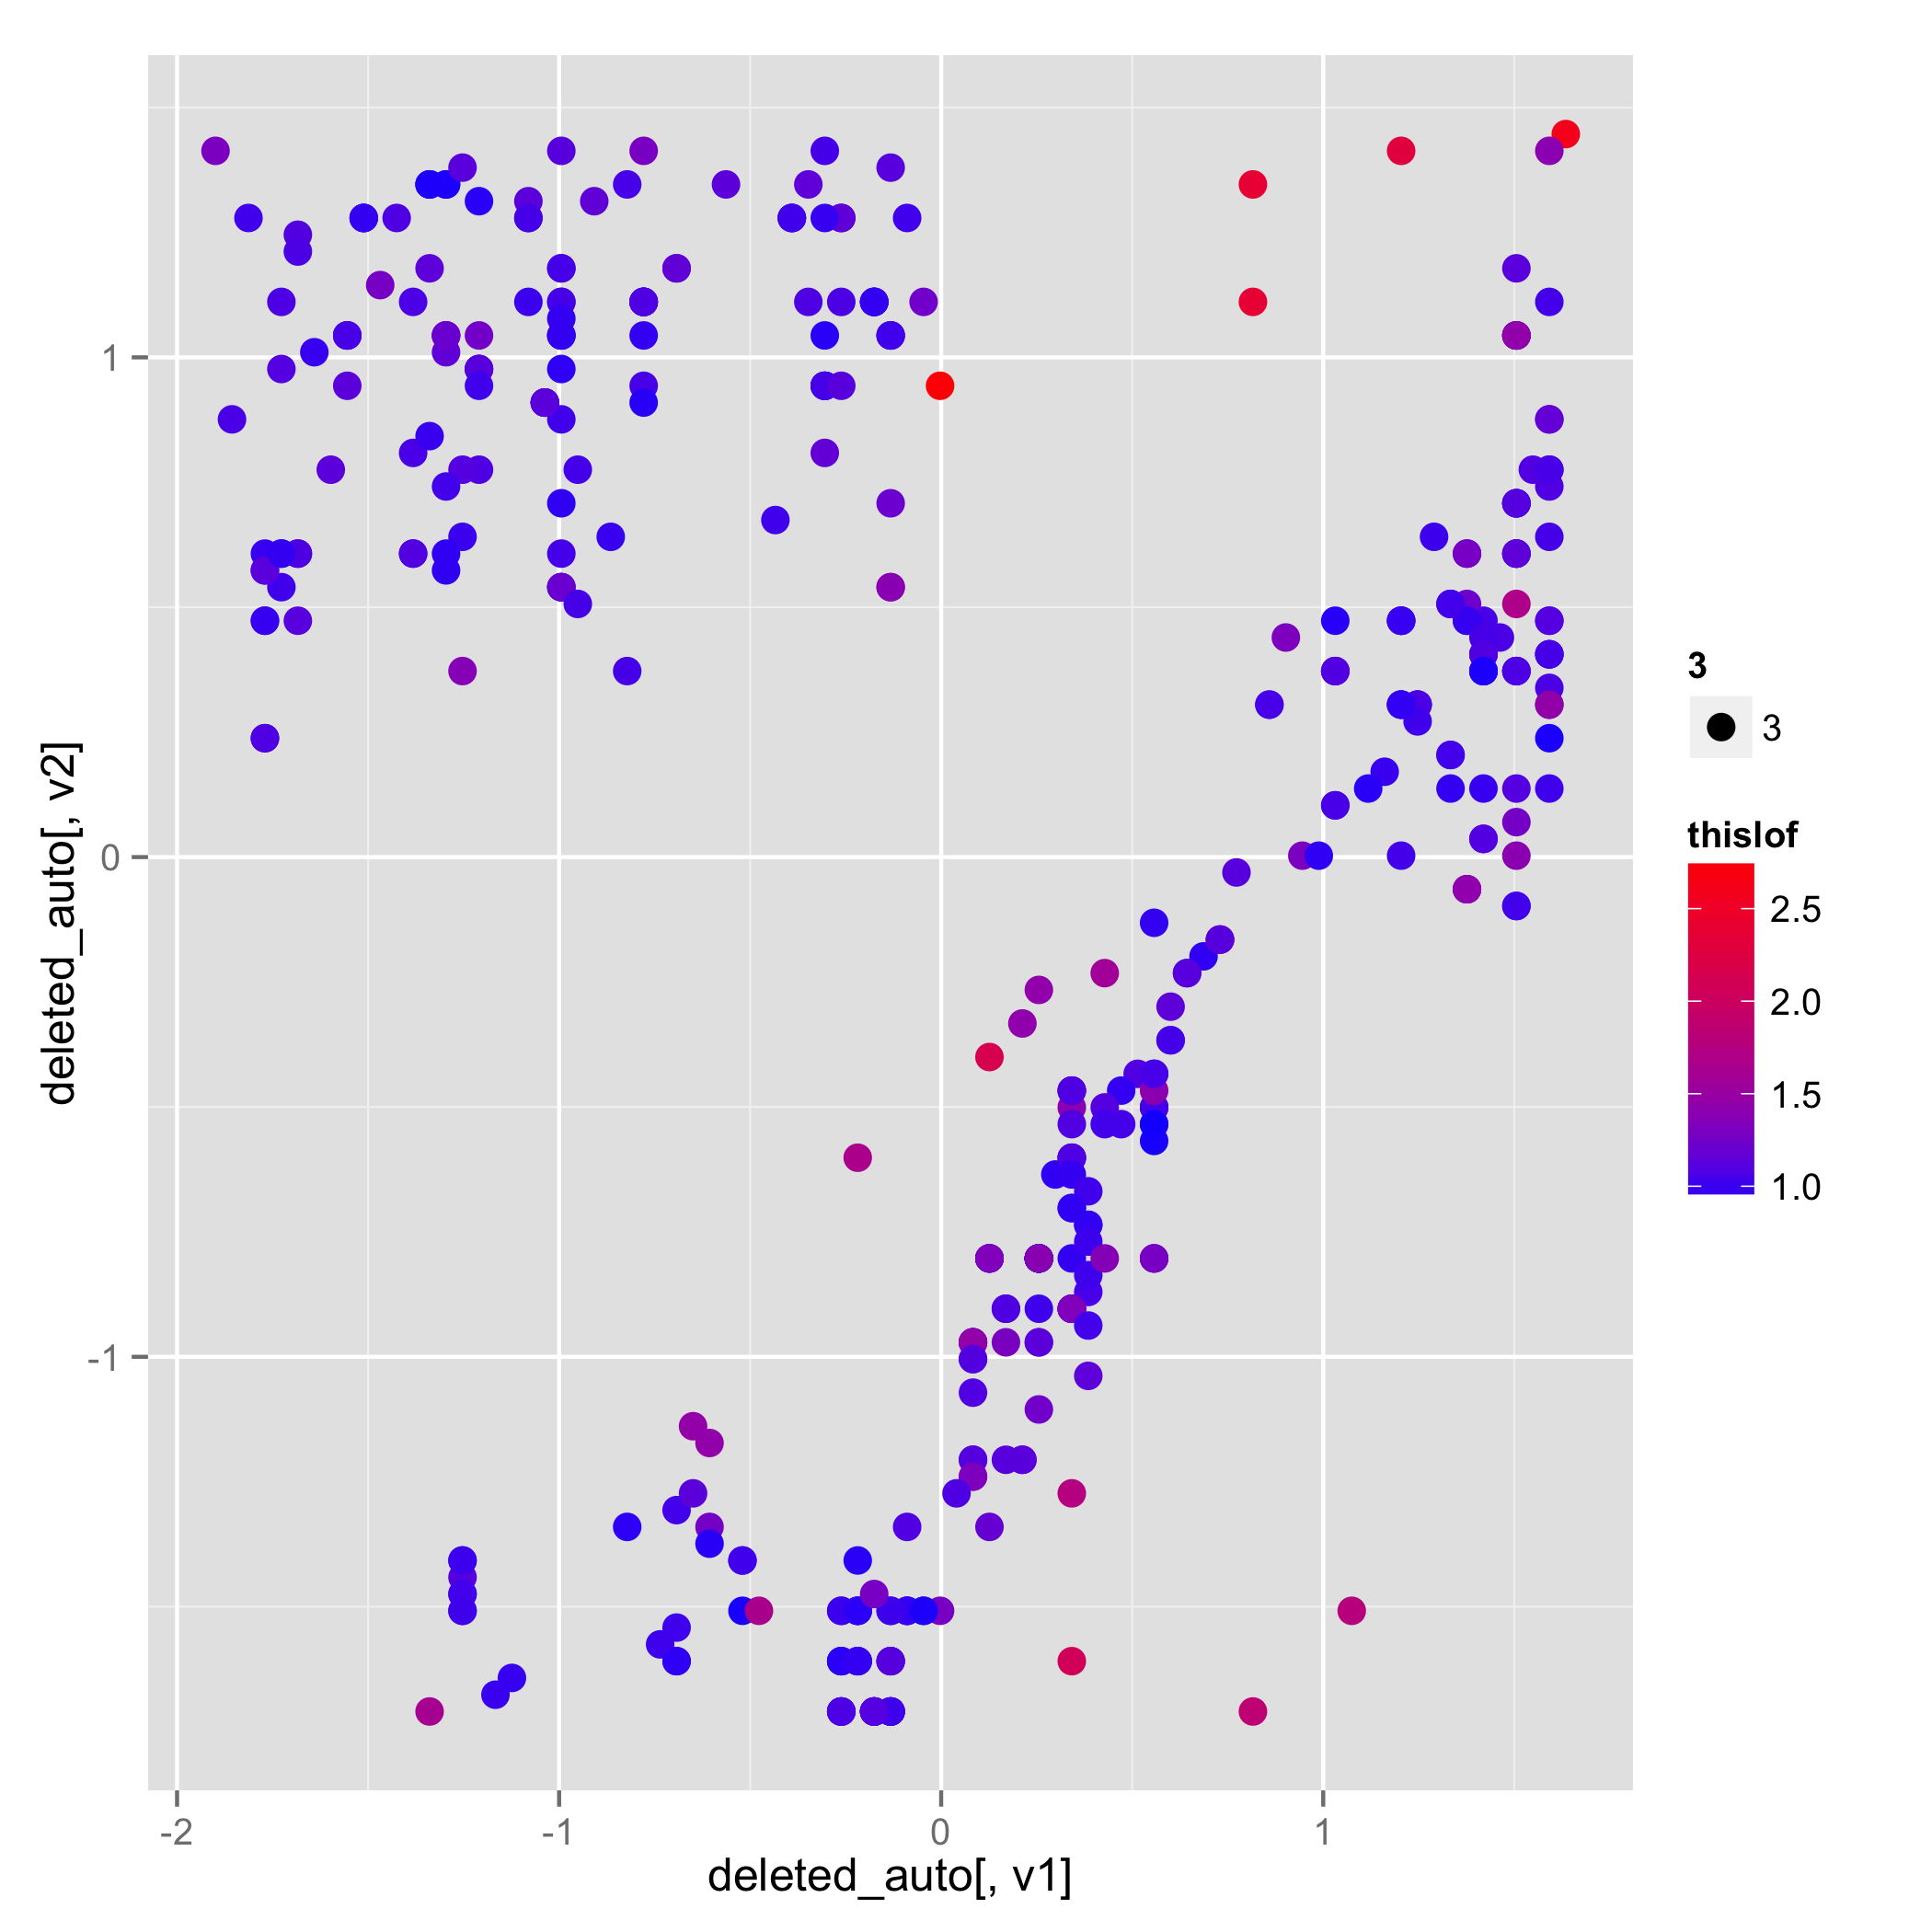
\includegraphics[scale=0.05]{using_lof3_4.png}
\par\end{centering}}
\quad{}
\subfloat[]{\begin{centering}
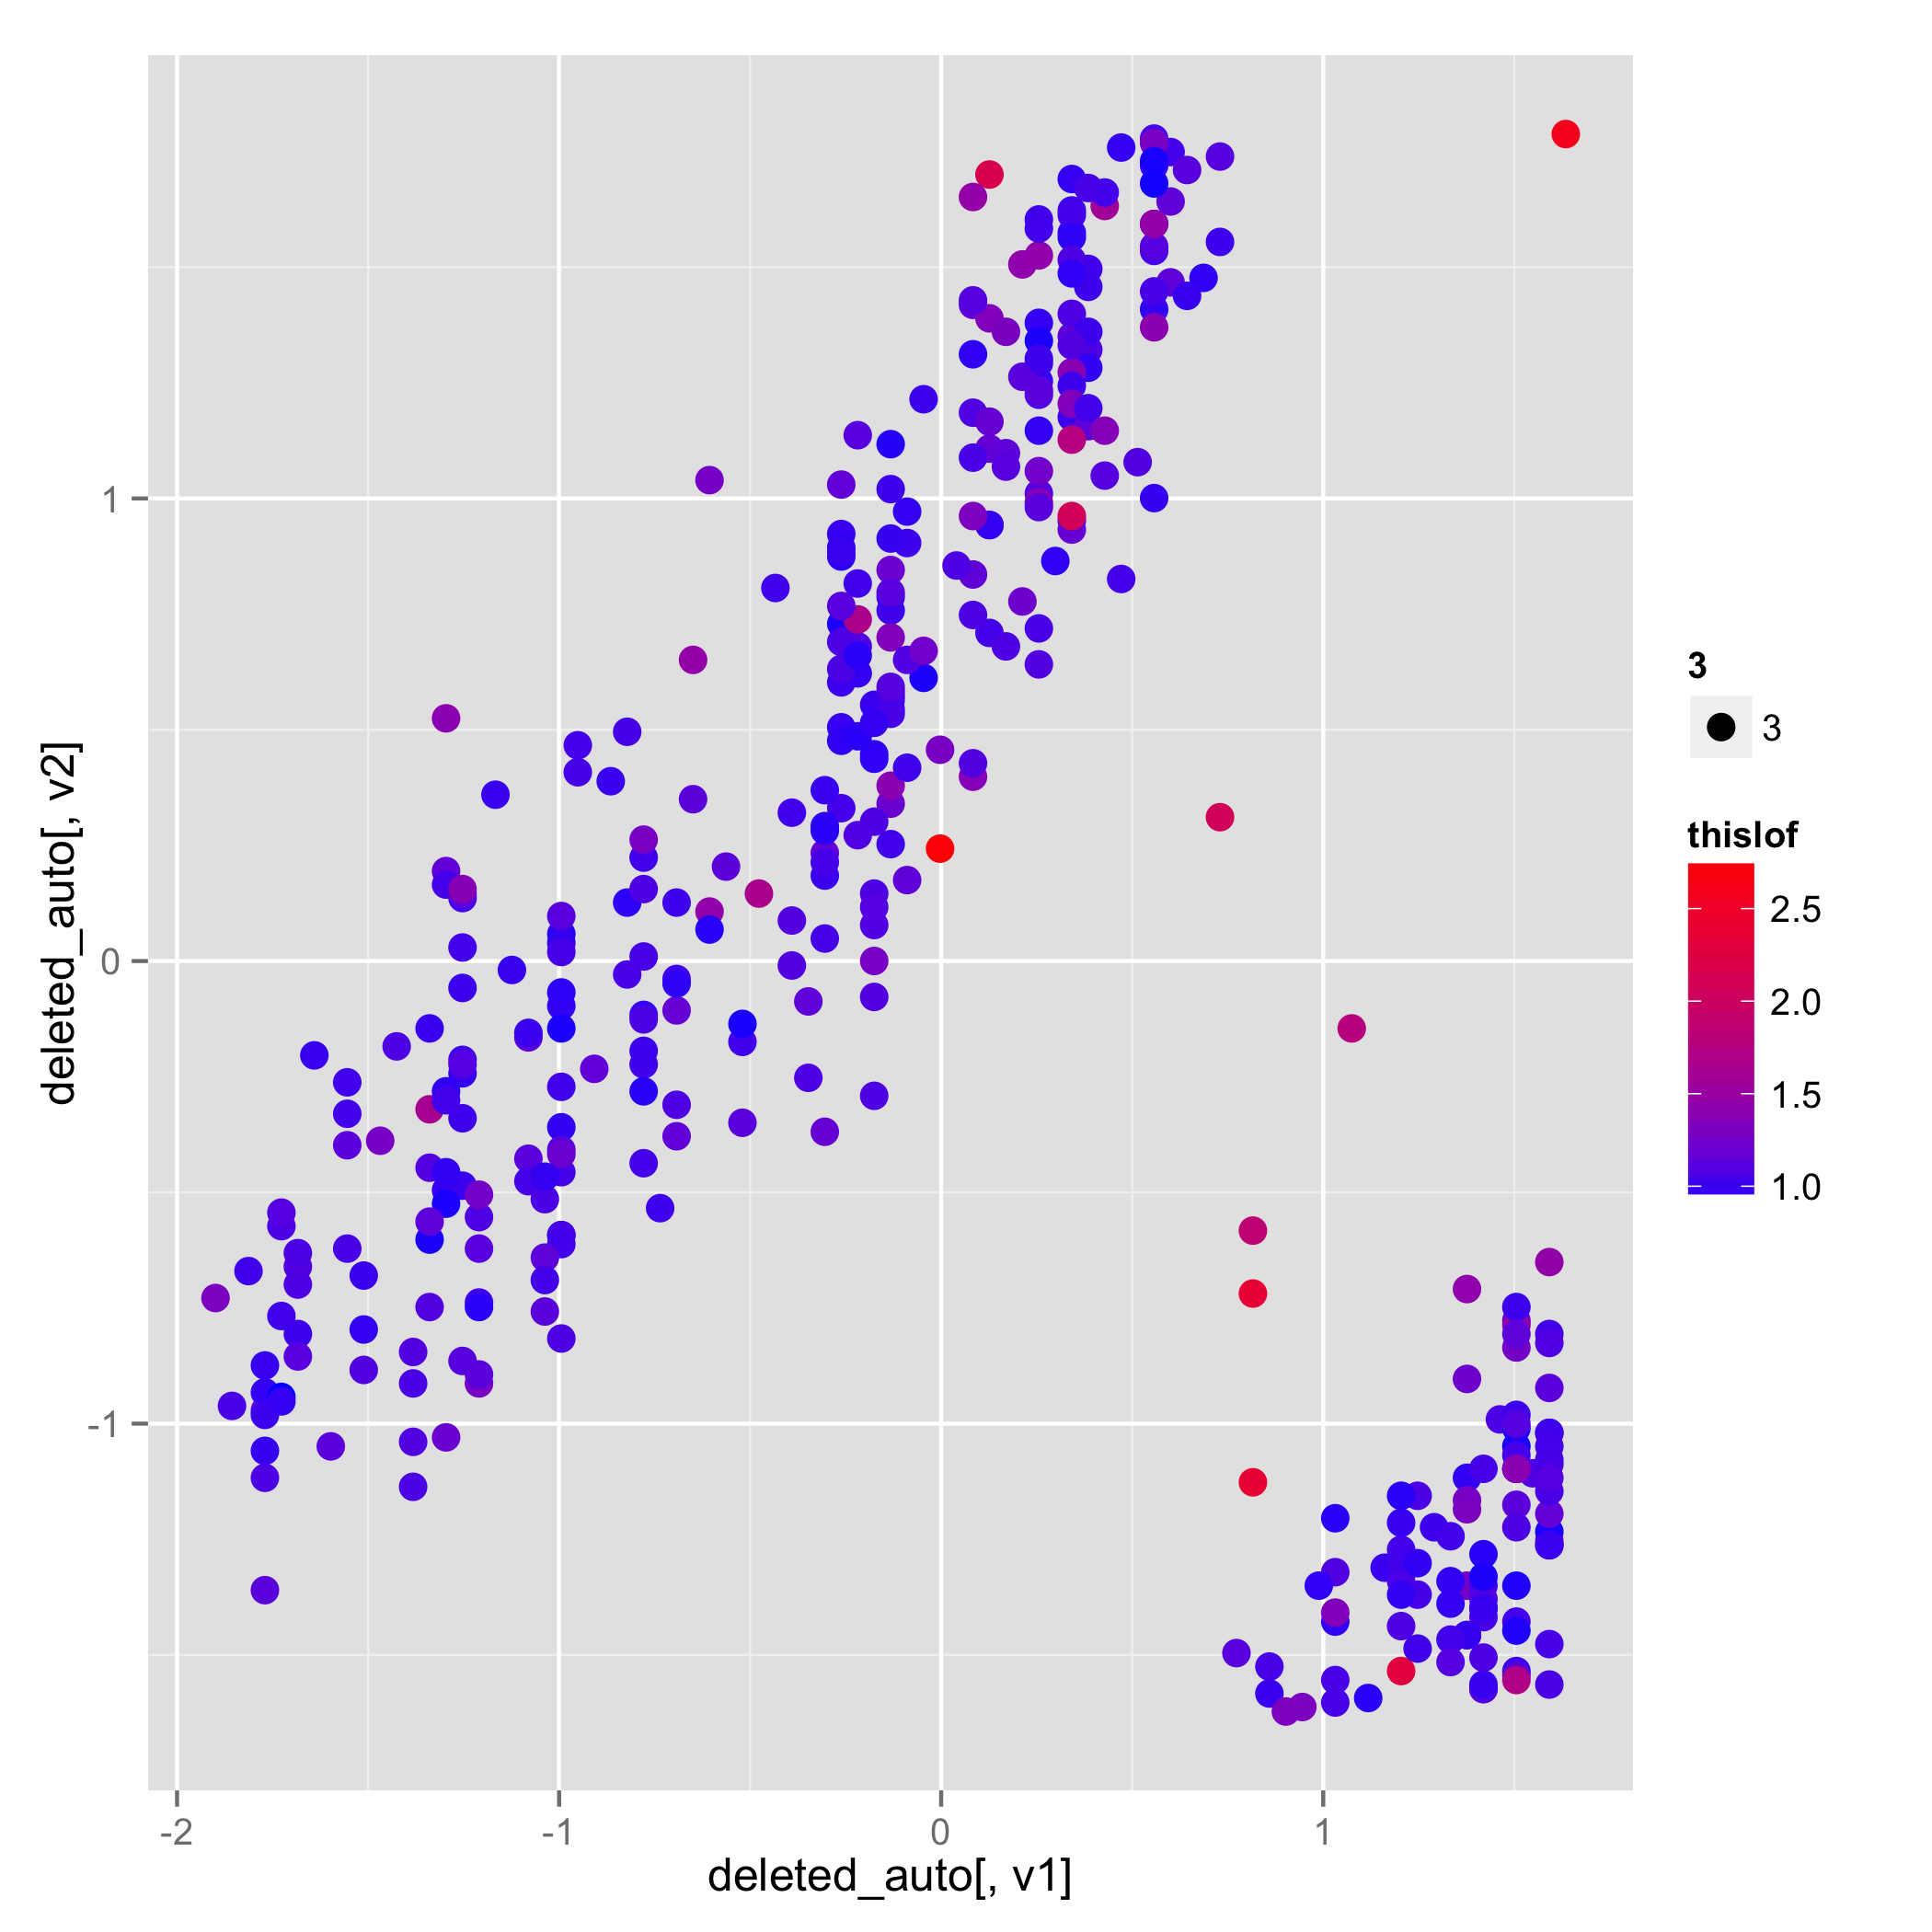
\includegraphics[scale=0.05]{using_lof3_5.png}
\par\end{centering}}
\quad{}
\subfloat[]{\begin{centering}
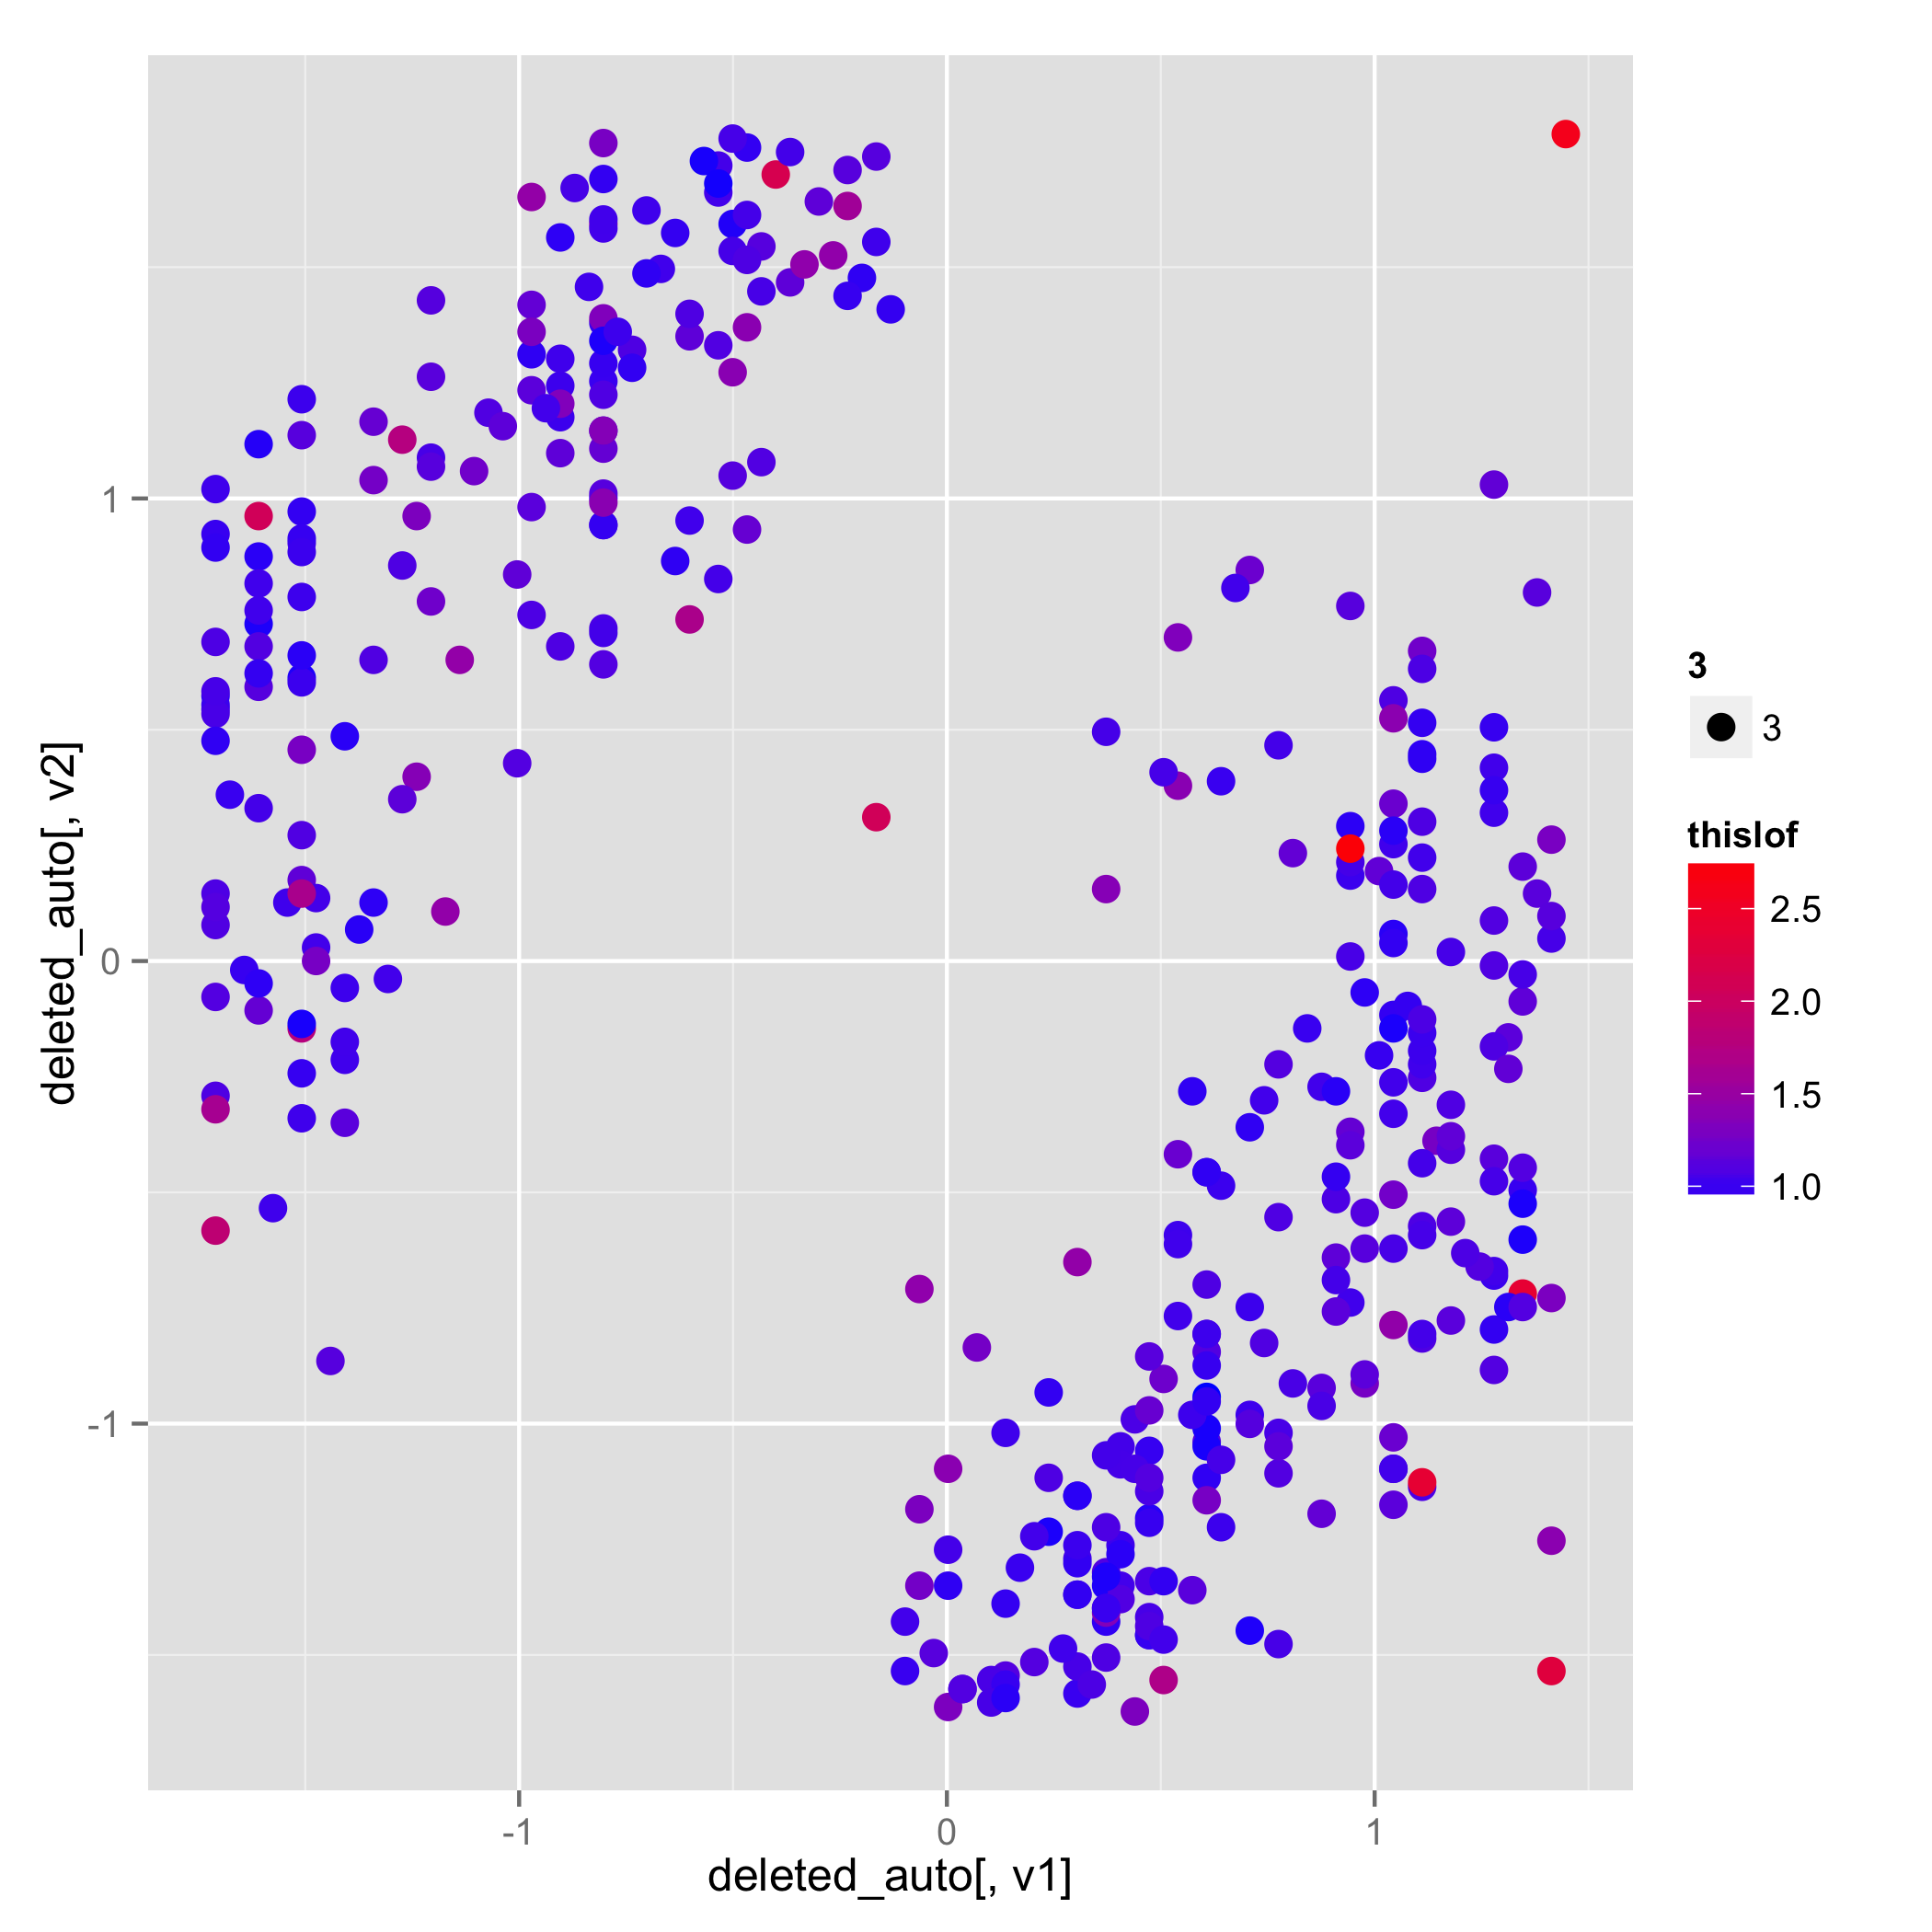
\includegraphics[scale=0.05]{using_lof4_5.png}
\par\end{centering}}
\quad{}
\subfloat[]{\begin{centering}
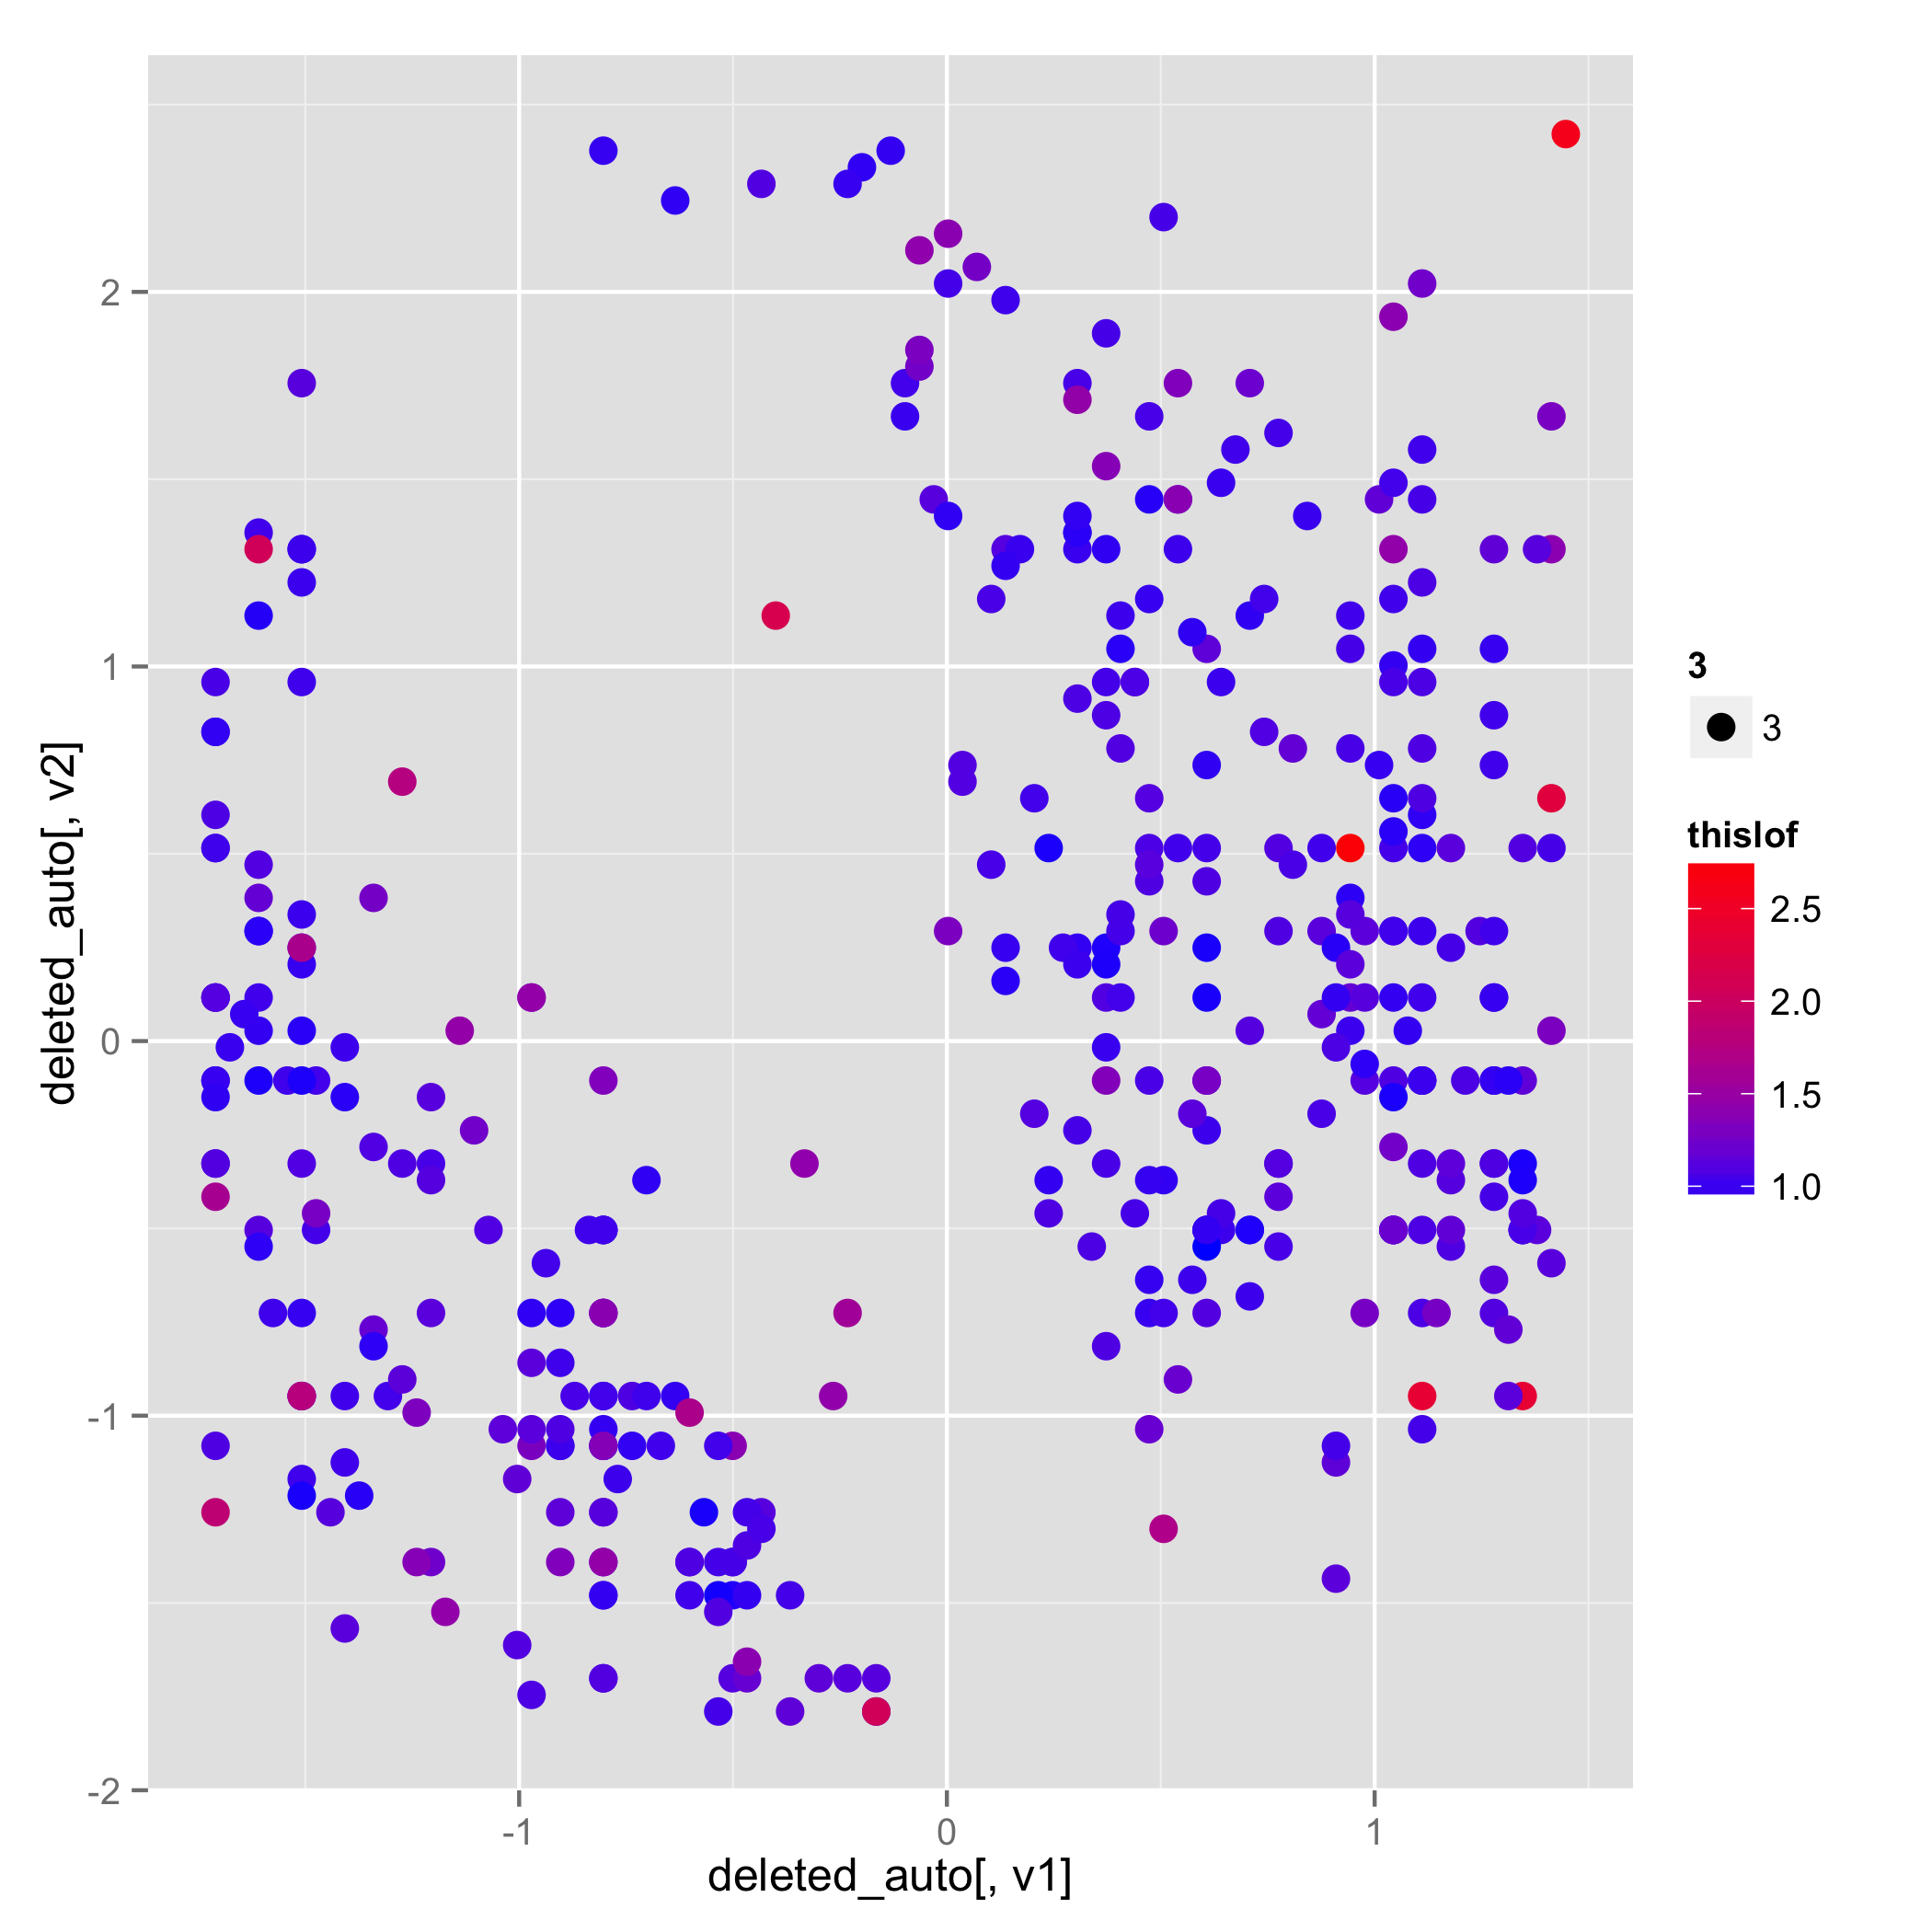
\includegraphics[scale=0.05]{using_lof4_6.png}
\par\end{centering}}
\quad{}
\subfloat[]{\begin{centering}
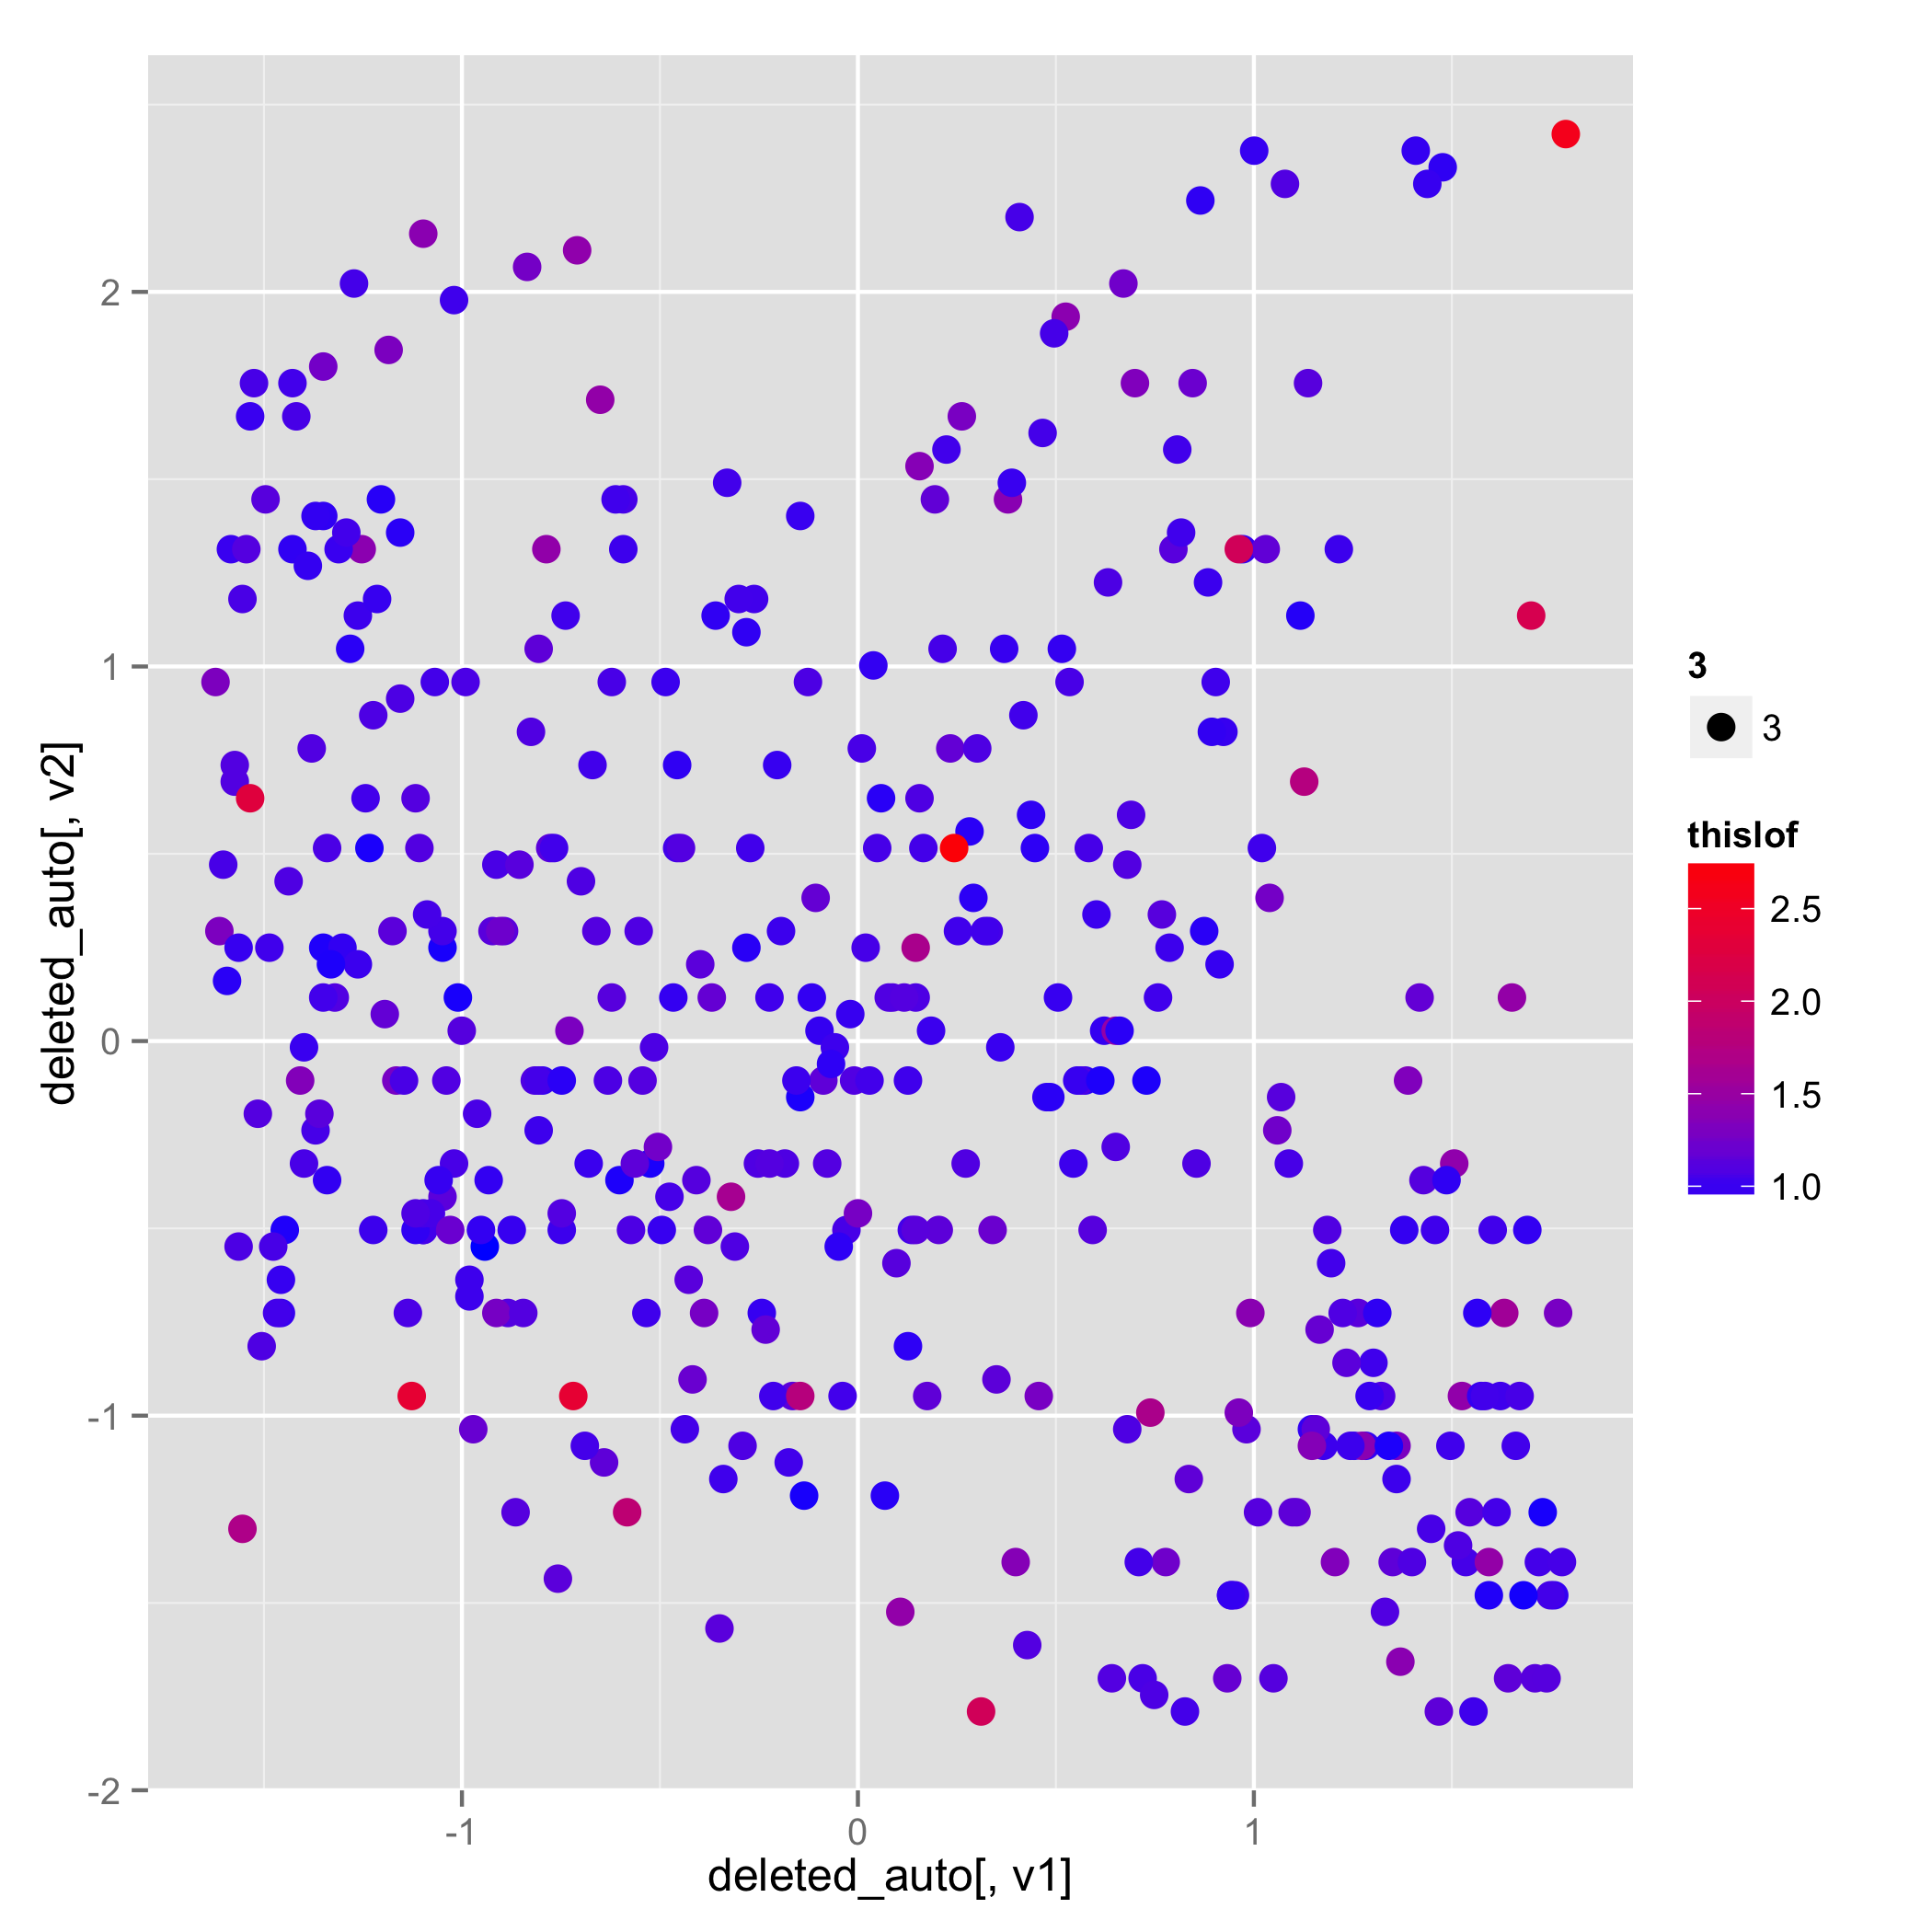
\includegraphics[scale=0.05]{using_lof5_6.png}
\par\end{centering}}
\end{center}
\end{figure}


The entries selected as outliers are shown below plotted in color, while the remaining entries are colored black. 

\begin{center}
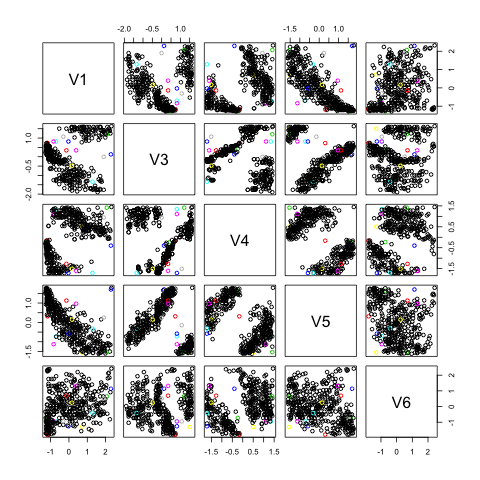
\includegraphics[scale=0.35]{all_plot}
\end{center}

\end{itemize}


The values categorized as outliers are shown below for each of the three methods with the different cutoff values discussed. 

\begin{center}
\begin{tabular}{| c | c | l |}
\hline
Metric & cutoff value & outliers\\ \hline
Distance & 1.25 & 1, 30,  73, 113, 211, 245, 329, 335, 336, 359, 366, 389 \\ \hline
& 1.5 & 1, 30, 113, 389 \\ \hline
Density & 5 & 41,  42,  43,  44,  45,  46,  65,  66,  67,  70,  71,  89,  94, 117, 158, 190, 192, 210\\ \hline
& 5.5 & 41,  43,  44,  45,  46,  65,  66,  67,  70,  89, 117, 190, 192, 210 \\ \hline
LOF & 1.5 & 1,  15,  27,  30,  73, 113, 205, 245, 265, 300, 332, 336, 359, 366, 388, 389 \\ \hline
\end{tabular}
\end{center}

The nodes chosen as outliers for Density were entirely different from those chosen by Distance metric or by local outlier factor 
metric. There were some in common between the latter two, although not all the same either. The variance in which entries were 
determined to be outliers between the three metrics makes it very difficult to tell whether any one of the values is indeed an outlier. 

There is some likelihood that the entries in rows 1, 113, and 389 are outliers as they occur in both of the rows associated with 
the distance metric as well as that associated with the local outlier factor metric. 

\end{enumerate}

\pagebreak
\lstinputlisting[language=R, basicstyle=\ttfamily\scriptsize]{hw21.R}

\end{document}
